\documentclass[10pt,letterpaper,oneside]{report}
\usepackage[T1]{fontenc}
\usepackage[utf8]{inputenc}
\usepackage{lmodern}
\usepackage[margin=0.78in,headheight=14pt]{geometry}
\usepackage{microtype}
\usepackage{amsmath,amssymb}
\usepackage{booktabs,tabularx,longtable,array}
\usepackage{enumitem}
\usepackage{xcolor,tikz}
\usetikzlibrary{arrows.meta,positioning,calc,fit,shapes.geometric}
\usepackage{listings}
\usepackage{caption}
\usepackage{fancyhdr}
\PassOptionsToPackage{obeyspaces}{url}
\usepackage{xurl}
\usepackage{hyperref}
\hypersetup{colorlinks=true,linkcolor=blue!45!black,urlcolor=blue!45!black,
 pdftitle={OpenRocket MIT: Application architecture and developer guide},
 pdfauthor={OpenRocket MIT development documentation},bookmarksnumbered=true}
\definecolor{ink}{HTML}{17334A}
\definecolor{accent}{HTML}{007B91}
\definecolor{pale}{HTML}{EEF5F9}
\definecolor{muted}{HTML}{526779}
\definecolor{warm}{HTML}{FFF6DD}
\pagestyle{fancy}
\fancyhf{}
\fancyhead[L]{\small\sffamily\color{muted}OPENROCKET MIT / ARCHITECTURE}
\fancyhead[R]{\small\sffamily\color{muted}Source edition 6.4}
\fancyfoot[L]{\small\sffamily Architecture and implementation contracts}
\fancyfoot[R]{\small\sffamily\thepage}
\renewcommand{\headrulewidth}{0.3pt}
\widowpenalty=10000
\clubpenalty=10000
\setlength{\parindent}{0pt}
\setlength{\parskip}{5pt}
\setlength{\emergencystretch}{2em}
\setlist{nosep,leftmargin=1.4em,topsep=4pt}
\renewcommand{\arraystretch}{1.18}
\captionsetup{font=small,labelfont={bf,color=ink},skip=8pt}
\newcolumntype{L}[1]{>{\raggedright\arraybackslash}p{#1}}
\newcolumntype{Y}{>{\raggedright\arraybackslash}X}
\AddToHook{env/tabularx/begin}{\small}
\AddToHook{env/longtable/begin}{\small}
\newcommand{\code}[1]{\nolinkurl{#1}}
\newcommand{\class}[1]{\nolinkurl{#1}}
\newcommand{\us}{\ensuremath{\,\mu\mathrm{s}}}
\newcommand{\ms}{\ensuremath{\,\mathrm{ms}}}
\newcommand{\api}[2]{\href{../improvements/javadoc/#1.html}{\texttt{#2}}}
\lstset{basicstyle=\ttfamily\small,breaklines=true,columns=fullflexible,
 keepspaces=true,frame=single,rulecolor=\color{accent!35},backgroundcolor=\color{pale},
 xleftmargin=6pt,xrightmargin=6pt,aboveskip=8pt,belowskip=8pt,showstringspaces=false}
\tikzset{
 box/.style={draw=ink!75,fill=pale,rounded corners=2pt,align=left,
 inner sep=6pt,font=\fontsize{8}{10}\selectfont,minimum height=0.85cm},
 group/.style={draw=accent!45,dashed,rounded corners=3pt,inner sep=8pt},
 use/.style={-{Latex[length=5pt]},draw=ink!80,line width=0.55pt},
 inherit/.style={-{Triangle[open,length=7pt,width=6pt]},draw=ink!80,line width=0.6pt},
 own/.style={{Diamond[fill=ink,length=6pt,width=4pt]}-,draw=ink!80,line width=0.6pt},
 flowlabel/.style={font=\fontsize{7.5}{9}\selectfont,fill=white,inner sep=2pt,align=center},
 note/.style={draw=accent!30,fill=warm,rounded corners=2pt,align=left,inner sep=6pt,
 font=\fontsize{8}{10}\selectfont},
 lifeline/.style={draw=muted!65,densely dashed},
 participant/.style={box,align=center,minimum height=1cm,font=\fontsize{8}{10}\selectfont}
}
\newcommand{\uml}[5]{\node[box,text width=#5] (#1) at (#2)
 {\centering\bfseries\ttfamily #3\par\vspace{2pt}\hrule\vspace{3pt}
 \raggedright\normalfont\ttfamily #4};}
\newcommand{\simple}[4]{\node[box,text width=#4,align=center] (#1) at (#2)
 {\bfseries\ttfamily #3};}
\newcommand{\diagram}[3]{\begin{figure}[htbp]\centering
\resizebox{\linewidth}{!}{#3}\caption{#2}\label{#1}\end{figure}}

\usepackage{titlesec}
\usepackage{needspace}
\titleformat{\chapter}[display]{\sffamily\bfseries\color{ink}\raggedright\hyphenpenalty=10000\exhyphenpenalty=10000}{\large CHAPTER \thechapter}{8pt}{\Huge}
\titlespacing*{\chapter}{0pt}{0pt}{18pt}
\titleformat{\section}{\Large\sffamily\bfseries\color{ink}}{\thesection}{0.7em}{}
\titleformat{\subsection}{\large\sffamily\bfseries\color{ink}}{\thesubsection}{0.7em}{}
\fancypagestyle{plain}{\fancyhf{}\fancyfoot[L]{\small\sffamily Architecture and implementation contracts}\fancyfoot[R]{\small\sffamily\thepage}\renewcommand{\headrulewidth}{0pt}}
\newcommand{\source}[2]{\href{https://github.com/MDNich/ActiveControl_MIT_RktTeam/blob/7f0b67ee1c755ec89f154b0f0d2f4e23c843aa87/clone/openrocket-release-24.12.RC.01/#1}{\nolinkurl{#2}}}
\newcommand{\reposource}[2]{\href{https://github.com/MDNich/ActiveControl_MIT_RktTeam/blob/7f0b67ee1c755ec89f154b0f0d2f4e23c843aa87/#1}{\nolinkurl{#2}}}
\newcommand{\sourceline}[1]{\par\smallskip{\small\color{muted}\textbf{Source entry points.} #1}\par}
\newenvironment{contract}{\begin{quote}\small\color{ink}\textbf{Implementation boundary.} }{\end{quote}}
\setcounter{secnumdepth}{2}
\setcounter{tocdepth}{1}

\begin{document}
\hypersetup{pageanchor=false}
\begin{titlepage}
\color{ink}
{\sffamily\bfseries\Large OPENROCKET MIT\par}
\vspace{1.2cm}
{\sffamily\bfseries\Huge Application architecture\par}
\vspace{0.2cm}
{\sffamily\bfseries\Huge and developer guide\par}
\vspace{0.7cm}
{\Large From the component tree to flight dynamics, desktop workflows, and onboard control\par}
\vspace{0.8cm}
{\large Source edition 6.4\quad /\quad 27 October 2026\par}
\vspace{0.6cm}\hrule height 1pt\vspace{0.5cm}
This guide explains how the MIT fork of OpenRocket is organized, how its major objects and services interact, and where to change or investigate each behavior. It follows a design through editing, configuration, numerical simulation, recovery, control, persistence, and visualization.

The flight-computer architecture report is incorporated as a complete chapter. Surrounding chapters explain the larger application that hosts it, including inherited OpenRocket capabilities and MIT-specific changes.
\vspace{0.5cm}
\begin{tabularx}{\linewidth}{@{}>{\bfseries}L{3.1cm}Y@{}}\toprule
Source snapshot & \code{7f0b67ee1c755ec89f154b0f0d2f4e23c843aa87}\\
Upstream basis & OpenRocket \code{release-24.12.RC.01}\\
Published baseline & MIT v6.4, source \code{9f71a941}, published 13 October 2026\\
Implementation & Java 17; Gradle root application, \code{core}, and \code{swing}\\
Reading level & Functional reference, physical models, architecture, execution contracts, and source navigation\\\bottomrule
\end{tabularx}
\vfill
{\small\color{muted}This is documentation of the inspected implementation, not a new numerical validation or hardware qualification. Current source and released packages differ despite sharing the 6.4 version label. Source links are pinned to the inspected commit.}\par
\end{titlepage}
\pagenumbering{roman}
\hypersetup{pageanchor=true}
{\small\setlength{\parskip}{0pt}\tableofcontents}
\clearpage
{\small\setlength{\parskip}{0pt}\listoffigures}
\clearpage\pagenumbering{arabic}
\chapter{How the application fits together}\label{ch:map}
OpenRocket is built around a persistent rocket model. The editor changes it; physical calculators derive its properties; an event-driven simulation advances it through flight; result objects preserve the output for analysis. The MIT edition adds active-control hardware, a virtual flight computer, repeated-run analysis, and corresponding desktop workflows.

Distinguish \emph{design}, \emph{configuration}, \emph{execution}, and \emph{observation}. A fin's span belongs to the design; its installed motor to a configuration; current angular velocity to a running simulation; and recorded roll rate to a result. These owners and lifetimes prevent stale results, unintended edits, and incorrect state reuse.

\section{The application-wide dependency map}
\diagram{fig:application-map}{Major application layers. Arrows indicate use or data flow; the return path through results does not modify the design automatically.}{%
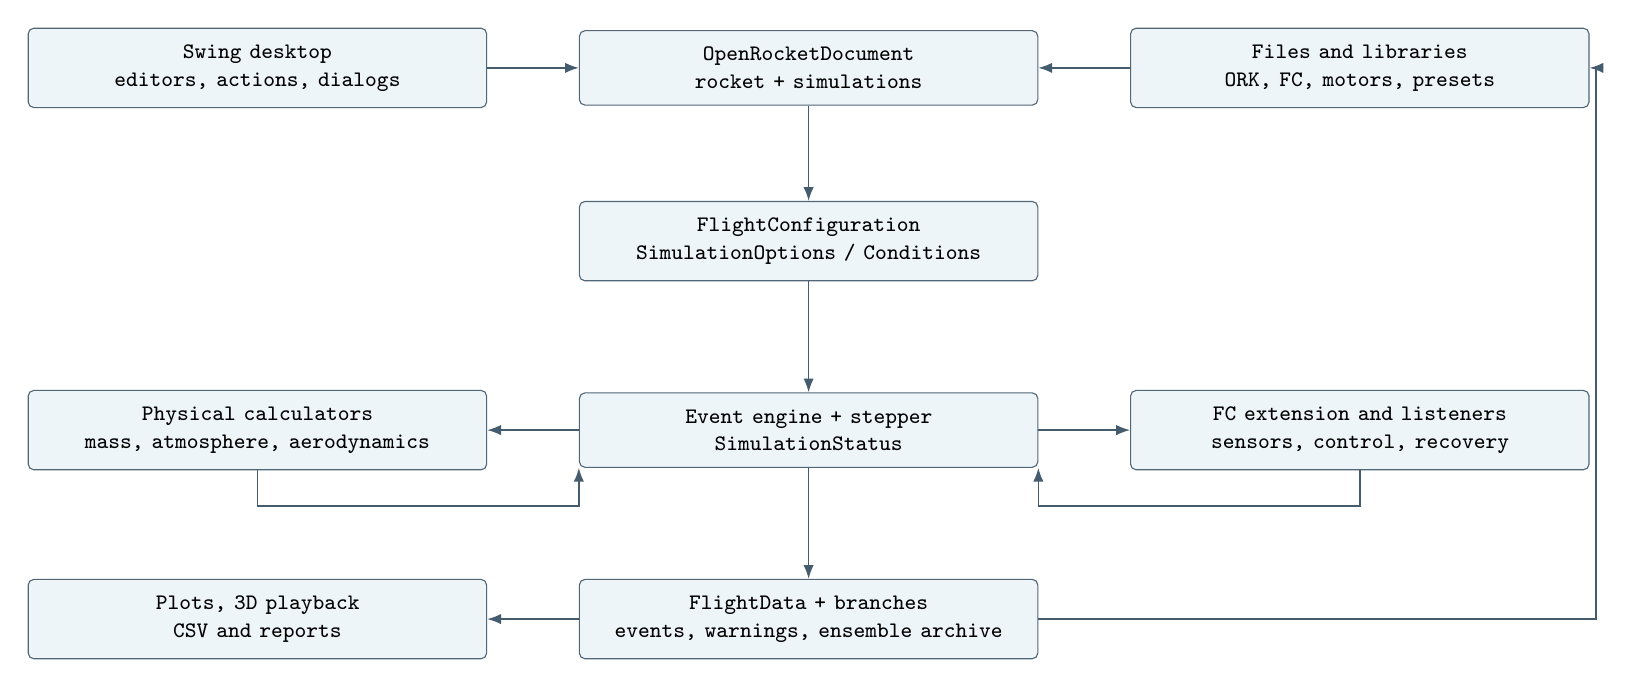
\begin{tikzpicture}
\simple{ui}{0,0}{Swing desktop\\editors, actions, dialogs}{5.4cm}
\simple{doc}{7,0}{OpenRocketDocument\\rocket + simulations}{5.4cm}
\simple{files}{14,0}{Files and libraries\\ORK, FC, motors, presets}{5.4cm}
\simple{config}{7,-2.2}{FlightConfiguration\\SimulationOptions / Conditions}{5.4cm}
\simple{calc}{0,-4.6}{Physical calculators\\mass, atmosphere, aerodynamics}{5.4cm}
\simple{engine}{7,-4.6}{Event engine + stepper\\SimulationStatus}{5.4cm}
\simple{fc}{14,-4.6}{FC extension and listeners\\sensors, control, recovery}{5.4cm}
\simple{data}{7,-7}{FlightData + branches\\events, warnings, ensemble archive}{5.4cm}
\simple{views}{0,-7}{Plots, 3D playback\\CSV and reports}{5.4cm}
\draw[use] (ui) -- (doc);
\draw[use] (files) -- (doc);
\draw[use] (doc) -- (config);
\draw[use] (config) -- (engine);
\draw[use] (engine) -- (calc);
\draw[use] (calc.south) -- ++(0,-.45) -| (engine.south west);
\draw[use] (engine) -- (fc);
\draw[use] (fc.south) -- ++(0,-.45) -| (engine.south east);
\draw[use] (engine) -- (data);
\draw[use] (data) -- (views);
\draw[use] (data.east) -- (17,-7) |- (files.east);
\end{tikzpicture}}

There are two principal Java modules. \code{core} owns design objects, physical models, simulation, data, and file formats. \code{swing} owns windows, controls, drawing, interactive analysis, and platform startup. The root Gradle project assembles a complete executable application from both. The MIT firmware translation lives inside \code{core}, under \code{edu.mit.rocket_team}; it is not an external microcontroller process.

\section{A complete design-to-result transaction}
\begin{enumerate}
\item A file loader constructs an \class{OpenRocketDocument}, its \class{Rocket} tree, flight configurations, simulations, attachments, and any saved results. A new-document action creates the same kind of object graph without loading a file.
\item The GUI edits component properties through setters and adapter models. Component change events invalidate dependent calculations and update the views. Document undo records design changes.
\item A \class{Simulation} selects a \class{FlightConfigurationId} and stores launch conditions, numerical options, extensions, and optional ensemble settings. Its options are converted into the model instances and values in \class{SimulationConditions}.
\item Before execution, FC designs are resolved and frozen when enabled. The execution path prepares a simulation rocket/configuration and installs listeners. Worker isolation is explicit for motor batches and ensembles.
\item The engine processes ignition, separation, recovery, apogee, and termination events. Between events, the chosen stepper asks the physical models for conditions, forces, mass, and acceleration, then advances the kinematic state.
\item The FC listener consumes coherent physical acquisitions, advances virtual tasks, and applies completed control outputs at the appropriate deadlines. Recovery commands join the engine's event queue.
\item Samples, events, and warnings accumulate in \class{FlightDataBranch} objects within \class{FlightData}. An ensemble additionally retains deviations, member metrics, and complete member histories.
\item Plot and export code reads the recorded result. Saving a document can persist those results, but an external FC definition remains a separately managed artifact.
\end{enumerate}

\section{Ownership and lifetime}
\begin{tabularx}{\linewidth}{@{}L{3cm}YY@{}}\toprule
Owner & Typical contents & Lifetime / important boundary\\\midrule
Application services & Preferences, translator, motor/preset databases, plugin discovery & Shared application services; not an individual flight's evolving state\\
Document & Rocket, simulations, custom expressions, appearance attachments, undo, batch reports & Open design file or window\\
Simulation definition & Configuration ID, options, extension settings, external FC reference & Editable scenario; existing results can outlive changed settings\\
Run status & Time, pose, velocities, active stages, motor states, event queue & One flight branch; copied at defined branch/stepper boundaries\\
FC run & Clock, instruments, controller history, Java programs, logs, bindings & Fresh per flight; retained across that flight's recovery-stepper switch\\
Result & Sample arrays, event metadata, warnings, provenance & Completed or imported observation, independent of an open plot window\\\bottomrule
\end{tabularx}

\section{Inherited framework and MIT additions}
Most component types, the Barrowman-based calculator, mass model, ordinary recovery rules, file import/export infrastructure, optimization, and Swing editing architecture are inherited. MIT additions extend these layers rather than replacing them wholesale. The major extensions are controlled fins and airbrakes; the modified event engine and RK6 path; the translated FC and graphical designer; controller/recovery bridges; ensembles and motor batches; diagnostic data and 3D flight playback; and MIT distribution/update behavior.

Source at the documented commit is three commits beyond the published v6.4 baseline. In particular, vanilla export, expanded coefficient/wind uncertainty, parallel ensembles, and later fin-display corrections are newer than the October 13 packages. The source remains labeled 6.4. Reproducibility therefore requires the commit or artifact checksum in addition to the displayed version.

\section{Reading this guide}
Chapters~\ref{ch:components}--\ref{ch:aero} explain the complete native geometry and physical models; Chapters~\ref{ch:engine}--\ref{ch:fc} explain flight and control. The remaining chapters cover experiments, analysis, editing, results, files, services and distribution. Appendices~\ref{app:source} and~\ref{app:packages} provide source navigation and a complete runtime package inventory.

This is a functional subsystem reference, including inherited OpenRocket behavior and MIT additions. The inventory maps all 1,282 main Java files; the prose explains capabilities and interactions rather than every method. Diagrams are curated architecture views, and equations describe the inspected implementation or explicitly labeled conceptual relationships.
\sourceline{\source{core/src/main/java/info/openrocket/core/document/OpenRocketDocument.java}{OpenRocketDocument}; \source{core/src/main/java/info/openrocket/core/document/Simulation.java}{Simulation}; \source{core/src/main/java/module-info.java}{core/module-info.java}; \source{swing/src/main/java/module-info.java}{swing/module-info.java}.}

\chapter{Modules, startup, and application services}\label{ch:runtime}
\section{Build modules and runtime boundaries}
The Gradle application has a root project, \code{core}, and \code{swing}. The Swing project depends on core; the root application depends on both and supplies the complete distribution. Module declarations describe exported packages and dependencies. The assembled shadow JAR also provides a practical desktop distribution, so the module boundary should be understood as an architectural boundary as well as a build declaration.

Core includes some Java desktop-related dependencies and shared presentation metadata, but the numerical engine does not require a visible Swing window. Headless runners can construct a document and call \class{Simulation.simulate()}. They must still initialize the services used by that code, including preferences, translations, and motor resolution. Calling arbitrary constructors before application bootstrap is not equivalent to launching a complete environment.

\section{Startup sequence}
\class{info.openrocket.swing.startup.OpenRocket} is the packaged entry point. Its bootstrap arrangements lead to \class{SwingStartup}. Startup prepares logging and exception handling, initializes desktop integration and the dependency injector, starts resource loaders, restores user preferences, and opens requested files or a new document. Swing UI construction is dispatched onto the event-dispatch thread.

\class{GuiModule} and \class{PluginModule} supply dependencies through Guice. \class{Application} exposes access to application services used throughout core and Swing. This is an important practical dependency: many apparently small domain classes resolve translations or preferences through \class{Application}. Tests use common setup classes to provide a consistent environment.

\diagram{fig:startup}{Startup establishes shared services before ordinary editing or simulation begins. Background resource loading and UI dispatch have distinct responsibilities.}{%
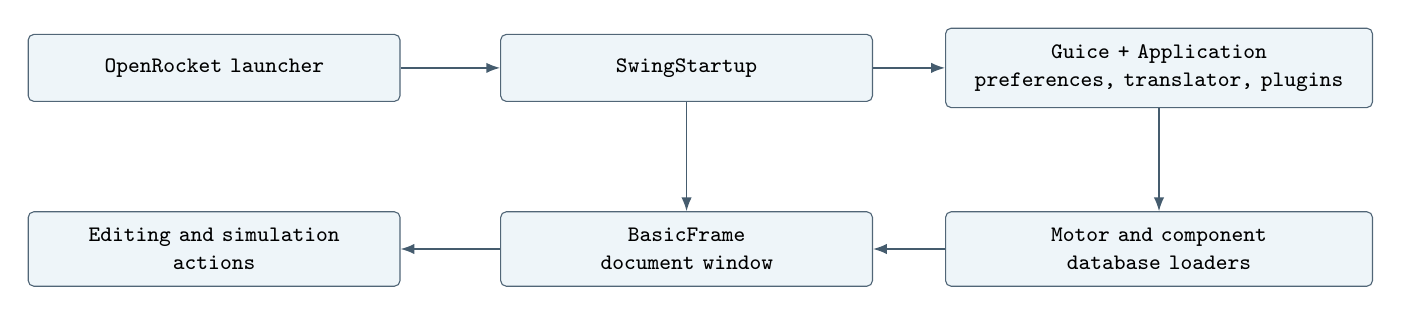
\begin{tikzpicture}
\simple{entry}{0,0}{OpenRocket launcher}{4.3cm}
\simple{start}{6,0}{SwingStartup}{4.3cm}
\simple{services}{12,0}{Guice + Application\\preferences, translator, plugins}{5cm}
\simple{load}{12,-2.3}{Motor and component\\database loaders}{5cm}
\simple{frame}{6,-2.3}{BasicFrame\\document window}{4.3cm}
\simple{work}{0,-2.3}{Editing and simulation\\actions}{4.3cm}
\draw[use] (entry) -- (start);
\draw[use] (start) -- (services);
\draw[use] (services) -- (load);
\draw[use] (start) -- (frame);
\draw[use] (load) -- (frame);
\draw[use] (frame) -- (work);
\end{tikzpicture}}

The MIT startup path adds its memory policy and repository-specific update routing. Those services are application maintenance concerns. They do not advance simulated time, choose controller outputs, or change the aerodynamic equations.

\section{Preferences, units, and localization}
\class{ApplicationPreferences} defines core-facing settings, while \class{SwingPreferences} supplies desktop persistence and UI preferences. Defaults for new simulations are distinct from the options saved with an existing simulation. Changing a global preference must not be assumed to rewrite every scenario already loaded.

The \code{unit} package separates storage/physics values from displayed units. Most physical values use SI internally: metres, kilograms, seconds, pascals, kelvin, and radians. \class{UnitGroup} collects compatible display choices; \class{Unit} performs conversion and formatting. Important exceptions and boundaries include degree-valued launch latitude/longitude, degree-valued FC commands, hPa/Celsius sensor adapters, and file fields whose saver/loader deliberately converts angles to degrees.

The \code{l10n} package supplies translations from resource bundles. UI labels are not stable identifiers. Persistence, component UUID mappings, controller source IDs, and event types should remain meaningful when the language or display name changes.

\section{Databases and presets}
Motor database services supply \class{ThrustCurveMotor} records and search/filter metadata. Loaders handle bundled motor resources and user-supplied thrust curves; the \code{thrustcurve} package contains online search/download support. A saved motor reference must resolve to an actual motor definition before flight calculations can use its curve and mass properties.

Component presets are catalog data used to populate components. \class{ComponentPreset}, typed property maps, XML DTOs, and database loaders manage dimensions, materials, and identifying metadata. Once instantiated, the rocket component is the editable design object. It is not a live remote catalog record. Property setters can clear preset associations when the component no longer matches its original preset.

Materials have different dimensional meanings: bulk density for volumes, surface density for sheets/canopies, and line density for cords. Treating all density fields as kilograms per cubic metre would produce incorrect masses. The selected component determines which material category and formula apply.

\section{Threading and service boundaries}
The Swing event-dispatch thread owns interactive widget updates. Simulations and long file/analysis operations use workers so the desktop remains responsive. Core objects such as \class{Simulation} and \class{RocketComponent} use safety checks, but those checks do not turn one shared mutable rocket into a concurrent simulation workspace. Batch and ensemble implementations create isolated copies for their workers.

Cancellation is cooperative: workers and listeners check interruption, then close their outputs. Result installation belongs to the coordinating workflow. In particular, an ensemble publishes a new result only after all required members complete successfully. This avoids relabeling a previous successful result as a partially completed new experiment.

\sourceline{\source{swing/src/main/java/info/openrocket/swing/startup/OpenRocket.java}{OpenRocket}; \source{swing/src/main/java/info/openrocket/swing/startup/SwingStartup.java}{SwingStartup}; \source{core/src/main/java/info/openrocket/core/startup/Application.java}{Application}; \source{core/src/main/java/info/openrocket/core/preferences/ApplicationPreferences.java}{ApplicationPreferences}; \source{core/src/main/java/info/openrocket/core/preset/ComponentPreset.java}{ComponentPreset}; \source{core/src/main/java/info/openrocket/core/database/MotorDatabaseLoader.java}{MotorDatabaseLoader}.}

\chapter{Documents, rocket components, and configurations}\label{ch:components}
\section{The document is the editing aggregate}
\class{OpenRocketDocument} groups a rocket with its simulations, custom expressions, storage options, appearance attachments, photo settings, undo history, and MIT motor-batch reports. The document is the natural unit for opening, saving, and presenting a design. A \class{Simulation} is a scenario owned by that document, not the document itself.

Document events inform views that simulations or other document-level data changed. Component events originate in the rocket tree. These two event systems overlap in user-visible effects but serve different owners. A new motor-batch report can dirty the document without changing a fin; a fin edit can invalidate aerodynamic data and simulation freshness while retaining the previous result for inspection.

\section{The component tree and class families}
Every design starts with a \class{Rocket} root. \class{RocketComponent} provides parent/child structure, identity, placement, naming, change notification, appearance, overrides, and common copy operations. Compatibility rules restrict which children belong under which parents. Assemblies organize stages and pods; physical component subclasses supply geometry and physical properties.

\begin{longtable}{@{}L{3cm}L{5.1cm}L{7cm}@{}}
\toprule Family & Representative classes & Role in the model\\\midrule\endhead
Assemblies & \class{Rocket}, \class{AxialStage}, \class{ParallelStage}, \class{PodSet} & Group children, define staging or repeated installations, and contribute instance transforms.\\
Outer airframe & \class{NoseCone}, \class{BodyTube}, \class{Transition} & Define external profiles, shell volume, wetted/projected geometry, and aerodynamic calculator selection.\\
Fin families & \class{TrapezoidFinSet}, \class{FreeformFinSet}, \class{EllipticalFinSet}, \class{TubeFinSet} & Describe outlines, count, placement, cant, thickness, and mass/aerodynamic geometry.\\
MIT control surfaces & \class{TabControlledTrapezoidFinSet}, \class{AirbrakeSet} & Add live tab angle or exposed fraction, corresponding physical coefficients, saving/loading, and editing/rendering support.\\
Internal/structural & \class{InnerTube}, \class{TubeCoupler}, \class{Bulkhead}, \class{CenteringRing}, \class{EngineBlock} & Model internal geometry, materials, mounting, and mass; internal parts need not create an external aerodynamic contribution.\\
Mass and support & \class{MassComponent}, \class{ShockCord}, \class{LaunchLug}, \class{RailButton} & Represent explicit mass, line-like components, and launch-guide hardware with their own geometry/drag behavior.\\
Recovery & \class{RecoveryDevice}, \class{Parachute}, \class{Streamer} & Store packed-component properties and deployment configuration; deployed drag is consumed by the recovery stepper.\\\bottomrule
\end{longtable}

A component can have a visible drawing without a separate aerodynamic contribution, and can have mass without being a surface exposed to the airflow. Conversely, turning off rendering visibility does not remove a component from simulation. These are deliberately different concerns.

\section{Placement, instances, and identity}
Axial placement uses an \class{AxialMethod} and offset relative to the parent/reference geometry. Radial and angular placement handle rings, fin sets, and off-axis assemblies. A tree node can represent several physical instances. \class{InstanceMap} and \class{InstanceContext} carry transformed occurrences so mass and aerodynamic calculations account for all installed copies.

This distinction matters for clustered motors, parallel boosters, and repeated fins. Counting tree nodes is not sufficient to count physical hardware. An individual fin contribution must not be multiplied once in a component calculator and then accidentally multiplied again when the active instances are traversed.

Components have UUIDs. Copies used to simulate or duplicate a scenario can preserve these IDs with \code{copyWithOriginalID()}, allowing saved mappings to resolve to the corresponding objects in the copied rocket. A new independently inserted component should have its own identity. Display names can change and are not a substitute for UUIDs. The FC block/recovery mappings use UUIDs; the Java named-output API deliberately uses exact unique names and checks for ambiguity.

\diagram{fig:document-configuration}{A design can support several motor/stage configurations and simulation scenarios. Each running branch derives its active physical configuration from the selected scenario.}{%
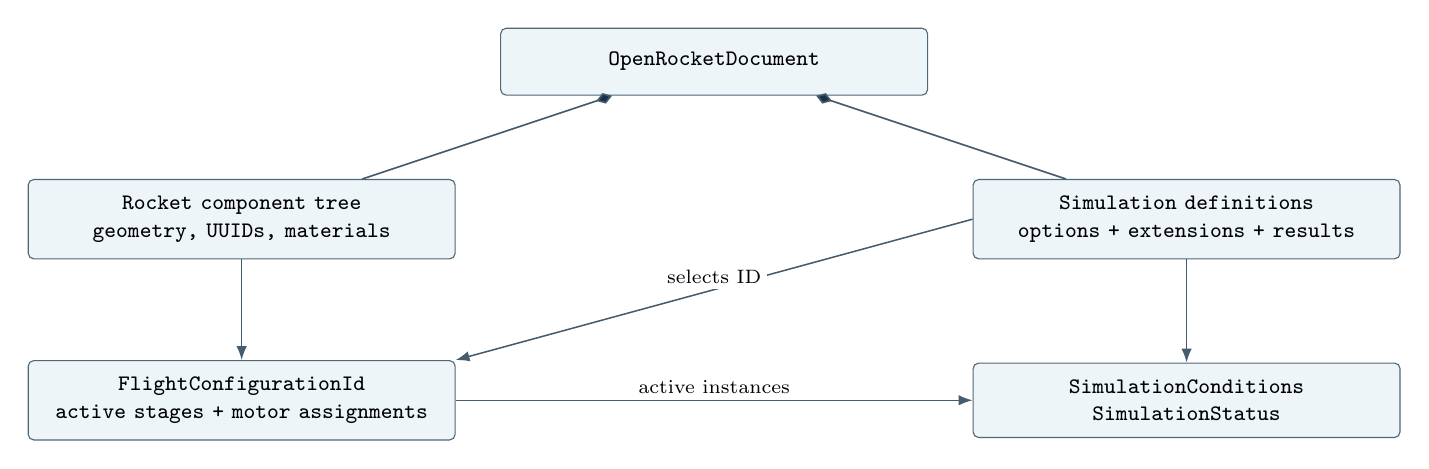
\begin{tikzpicture}
\simple{doc}{6,0}{OpenRocketDocument}{5cm}
\simple{rocket}{0,-2}{Rocket component tree\\geometry, UUIDs, materials}{5cm}
\simple{sims}{12,-2}{Simulation definitions\\options + extensions + results}{5cm}
\simple{fcfg}{0,-4.3}{FlightConfigurationId\\active stages + motor assignments}{5cm}
\simple{run}{12,-4.3}{SimulationConditions\\SimulationStatus}{5cm}
\draw[own] (doc) -- (rocket);
\draw[own] (doc) -- (sims);
\draw[use] (rocket) -- (fcfg);
\draw[use] (sims.west) -- node[flowlabel,above]{selects ID} (fcfg.north east);
\draw[use] (sims) -- (run);
\draw[use] (fcfg) -- node[flowlabel,above]{active instances} (run);
\end{tikzpicture}}

\section{A flight configuration is not a simulation option set}
\class{FlightConfiguration} associates a rocket with a configuration ID, stage activation, active components/instances, motor assignments, and reference dimensions. Flight-configurable component properties can vary by configuration: motors, ignition, stage separation, and recovery deployment settings are examples. \class{FlightConfigurableParameterSet} supplies the per-ID values and defaults.

\class{SimulationOptions} instead holds launch site, atmosphere/wind choices, rod settings, numerical settings, initial spin, and ensemble options. A simulation references one flight configuration and owns its own options. Several simulations can therefore compare weather or launch angles using the same installed motor configuration without duplicating the entire rocket design.

\section{Change propagation, overrides, and undo}
Geometry setters validate values and send \class{ComponentChangeEvent}s. Event categories distinguish changes that affect mass, aerodynamics, the component tree, or display. Modification identifiers and calculator caches use these signals to determine when derived data must be rebuilt. Bypassing setters can leave stale geometry, mass, or results even if a field contains the intended number.

Mass, CG, and drag overrides can apply to one component or a subtree. They are explicit modeling choices layered over calculated properties. A measured total mass override is not the same operation as changing every material density. Likewise, moving an overridden CG does not necessarily change the modeled shape or aerodynamic centre. The mass calculator and aerodynamic calculator interpret their own override flags.

Document undo records snapshots of the rocket at explicit undo points. GUI operations that transform a fin into a controlled fin must preserve appropriate geometry, materials, fillets, mounting tabs, and placement while making an undoable change. Simulation-dialog cancellation has a different snapshot lifecycle for options/extensions and prior results; it should not be treated as ordinary rocket-tree undo.

\section{Geometry and coordinate boundaries}
Component geometry uses a longitudinal model axis along X, increasing from the front toward the rear. Numerical flight integration uses a body frame with longitudinal Z and a quaternion relating it to the world frame. The 2D/3D design renderers have their own view transforms. In the MIT tab-preview work, the side-view model convention treats positive model Z as away from the observer. These conventions must be converted at the boundary; the same variable name does not imply the same axis across all subsystems.

Through-the-wall mounting tabs and aerodynamic roll-control tabs are separate features. Mounting tabs extend through the body to support the fin and affect structure/mass. Control tabs are deflected surfaces used by the MIT aerodynamic/control path. Adding a mounting tab does not create a controllable actuator.

\sourceline{\source{core/src/main/java/info/openrocket/core/rocketcomponent/RocketComponent.java}{RocketComponent}; \source{core/src/main/java/info/openrocket/core/rocketcomponent/FlightConfiguration.java}{FlightConfiguration}; \source{core/src/main/java/info/openrocket/core/rocketcomponent/FlightConfigurableParameterSet.java}{FlightConfigurableParameterSet}; \source{core/src/main/java/info/openrocket/core/rocketcomponent/InstanceMap.java}{InstanceMap}; \source{core/src/main/java/info/openrocket/core/document/OpenRocketDocument.java}{OpenRocketDocument}; \source{core/src/main/java/info/openrocket/core/rocketcomponent/TabControlledTrapezoidFinSet.java}{TabControlledTrapezoidFinSet}.}

\section{The complete native component vocabulary}\label{sec:catalogue}
The component tree is a parametric vehicle description. It supports the families below through concrete classes and shared placement/geometry interfaces. A mesh imported from a drawing program does not become an arbitrary new aerodynamic component. Freeform fins provide a custom two-dimensional planform; bodies remain members of the supported axisymmetric shape families. Assemblies combine these primitives into more complicated vehicles.

\subsection{Nose cones and all six body-profile families}
\class{NoseCone} specializes \class{Transition}: one end closes to the nose and the other joins the body. It supports flipping the orientation, an automatic or explicit base radius, length, shell thickness or solid fill, and a shoulder with its own dimensions and cap. The visible external contour, hidden shoulder, material volume, and aerodynamic reference volume have different roles.

The profile definitions live in \class{Transition.Shape}. For an untruncated nose, let $u=x/\ell$, where $x$ runs from tip to base, $\ell$ is length, $R$ is base radius, and $p$ is the shape parameter where present. These are geometry formulas; their aerodynamic treatments are discussed separately in Chapter~\ref{ch:aero}.

\begin{tabularx}{\linewidth}{@{}L{2.2cm}L{5.8cm}Y@{}}\toprule
Profile & Radius or construction & Parameter and interpretation\\\midrule
Conical & $r=Ru$ & Straight-sided cone or conical transition. No shape parameter.\\
Ogive & A circular-arc segment computed from length, radius, and $p$ & $p=1$ gives a tangent ogive; $0<p<1$ gives a secant ogive; the limit near zero becomes conical. Very short shapes use the source's scaling fallback.\\
Ellipsoid & $r=R\sqrt{2u-u^2}$ & Half-ellipse profile. Length and base radius set its axes; no shape parameter.\\
Power series & $r=Ru^p$ & $0\leq p\leq1$, default $1/2$. One gives a cone; values approaching zero become blunt, with a special numerical tip case.\\
Parabolic series & $r=R(2u-pu^2)/(2-p)$ & $p=0$ is conical, $p=1/2$ half-parabolic, $p=3/4$ three-quarter-parabolic, and $p=1$ full parabolic, tangent at the base.\\
Haack series & $r=R\sqrt{[\theta-\tfrac12\sin(2\theta)+p\sin^3\theta]/\pi}$, $\theta=\cos^{-1}(1-2u)$ & The exposed parameter range is $0$ to $1/3$. Zero is LD-Haack/von K\'arm\'an; $1/3$ is LV-Haack. These shape names do not establish minimum drag for every installed transition or flight condition.\\\bottomrule
\end{tabularx}

\diagram{fig:body-profile-path}{One radius function supplies several independent products. Material properties and aerodynamic shape properties must not be conflated.}{
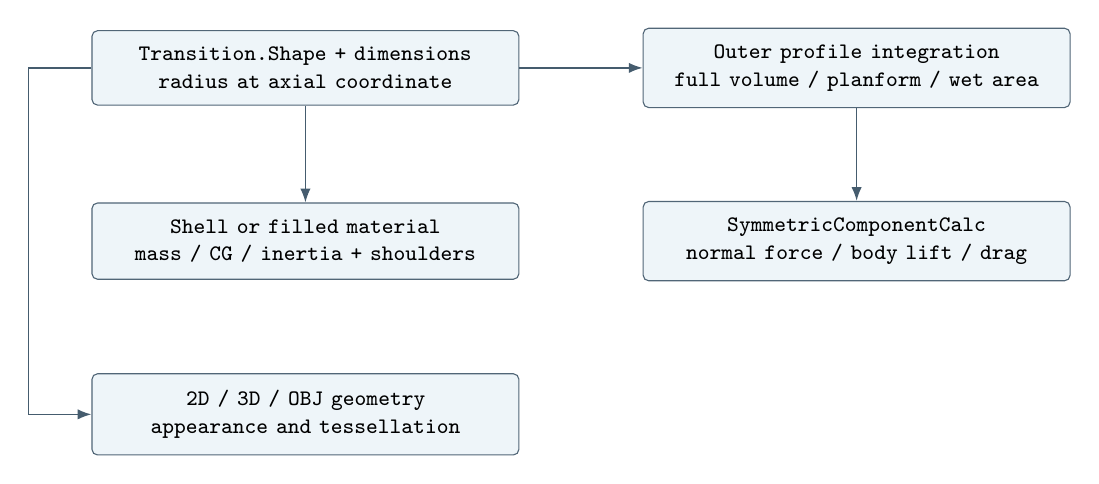
\begin{tikzpicture}
\simple{shape}{0,0}{Transition.Shape + dimensions\\radius at axial coordinate}{5cm}
\simple{outer}{7,0}{Outer profile integration\\full volume / planform / wet area}{5cm}
\simple{mass}{0,-2.2}{Shell or filled material\\mass / CG / inertia + shoulders}{5cm}
\simple{aero}{7,-2.2}{SymmetricComponentCalc\\normal force / body lift / drag}{5cm}
\simple{draw}{0,-4.4}{2D / 3D / OBJ geometry\\appearance and tessellation}{5cm}
\draw[use] (shape)--(outer); \draw[use] (shape)--(mass);
\draw[use] (outer)--(aero); \draw[use] (shape.west) -- ++(-.8,0) |- (draw.west);
\end{tikzpicture}}

\subsection{Transitions, boattails, and shoulders}
A \class{Transition} joins independently specified fore and aft radii. Increasing radius gives an expanding transition; decreasing radius gives a boattail. The same shape family can be applied in the reversed axial direction. For clippable families, a clipped transition selects a segment of a longer parent shape so its front has the requested nonzero radius. An unclipped transition offsets/scales the profile between its two radii. This changes the actual contour, so it can change material volume, wetted area, pressure drag, and CP.

Fore and aft shoulders are insertion geometry used for fit and mass. Their radius, length, thickness, and optional caps contribute through the component's structural calculations. They are not automatically treated as separate exposed nose cones by the aerodynamic calculator. Neighbor searches support automatic radii and identify adjoining exterior bodies. An incorrect axial gap, overlap, or radius discontinuity can therefore affect both warnings and exposed-area drag.

\sourceline{\source{core/src/main/java/info/openrocket/core/rocketcomponent/NoseCone.java}{NoseCone}; \source{core/src/main/java/info/openrocket/core/rocketcomponent/Transition.java}{Transition and Shape}; \source{core/src/main/java/info/openrocket/core/rocketcomponent/SymmetricComponent.java}{SymmetricComponent}.}

\subsection{Body tubes and internal cylindrical parts}
\class{BodyTube} is an exposed constant-radius shell with length, outer radius, thickness/inner radius, material, finish, appearance, and motor-mount capability. A cylindrical tube has no area-change Barrowman normal-force term, but it still contributes skin friction, finite-angle body lift, and exposed-end drag. An internal void changes structural mass; it is not a simulated duct through the main rocket body.

\class{InnerTube} is an internal tube that can be a motor mount and can be repeated in a cluster. \class{TubeCoupler} represents an internal joining sleeve. \class{CenteringRing} and \class{Bulkhead} represent annular and solid supporting plates; \class{EngineBlock} represents an internal stop ring. Shared ring bases distinguish specifying radii directly from specifying wall thickness, and some automatic dimensions fit the parent tube or enclosed motor-mount geometry. These parts contribute mass and inertia but are not independently exposed surfaces in the normal ascent aerodynamic calculation.

The \class{Tube}, \class{Coaxial}, \class{RadialParent}, and positioning interfaces express geometry capabilities used by multiple classes. Their existence does not mean that a user can insert the interface itself as a new part. Likewise, \class{BodyComponent}, \class{StructuralComponent}, and \class{InternalComponent} are shared implementation layers.

\sourceline{\source{core/src/main/java/info/openrocket/core/rocketcomponent/BodyTube.java}{BodyTube}; \source{core/src/main/java/info/openrocket/core/rocketcomponent/InnerTube.java}{InnerTube}; \source{core/src/main/java/info/openrocket/core/rocketcomponent/TubeCoupler.java}{TubeCoupler}; \source{core/src/main/java/info/openrocket/core/rocketcomponent/CenteringRing.java}{CenteringRing}; \source{core/src/main/java/info/openrocket/core/rocketcomponent/Bulkhead.java}{Bulkhead}; \source{core/src/main/java/info/openrocket/core/rocketcomponent/EngineBlock.java}{EngineBlock}.}

\subsection{Trapezoidal, elliptical, and freeform fins}
\class{TrapezoidFinSet} describes root chord, tip chord, span, and sweep. Choosing equal chords and zero sweep gives a rectangular planform; setting a zero tip chord gives a triangular planform. These are parameter choices within one component family. \class{EllipticalFinSet} defines an elliptical outline using root chord and span. \class{FreeformFinSet} stores an editable sequence of outline points, with validation and point-editing operations. The point sequence is a planar fin contour, not a general 3D airfoil definition.

All inherit \class{FinSet}'s count, angular orientation, axial placement, thickness, material, cross section, cant, mounting tab, and fillet properties. Their geometry is ultimately exposed as fin/root points and planform measures for calculators and renderers. Root geometry can follow the supporting body. A fin with more elaborate outline points still enters the same strip-based aerodynamic approximation; unsupported concavities or jagged edges can generate warnings.

The native cross-section categories are square, rounded, and airfoil; this fork adds triangular leading edges. They select specific geometric-volume factors and pressure-drag treatments. In the source, the baseline volume factors are 1.00, 0.99, and 0.85 respectively. ``Airfoil'' is a generic category, not an imported NACA profile or a Reynolds-dependent polar table. The triangular category has its own bevel/volume handling in the MIT implementation.

Through-the-wall tabs and fillets supply structural geometry. Fin material mass, tab mass, and fillet material mass are accumulated with their centroids. The ordinary tab below the body surface is distinct from an exposed control tab. A fillet can alter mass and the rendered root without implying a dedicated CFD-derived fillet/interference drag model. Cant changes the installed incidence and roll forcing; moving a fin axially changes the CP lever arm even if its planform is unchanged.

\sourceline{\source{core/src/main/java/info/openrocket/core/rocketcomponent/TrapezoidFinSet.java}{TrapezoidFinSet}; \source{core/src/main/java/info/openrocket/core/rocketcomponent/EllipticalFinSet.java}{EllipticalFinSet}; \source{core/src/main/java/info/openrocket/core/rocketcomponent/FreeformFinSet.java}{FreeformFinSet}; \source{core/src/main/java/info/openrocket/core/rocketcomponent/FinSet.java}{FinSet}.}

\subsection{Tube fins and launch hardware}
\class{TubeFinSet} repeats cylindrical ring fins around a parent body. Length, radius, wall thickness, count, and angular position define both the tubes and the gaps between them. The aerodynamic model assumes zero tube cant and uses ring-airfoil and tube-flow approximations. Separated, overlapping, or isolated tubes are specifically diagnosed; they are not all equivalent to a conventional planar fin set.

\class{LaunchLug} is a small external guide tube, with tube geometry, placement, and repetition. Its calculator includes internal-flow and end-pressure drag, while neglecting separate skin friction and nonaxial forces. \class{RailButton} has flange/body dimensions, height, placement, and repeated instances; its drag model accounts approximately for the local boundary layer. The launch-status calculation uses launch-lug positions to establish effective guide travel; the inspected correction does not include rail buttons. Neither component models contact stress or guide friction dynamically.

\subsection{Mass objects, cords, and recovery devices}
\class{MassComponent} represents payload, electronics, ballast, or another explicitly specified mass with placement and a display envelope. Its type can affect its label or drawing without adding a new physical subsystem. It is useful when detailed construction is unnecessary, but a mass lump does not become an external aerodynamic shape merely by resembling one visually.

\class{ShockCord} uses line density and cord length for mass, with packed placement in the rocket. \class{Parachute} and \class{Streamer} use sheet-area and, for parachutes, suspension-line properties. Their packed envelopes serve design placement; their deployed areas and coefficients belong to recovery simulation. The recovery rules and descent force laws are explained in Chapter~\ref{ch:recovery}.

\sourceline{\source{core/src/main/java/info/openrocket/core/rocketcomponent/TubeFinSet.java}{TubeFinSet}; \source{core/src/main/java/info/openrocket/core/rocketcomponent/LaunchLug.java}{LaunchLug}; \source{core/src/main/java/info/openrocket/core/rocketcomponent/RailButton.java}{RailButton}; \source{core/src/main/java/info/openrocket/core/rocketcomponent/MassComponent.java}{MassComponent}; \source{core/src/main/java/info/openrocket/core/rocketcomponent/ShockCord.java}{ShockCord}.}

\section{Assemblies, clusters, and reference dimensions}
\class{Rocket} is the root aggregate. \class{AxialStage} groups components that belong to one axial stage. \class{ParallelStage} represents repeated detachable side stages, and \class{PodSet} groups offset components without making every pod a separate powered flight stage. The assembly itself is primarily an organizational and transformation object; its descendants supply geometry and physical properties. An assembly can nevertheless carry aggregate overrides.

Ring/line instances specify repeated positions and orientations. \class{ClusterConfiguration} defines motor-tube patterns, with cluster scale and rotation supplied by the tube. Parent and child instance transforms compose, so a multi-motor mount repeated on several boosters yields more physical motors than the number of tree nodes suggests. Stage activity affects the active instance map used for reference area, mass, aerodynamics, motor state, and result branches.

Reference dimensions are selected by \class{ReferenceType}. The nose-based option uses the first qualifying nonzero symmetric-body diameter; the maximum option uses the largest active symmetric-body end diameter; the custom option uses the rocket's explicitly chosen reference length. The reference area is circular, $S=\pi D_{\rm ref}^2/4$. This is the normalization for coefficients and caliber stability, not necessarily the largest arbitrary mesh projection. A reference change can alter a coefficient's numeric value without an equivalent change in the dimensional force.

\sourceline{\source{core/src/main/java/info/openrocket/core/rocketcomponent/ParallelStage.java}{ParallelStage}; \source{core/src/main/java/info/openrocket/core/rocketcomponent/PodSet.java}{PodSet}; \source{core/src/main/java/info/openrocket/core/rocketcomponent/ClusterConfiguration.java}{ClusterConfiguration}; \source{core/src/main/java/info/openrocket/core/rocketcomponent/ReferenceType.java}{ReferenceType}.}


\chapter{Mass, propulsion, atmosphere, and reference frames}\label{ch:models}
The flight engine does not calculate every physical property itself. It asks separate model objects for mass, motor thrust, atmosphere, wind, gravity, and aerodynamic coefficients. \class{SimulationConditions} brings these services together for one scenario. \class{AbstractSimulationStepper} provides common evaluation methods and the pre/post listener hooks around them.

\section{Mass properties and rigid-body aggregation}
Component classes calculate local mass and centre of mass from geometry and materials. \class{MassCalculation} traverses the active configuration and its instances, translates local centres into assembly coordinates, respects applicable overrides, and aggregates the contributions. \class{MassCalculator} exposes convenient entry points for structure, launch, burnout, and time-dependent motor mass. \class{RigidBody} carries the resulting mass, centre, and inertias.

For ordinary contributions, the conceptual aggregation is
\begin{equation}
 m=\sum_i m_i,\qquad \boldsymbol r_{CG}=\frac{\sum_i m_i\boldsymbol r_i}{m},
 \qquad I=\sum_i\left(I_i+m_i d_i^2\right),
\end{equation}
with the appropriate axis and transformed instance positions. Overrides alter which contributions are included and how they are represented; they must be inspected before applying this expression to a particular design. The implementation distinguishes inertia about the longitudinal spin axis from transverse/pitch inertia. The flight stepper uses these effective inertias rather than a general deformable-body model.

Structure and motor contributions are evaluated separately. The structure normally remains constant within an unchanging active-stage configuration, while motor mass/CG follow motor time and stage activity. Staging changes the active set. A simulation actuator can also trigger component changes through the normal model API. Caches and change identifiers must therefore be consistent with both static design edits and supported live actuator properties.

\section{Motor data, installation, and ignition state}
\class{Motor} describes a motor model. \class{ThrustCurveMotor} supplies sampled thrust, mass/CG information, dimensions, manufacturer/designation metadata, and supported delays. It interpolates time-series values from the stored curve. The numerical integrator can evaluate a curve at intermediate Runge--Kutta stages; the motor is not advanced by incrementing a mutable sample index.

\class{MotorConfiguration} describes installation in a mount for a flight configuration, including ignition behavior and ejection delay. \class{MotorClusterState} is the per-run state for that installation: armed, thrusting, delaying, or spent, with actual ignition/cutoff/ejection times. Motor time is measured relative to ignition. Cluster count comes from the mount's physical instances and scales thrust appropriately.

The engine schedules ignition, burnout, and ejection events. An ejection charge is an event source that can activate ordinary recovery rules; it is not itself a deployed parachute. Plugged motors do not create the same ejection path. The MIT engine also schedules thrust-curve sample boundaries; FC-aware timing uses ignition-relative offsets so delayed ignition does not shift the curve into the wrong clock frame.

RASP \code{.eng} and RockSim motor loaders populate the motor database separately from rocket geometry. Unresolved references can generate loading warnings. Reproducibility requires curve identity/data and delay, not just a motor display label.

\section{Atmosphere and gravity}
\class{AtmosphericModel} returns \class{AtmosphericConditions} at altitude. The standard implementation, \class{ExtendedISAModel}, supports a layered ISA-derived atmosphere anchored either to standard conditions or custom launch pressure and temperature. It inherits interpolation support from \class{InterpolatingAtmosphericModel}. Atmospheric conditions supply density, sound speed, and viscosity-related quantities used by the aerodynamic path.

Pressure is in pascals and temperature in kelvin in the physical atmosphere. The FC adapter deliberately converts those values to hPa and Celsius. Launch altitude is mean-sea-level altitude; trajectory height above the pad is a different quantity. A pressure-derived barometric height zeroed during preflight is different again. These distinctions matter when comparing recorded telemetry with simulator truth.

\class{GravityModel} supplies gravity at a world location; \class{WGSGravityModel} is the normal implementation. \class{GeodeticComputationStrategy} converts local displacements to world coordinates and supplies the appropriate Coriolis term for the selected strategy. Flat, spherical, and other provided strategies are model choices, not display-only options.

\section{Wind and stochastic inputs}
\class{WindModel} is queried by time and altitude and can use MSL or AGL altitude references. \class{PinkNoiseWindModel} represents a baseline wind with correlated turbulence. \class{MultiLevelPinkNoiseWindModel} supports altitude-dependent profiles. Seeds are part of reproducibility: changing unrelated evaluation order should not casually introduce new random draws into a physical model.

The stepper constructs its relative-airflow vector using the wind model's convention. In the inspected code this calculation is \code{rocketVelocity.add(windVelocity)}, followed by rotation into the body frame. An external wind-vector source must be adapted to this convention rather than substituted under an assumed textbook sign. Bearing is clockwise from north; world horizontal axes are east and north.

Ensemble wind variation is layered onto these models: a per-flight bearing rotation and east/north offsets modify the existing profile while the baseline turbulence seed remains fixed across members. This is distinct from FC sensor noise, which perturbs the observations of the resulting flight.

\section{Coordinate and unit contracts}
\begin{tabularx}{\linewidth}{@{}L{3.3cm}YY@{}}\toprule
Boundary & Convention & Consequence\\\midrule
Component geometry & Longitudinal model X; placement relative to parent/assembly & CP and CG axial coordinates are model positions, not world altitude.\\
Flight world & X east, Y north, Z upward & Trajectory translation and world angular vectors use this frame.\\
Flight body & Longitudinal Z; quaternion maps body to world & Thrust, rotational rates, and sensor adapters require explicit transforms.\\
FC sensor mounting & Baseline X = body Z, Y = body X, Z = body Y & Longitudinal acceleration feeds sensor X; roll integration uses negative sensor X rate.\\
Display and persistence & Unit-group conversions; some file angles stored in degrees & Never copy displayed values directly into radian-valued setters.\\\bottomrule
\end{tabularx}

\begin{contract}
These are rigid-body engineering models, without fluid-structure, combustion, flexible-body, or complete electronics dynamics. A replacement submodel must preserve units, frames, timing, and listener contracts.
\end{contract}
\sourceline{\source{core/src/main/java/info/openrocket/core/masscalc/MassCalculation.java}{MassCalculation}; \source{core/src/main/java/info/openrocket/core/masscalc/RigidBody.java}{RigidBody}; \source{core/src/main/java/info/openrocket/core/motor/ThrustCurveMotor.java}{ThrustCurveMotor}; \source{core/src/main/java/info/openrocket/core/simulation/MotorClusterState.java}{MotorClusterState}; \source{core/src/main/java/info/openrocket/core/models/atmosphere/ExtendedISAModel.java}{ExtendedISAModel}; \source{core/src/main/java/info/openrocket/core/util/GeodeticComputationStrategy.java}{GeodeticComputationStrategy}.}

\section{How shape becomes mass, CG, and inertia}
For a constant-radius hollow tube, the structural volume is conceptually $\pi(r_o^2-r_i^2)\ell$, multiplied by bulk material density. Its CG lies halfway along its uniform length, and hollow-cylinder inertia formulas distinguish rotation about the long axis from rotation about a transverse axis. Internal rings use the same kind of volume accounting with their own dimensions. A mass object instead supplies explicit mass and an approximate envelope for inertia.

Curved \class{SymmetricComponent} shapes use 128 axial divisions. At each division the code evaluates the external radius at both ends and treats the segment as a conical frustum. A hollow shell subtracts an inner frustum, using wall slope to convert specified thickness into radial material depth; a filled component uses zero inner radii. Segment volumes, first moments, and axial/transverse inertias are accumulated, followed by the parallel-axis shift to the component CG.

The same traversal separately accumulates full external volume, wetted surface area, side-projected planform area, and planform centroid. Full volume describes the outer shape regardless of whether the part is hollow. It is used in aerodynamic CP relationships. Material volume describes what is actually made of the selected material. Substituting one for the other would make a hollow nose's aerodynamic CP incorrectly depend on its wall thickness.

Fin properties are reduced from the outline and supporting root. Material volume includes the profile's thickness factor; mounting tabs and fillets add their own volumes and centroids. Repeated fins, rings of pods, and motor clusters require transformed instance locations before aggregation. Moving a component sideways or rotating an assembly can affect inertia even if total mass and axial CG barely change.

Mass and CG overrides operate at their selected scope. A component-only mass override retains its children as separate contributions. A subtree mass override suppresses the children's aggregate mass contribution; a subtree CG override relocates the children's aggregate center according to the code's override semantics. Unit-inertia approximations remain tied to component geometry. These options are useful for reconciling a measured vehicle, but they are not a procedure for identifying a full measured inertia tensor.

\sourceline{\source{core/src/main/java/info/openrocket/core/rocketcomponent/SymmetricComponent.java}{calculateProperties}; \source{core/src/main/java/info/openrocket/core/rocketcomponent/FinSet.java}{fin mass, tabs, and fillets}; \source{core/src/main/java/info/openrocket/core/masscalc/MassCalculation.java}{structure/motor traversal and overrides}; \source{core/src/main/java/info/openrocket/core/masscalc/MassCalculator.java}{mass calculation entry points}.}

\section{Motor curves, propulsion timing, and database identity}
A thrust-curve motor stores paired time/thrust samples and mass/CG information. \class{ThrustCurveMotor} locates the surrounding sample interval and linearly interpolates thrust and center-of-mass data at the requested motor time. The same object can be queried at several provisional solver times without changing its state. Calculated metadata such as total impulse, average thrust, maximum thrust, and estimated burn duration supports selection and reporting; the designation is not a replacement for the curve.

Loaders handle the different information available in RASP and RockSim motor formats. They validate and normalize input, and may derive mass evolution when the source lacks a full measured mass history. Manufacturer normalization, motor digests, curve sets, and the database finder help distinguish similar names and alternate measurements. A nominal ``same motor'' selection can still refer to different curve data, so reproduction should retain the actual resolved identity.

The installation's \class{IgnitionEvent} can be launch, the lower stage's ejection or burnout, automatic, or never, with an additional configured delay. Automatic selects launch for a launch stage and ejection-triggered ignition for an upper stage. The running \class{MotorClusterState} tracks when that condition actually occurred. A motor's thrust and remaining mass use elapsed time since its own ignition, while the flight branch uses simulation time. Delay/ejection and stage separation are distinct event paths.

Thrust is summed over active motor installations and their physical instances. The model reads supplied thrust curves; it does not solve chamber pressure, nozzle flow, combustion instability, or an electrical ignition circuit. A cluster configuration repeats motor geometry and thrust; it does not imply a modeled ignition-failure distribution unless an explicit extension supplies one.

\sourceline{\source{core/src/main/java/info/openrocket/core/motor/ThrustCurveMotor.java}{ThrustCurveMotor}; \source{core/src/main/java/info/openrocket/core/motor/IgnitionEvent.java}{IgnitionEvent}; \source{core/src/main/java/info/openrocket/core/database/motor/ThrustCurveMotorSet.java}{ThrustCurveMotorSet}; \source{core/src/main/java/info/openrocket/core/simulation/MotorClusterState.java}{MotorClusterState}.}

\section{Atmospheric quantities used by the solver}
The atmosphere supplies pressure and temperature; \class{AtmosphericConditions} derives dry-air density as $\rho=P/(RT)$ with $R=287.053\ \mathrm{J\,kg^{-1}K^{-1}}$. In this implementation the sound speed is the linear approximation $a=165.77+0.606T$ in m/s, with $T$ in kelvin. Kinematic viscosity is $(3.7291\times10^{-6}+4.9944\times10^{-8}T)/\rho$. It is therefore inaccurate to describe this code as evaluating the exact ideal-gas sound-speed expression or full Sutherland viscosity at every sample.

\class{ExtendedISAModel} uses layer boundaries at 0, 11, 20, 32, 47, 51, 71, and 84.852 km, with prescribed base temperatures and hydrostatic pressure relations. Custom launch conditions anchor the lower atmosphere and connect to the higher layer structure. Its constructor restricts a custom first altitude to below 11 km and validates positive absolute temperature and pressure. An interpolation wrapper caches sampled atmospheric values for repeated queries.

The standalone \class{AtmosphericConditions} default is 293.15 K, whereas the standard \class{ExtendedISAModel} sea-level baseline is 288.15 K. Code that constructs a fresh conditions object for a static analysis is not necessarily using the same atmosphere as a flight simulation at its configured launch site. The source also records known approximation limits at high altitude. Humidity, precipitation, and detailed meteorological assimilation are not modeled by these classes.

\section{Wind profiles, gravity, and Earth geometry}
The average wind model combines mean speed/direction with seeded correlated pink-noise turbulence. Turbulence intensity and standard deviation describe variability around the mean; they are not a sequence of independent draws at each RK evaluation. The multilevel model stores altitude-dependent wind levels and interpolates profile behavior, with an explicit AGL/MSL altitude reference. Wind-profile import and editing prepare this model before execution.

Gravity uses a latitude-dependent WGS-style surface magnitude and an inverse-square altitude correction. The geodetic strategy separately controls how local displacement becomes geographic position: \code{FLAT} uses meters-per-degree scaling and zero Coriolis acceleration; \code{SPHERICAL} uses great-circle geometry; \code{WGS84} uses an ellipsoid/Vincenty direct solution. The latter two include the implementation's Coriolis term. Selecting a more detailed map geometry does not replace the rest of the force model.

\sourceline{\source{core/src/main/java/info/openrocket/core/models/atmosphere/AtmosphericConditions.java}{AtmosphericConditions}; \source{core/src/main/java/info/openrocket/core/models/atmosphere/InterpolatingAtmosphericModel.java}{InterpolatingAtmosphericModel}; \source{core/src/main/java/info/openrocket/core/models/wind/PinkNoiseWindModel.java}{PinkNoiseWindModel}; \source{core/src/main/java/info/openrocket/core/models/wind/MultiLevelPinkNoiseWindModel.java}{MultiLevelPinkNoiseWindModel}; \source{core/src/main/java/info/openrocket/core/models/gravity/WGSGravityModel.java}{WGSGravityModel}.}


\chapter{Aerodynamics: bodies, fins, drag, and control surfaces}\label{ch:aero}
\section{Calculator boundary}
\class{AerodynamicCalculator} separates force modeling from integration. It consumes a \class{FlightConfiguration} and \class{FlightConditions}, and produces \class{AerodynamicForces}, optionally with warnings and per-component analyses. The normal calculator is \class{BarrowmanCalculator}, an extended engineering model with component-specific calculations and empirical corrections across its supported regimes.

\class{FlightConditions} packages relative speed, Mach number, angle of attack, lateral flow direction, rotation rates, atmospheric properties, and reference geometry. \class{AerodynamicForces} packages nondimensional coefficients, CP, and force/moment-related quantities. A calculator does not directly move the rocket; the stepper converts these coefficients into dimensional accelerations.

\diagram{fig:aerodynamics}{The aerodynamic path separates flight conditions, component calculations, and integration. Cached geometry and live actuator values have different update requirements.}{%
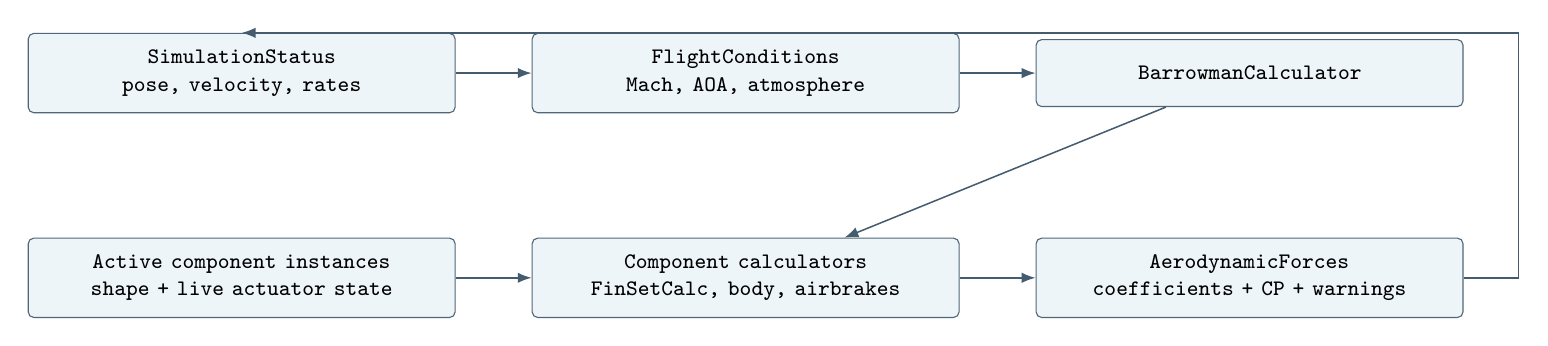
\begin{tikzpicture}
\simple{status}{0,0}{SimulationStatus\\pose, velocity, rates}{5cm}
\simple{conditions}{6.4,0}{FlightConditions\\Mach, AOA, atmosphere}{5cm}
\simple{calc}{12.8,0}{BarrowmanCalculator}{5cm}
\simple{geometry}{0,-2.6}{Active component instances\\shape + live actuator state}{5cm}
\simple{parts}{6.4,-2.6}{Component calculators\\FinSetCalc, body, airbrakes}{5cm}
\simple{forces}{12.8,-2.6}{AerodynamicForces\\coefficients + CP + warnings}{5cm}
\draw[use] (status) -- (conditions);
\draw[use] (conditions) -- (calc);
\draw[use] (calc) -- (parts);
\draw[use] (geometry) -- (parts);
\draw[use] (parts) -- (forces);
\draw[use] (forces.east) -- ++(.7,0) |- (status.north);
\end{tikzpicture}}

\section{Component decomposition and caching}
The calculator maintains a mapping from components to classes in \code{aerodynamics.barrowman}, generally using the component type and a \code{Calc} suffix. Body shapes, fin sets, tube fins, rail buttons, launch lugs, and airbrakes have different geometric contributions. Active-instance transforms ensure repeated/off-axis installations participate in the assembled result.

Geometry such as fin planform, mean aerodynamic chord, span, and wetted surface can be cached. The calculator checks modification IDs to invalidate those caches after design changes. Live actuator state is different: the MIT \class{FinSetCalc} reads tab deflection and fin cant on each force calculation, including when the geometric cache survives a PWM update. A cached constructor-time angle would disconnect a controller from the physics despite apparently correct servo logs.

Drag is assembled from the model's friction, pressure, base, and override contributions. Surface finish, dimensions, Reynolds/Mach-dependent relationships, and fin cross section influence relevant terms. CP and normal-force derivatives come from the assembled component calculations. A renderer's outline is not the aerodynamic model: making a rounded edge visually smooth does not itself alter these coefficients.

\section{Force and moment normalization}
Using dynamic pressure \(q=\tfrac12\rho V^2\), reference area \(S\), and reference length \(L\), a typical dimensional coefficient relationship is
\begin{equation}
 F=qSC_F,\qquad M=qSLC_M.
\end{equation}
The stepper applies the implementation's axial/lateral signs and frame rotations. Pitch/yaw moments are shifted from the model reference origin to the current mass centre using the associated force coefficients. A change in CG can therefore change angular response even when geometry and aerodynamic coefficients remain unchanged.

Fin cant supplies roll forcing, while roll-rate-dependent terms supply damping. The net roll coefficient is forcing minus damping. This separation is preserved by the MIT ensemble coefficient variations so uncertainty in forcing does not accidentally become uncertainty in the opposing term as well.

\section{How the inherited drag budget is assembled}\label{sec:drag-budget}
The normal calculation evaluates nonaxial component forces, then computes four drag terms:
\begin{equation}
C_D=C_{D,\mathrm{friction}}+C_{D,\mathrm{pressure}}+
C_{D,\mathrm{base}}+C_{D,\mathrm{override}}.
\end{equation}
Friction is viscous drag along wetted surfaces. Pressure drag includes nose/transition profiles, fin edges, exposed steps, and hardware-specific losses. Base drag accounts for exposed rear-facing body area. An override substitutes a specified contribution for the calculated drag of the selected component or subtree. Contributions are normalized to the same rocket reference area and multiplied by the appropriate physical instance counts.

This budget is not an arbitrary mesh surface integration. Each supported class selects a calculator with a particular approximation. An exposed body shoulder is handled differently from a fin leading edge, a hollow launch lug, or a deployed parachute. Internal centering rings and payload masses do not enter this budget as independent external surfaces. Aerodynamic area, structural material area, and drawing area must therefore remain separate concepts.

\section{Skin friction, Reynolds number, and surface finish}
The whole-vehicle Reynolds number used for the baseline skin-friction coefficient is
\begin{equation}
Re=\frac{V\ell_{\rm aero}}{\nu},
\end{equation}
where $\ell_{\rm aero}$ is the active aerodynamic length and $\nu$ is kinematic viscosity. The standard fully turbulent branch uses $C_f=0.0148$ below $Re=10^4$ and
\begin{equation}
C_f=\frac{1}{(1.50\ln Re-5.6)^2}
\end{equation}
above it, before compressibility and roughness corrections. The logarithm in this expression is natural. This is not a per-fin Reynolds-number calculation based on each fin's chord.

The rocket's perfect-finish option enables a partly laminar model: $C_f=0.0133$ at very low Reynolds number, $1.328/\sqrt{Re}$ from $10^4$ to $5.39\times10^5$, and the turbulent expression minus $1700/Re$ above that threshold. Mach corrections use different subsonic and supersonic formulas and interpolate across Mach 0.9--1.1. In the ordinary turbulent branch, the low-Mach factor is $1-0.1M^2$ and the high-Mach factor is $(1+0.15M^2)^{-0.58}$.

Each external component's finish supplies a roughness height $k$. A second estimate is
\begin{equation}
C_{f,\mathrm{rough}}=0.032\left(\frac{k}{\ell_{\rm aero}}\right)^{0.2}R(M),
\end{equation}
where $R$ is the source's Mach-dependent roughness correction. The ordinary branch takes the maximum of smooth/turbulent and roughness-limited estimates. Perfect finish only permits the roughness limit to dominate above $Re=10^6$. Thus a smoother-looking appearance texture does not reduce drag; the physical finish setting does.

\begin{tabularx}{\linewidth}{@{}L{4cm}L{2.2cm}Y@{}}\toprule
Finish category & $k$ in $\mu$m & Interpretation\\\midrule
Rough / rough unfinished & 500 / 250 & Large surface roughness\\
Unfinished / regular paint & 150 / 60 & Ordinary unfinished and painted surfaces\\
Smooth / optimum paint & 20 / 5 & Smaller prescribed roughness\\
Aircraft sheet metal & 2 & Internal enum name \code{POLISHED} retained for compatibility\\
Polished / mirror & 0.5 / 0 & \code{FINISHPOLISHED} and \code{MIRROR}; mirror still has the smooth-wall friction term\\\bottomrule
\end{tabularx}

Symmetric bodies contribute $C_f A_{\rm wet}/S$. The assembly applies an additional body slenderness factor $1+1/(2f_B)$, with the implementation's $f_B$ based on the active body's axial extent divided by its maximum radius. Fins instead use their own thickness correction. The two factors should not be applied twice when recreating a component breakdown outside the application.

\sourceline{\source{core/src/main/java/info/openrocket/core/aerodynamics/BarrowmanCalculator.java}{calculateFrictionCD / calculateFrictionCoefficient}; \source{core/src/main/java/info/openrocket/core/rocketcomponent/ExternalComponent.java}{Finish}.}

\section{Nose-cone and expanding-transition pressure drag}
\class{SymmetricComponentCalc} uses the geometry's end radii, length, full external volume, planform, wetted area, and shape parameter. It normalizes the nose/transition pressure coefficient by
\begin{equation}
\frac{A_{\rm frontal}}{S}=\frac{\pi|r_{\rm aft}^2-r_{\rm fore}^2|}{S}.
\end{equation}
An equal-radius body segment has no profile pressure-drag term in this method. A segment shorter than 1 mm uses a blunt-step approximation. For a longer expanding profile, the calculator builds and caches a Mach-to-pressure-coefficient interpolator.

Conical and ogive profiles use analytical/empirical relations. The conical path is the zero-ogive-parameter case. Between Mach 1 and 1.3, a polynomial joins endpoint values and derivatives. Above Mach 1.3, the constructed table uses
\begin{equation}
C_{D,p}^{*}=\bigl[0.72(p-0.5)^2+0.82\bigr]
\left(2.1\sin^2\phi+\frac{0.5\sin\phi}{\sqrt{M^2-1}}\right),
\end{equation}
where $p$ is the ogive parameter and $\sin\phi$ is derived from the aft profile slope. The star denotes the local coefficient before frontal-area normalization. The code builds this table through approximately Mach 4; its interpolator behavior outside tabulated ranges is not a new high-Mach validation.

Ellipsoid, power-series, parabolic, and Haack profiles use embedded experimental coefficient tables for fineness ratio 3. Parameterized profiles interpolate between bounding shape tables: power-series examples include exponents $1/4$, $1/2$, and $3/4$; parabolic examples include half, three-quarter, and full parabola; Haack uses von K\'arm\'an and LV-Haack tables. The source identifies the historical data origin in its comments. The application does not call an external aerodynamic database during flight.

For these tables, other fineness ratios $f=\ell/(2|r_{\rm aft}-r_{\rm fore}|)$ are represented by the empirical rescaling
\begin{equation}
C_{D,p}^{*}(M,f)=C_{D,\rm stag}(M)
\left[\frac{C_{D,p}^{*}(M,3)}{C_{D,\rm stag}(M)}\right]^{\ln(f+1)/\ln4}.
\end{equation}
If needed, a subsonic power-law continuation joins the first nonzero table point using a zero-Mach value $0.8\sin^2\phi$ and the joining slope. This is why two supported nose shapes can have different transonic behavior even when their length and base radius match. Their friction and mass can differ independently because their surface and volume integrals differ.

\section{Boattails, body junctions, and base drag}
A contracting transition uses a separate boattail rule. With the same fineness definition, its local drag is full base coefficient times frontal-area ratio for $f\leq1$, decreases linearly by $(3-f)/2$ for $1<f<3$, and is zero for $f\geq3$. Zero here means zero \emph{boattail pressure contribution}; the component can still have skin friction, normal force, and an exposed rear base.

The reference base coefficient is
\begin{equation}
C_{D,\rm base}^{*}=\begin{cases}0.12+0.13M^2,&M\leq1,\\0.25/M,&M>1.\end{cases}
\end{equation}
For each active symmetric body, the assembly compares its aft radius with the next active symmetric component's fore radius. A smaller following radius exposes the annulus $\pi(r_{\rm aft}^2-r_{\rm next}^2)$; a missing next component exposes the full aft disk. This area multiplies the base coefficient. An analogous forward comparison adds stagnation drag for an exposed increasing-radius step.

The source's stagnation coefficient is $0.85$ times a piecewise pressure approximation: $1+M^2/4+M^4/40$ through Mach 1, and $1.84-0.76/M^2+0.166/M^4+0.035/M^6$ above it. Geometry neighbor searches and stage activity therefore determine which areas are exposed. The calculation does not solve exhaust-plume/base-pressure interaction or automatically subtract a motor nozzle opening from every aft disk.

\sourceline{\source{core/src/main/java/info/openrocket/core/aerodynamics/barrowman/SymmetricComponentCalc.java}{SymmetricComponentCalc}; \source{core/src/main/java/info/openrocket/core/aerodynamics/BarrowmanCalculator.java}{pressure steps, base drag, and stagnation coefficient}.}

\section{Body normal force, body lift, and center of pressure}
For a changing-radius body with fore/aft areas $A_0,A_1$, full external volume $\mathcal V$, and local length $\ell$, the area-change contribution is
\begin{equation}
C_{N\alpha}=\frac{2(A_1-A_0)}{S}\frac{\sin\alpha}{\alpha},
\qquad x_{CP}=\frac{\ell A_1-\mathcal V}{A_1-A_0}.
\end{equation}
The $\sin\alpha/\alpha$ limit is handled at zero angle. A cone gives the familiar $2\ell/3$ local CP when only this term is considered. A contracting transition has a negative area-change contribution. Equal-radius tubes bypass the singular area-difference expression and use body lift alone.

The Galejs-style body-lift addition uses planform area $A_p$, planform centroid, and factor 1.1. Its contribution to the normal-force coefficient is $1.1(A_p/S)\sin^2\alpha$, with the associated CP weighting expressed as that quantity divided by $\alpha$. At Mach below 0.05 and angle above $45^\circ$, the source attenuates this term by $(M/0.05)^2$ to reduce unrealistic apogee-turn behavior. This is an implementation accommodation, not a separate measured high-angle body model.

Component CPs are transformed into assembly coordinates and combined using their normal-force-slope weights. Near cancellation, a CP location can become ill-conditioned or uninformative. The symmetric-body code assumes the same normal-force/CP relations at supersonic speed and emits a supersonic warning. The presence of a supersonic pressure-drag relation does not remove this limitation on the normal-force model.

\section{Planar-fin geometry reduction and lift}
Trapezoidal, elliptical, and freeform fins enter \class{FinSetCalc} through their point outlines. The calculator divides span into 48 stations and obtains leading/trailing chord positions, chord lengths, area, mean aerodynamic chord (MAC), MAC location, sweep averages, aspect ratio, and a radial moment integral for roll damping. Its aspect-ratio convention is $AR=2s^2/A_f$, using one fin's span $s$ and planform $A_f$. Mounting-root geometry is included where needed; jagged contours and unusually thick fins generate warnings.

For Mach $M\leq0.9$, the uncorrected one-fin normal-force slope is
\begin{equation}
C_{N\alpha,1}=\frac{2\pi s^2/S}{1+\sqrt{1+(1-M^2)[s^2/(A_f\cos\Gamma)]^2}},
\end{equation}
where $\Gamma$ is the reduced midchord sweep angle. At Mach $\geq1.5$, a polynomial in limited angle of attack uses tabulated supersonic $K_1,K_2,K_3$ functions; between 0.9 and 1.5 a polynomial interpolates the two regimes. These are finite-wing engineering relationships, not sectional airfoil polars.

Each physical fin instance receives an orientation factor $\sin^2(\theta-\psi)$, where $\theta$ is the transverse flow direction and $\psi$ the installed rotation. Body-fin interference multiplies by $1+r_b/(s+r_b)$. Overlapping fin sets on the same parent contribute to an interference count: up to four fins retain unit efficiency; five, six, seven, and eight use 0.948, 0.913, 0.854, and 0.81; larger counts use 0.75 and a warning. Repetition is accounted for by the instance traversal, not by multiplying every intermediate formula by fin count again.

Fin CP is at quarter MAC through Mach 0.5, moves through a fifth-order interpolation to Mach 2, and above Mach 2 uses the fraction $(AR\beta-0.67)/(2AR\beta-1)$ with $\beta=\sqrt{M^2-1}$. The local CP is MAC leading-edge location plus this fraction times MAC length. The normal-force calculation caps its angle at $20^\circ$; the model is not a post-stall polar.

\section{Fin skin friction and leading/trailing-edge drag}\label{sec:fin-drag}
For \emph{one fin instance}, inherited skin friction is
\begin{equation}
C_{D,f}=C_f\left(1+\frac{2t}{\bar c}\right)\frac{2A_f}{S},
\end{equation}
where $t$ is thickness and $\bar c$ is MAC length. The factor two counts the two broad faces. Zero area or zero MAC produces zero contribution. The calculator then evaluates edge pressure drag independently:
\begin{equation}
C_{D,p}=\left(C_{D,LE}^{*}\cos^2\Gamma_{LE}+C_{D,TE}^{*}\right)\frac{st}{S}.
\end{equation}
Leading-edge sweep reduces the forward term; span times thickness is the edge reference area. The source does not use the broad planform area for this edge term.

\begin{tabularx}{\linewidth}{@{}L{3cm}YY@{}}\toprule
Cross section & Leading edge & Trailing edge\\\midrule
Square & Stagnation coefficient & Full base coefficient\\
Rounded & Rounded-edge Mach relation & Half base coefficient\\
Airfoil & Same rounded-edge Mach relation & Zero base coefficient assumed\\
Triangular (MIT) & Swept-edge wedge/shock approximation with its own low-Mach handling & Full base coefficient\\\bottomrule
\end{tabularx}

For rounded and airfoil leading edges, the local relation is
\begin{equation}
C_{D,LE}^{*}=\begin{cases}
(1-M^2)^{-0.417}-1,&M<0.9,\\
1-1.785(M-0.9),&0.9\leq M<1,\\
1.214-0.502/M^2+0.1095/M^4,&M\geq1.
\end{cases}
\end{equation}
Consequently, changing a fin from square to airfoil changes edge pressure/base assumptions and material volume without introducing a new measured lift polar. Increasing thickness raises both the skin-friction correction and edge area. Changing the planform alters area, MAC, sweep, CP, and roll integrals. These are separate mechanisms even when one editor operation changes them together.

\section{Fin cant, roll damping, and lateral-force limits}
Ordinary fixed fin cant produces roll forcing proportional to cant angle, one-fin lift slope, the body-interference factor, and the MAC's radial lever arm. It is a baseline capability independent of the MIT tab controller. Above $20^\circ$ AOA the forcing tapers to zero over a further $10^\circ$. Damping depends on roll rate and the spanwise integral of chord times radius squared, with subsonic, supersonic, and interpolated transonic branches. At large local rotational incidence the code integrates strips with a $15^\circ$ incidence limit. Rates below 0.1 rad/s are assigned zero roll damping in this implementation.

The resulting net roll coefficient is forcing minus damping. The ordinary fin calculator sets explicit side-force and yaw coefficients to zero; comments explain that the more general asymmetric path is disabled. Orientation-dependent normal force still exists, but one or two fins should not be interpreted as a fully validated asymmetric six-component aerodynamic model. Assembly pitch/yaw damping uses empirical body/fin lever-arm terms, including a factor-three adjustment and clipping against calculated moments.

\sourceline{\source{core/src/main/java/info/openrocket/core/aerodynamics/barrowman/FinSetCalc.java}{FinSetCalc: geometry, lift, CP, drag, and roll}; \source{core/src/main/java/info/openrocket/core/aerodynamics/BarrowmanCalculator.java}{assembly damping}.}

\section{Tube fins, launch lugs, and rail buttons}
\class{TubeCalc} models flow through a hollow tube using diameter-based Reynolds number, a Swamee--Jain friction factor, and Darcy--Weisbach pressure loss. In source notation, $f=0.25/\log_{10}^2[k/(3.7d)+5.74/Re_d^{0.9}]$ and $\Delta p=f\ell\rho V^2/(2d)$. The interior pressure-loss coefficient times inner area is combined with $0.7(C_{D,\rm stag}^{*}+C_{D,\rm base}^{*})$ times the tube-wall frontal annulus, all divided by $S$. A zero bore skips the interior-flow term.

\class{LaunchLugCalc} uses this pressure calculation, neglecting its own separate wetted-area friction and nonaxial forces. \class{TubeFinSetCalc} adds interstice drag for the gap between the tube fin and body, subtracts the body area masked by the tube when calculating external friction, and avoids counting internal wall friction twice. Its normal-force constant follows a ring-airfoil approximation; CP follows a Mach-dependent chord fraction; roll damping is supported, while cant is fixed to zero. The class explicitly describes its model as preliminary.

\class{RailButtonCalc} uses projected button area minus the notch area, an empirical circular-cylinder drag table, and approximate shielding by the body boundary layer. It estimates boundary-layer thickness as $0.37x/Re_x^{0.2}$ at each button, averages the local flow speed over button height, and converts the local coefficient back to free-stream normalization. The returned value is averaged over button instances because the outer calculator applies the instance count. Separate rail-button skin friction and nonaxial forces are zero in this model.

\sourceline{\source{core/src/main/java/info/openrocket/core/aerodynamics/barrowman/TubeCalc.java}{TubeCalc}; \source{core/src/main/java/info/openrocket/core/aerodynamics/barrowman/TubeFinSetCalc.java}{TubeFinSetCalc}; \source{core/src/main/java/info/openrocket/core/aerodynamics/barrowman/LaunchLugCalc.java}{LaunchLugCalc}; \source{core/src/main/java/info/openrocket/core/aerodynamics/barrowman/RailButtonCalc.java}{RailButtonCalc}.}

\section{Axial drag, overrides, and what the model does not sum}
After the drag budget is assembled, \class{BarrowmanCalculator} derives axial drag using an AOA-dependent multiplier. It equals one at zero AOA, rises smoothly to 1.3 at $17^\circ$, and falls to zero at $90^\circ$. Angles beyond $90^\circ$ are mirrored and reverse the axial sign. This empirical construction is not simply $C_D\cos\alpha$ and is distinct from the fin normal-force saturation at $20^\circ$ and the calculator's $17.5^\circ$ stall-margin indicator.

CD overrides skip calculated friction/pressure/base terms for the affected component or overridden subtree and add the selected coefficient once at its owning level, with instance count. They do not automatically override CP, normal-force slope, or mass. Because coefficients use the rocket reference area, an override's numeric value needs that convention recorded with it.

The baseline model contains no general CFD interference solver, imported airfoil polar, arbitrary external mesh solver, or explicit flexible-fin flutter model. The drag budget also has no separately exposed textbook $C_L^2/(\pi eAR)$ induced-drag term. Instead it uses the implemented component drag, finite-angle normal forces, and axial adjustment. These limitations are relevant to inherited OpenRocket features as well as to active control.


\section{Roll-control tabs}
\class{TabControlledTrapezoidFinSet} extends trapezoidal fins with control-tab geometry, lift slope, and deflection. The MIT addition in \class{FinSetCalc} uses a linear tab lift-slope contribution with tab angle in radians, tab area, and a moment arm. Schematically, for the contribution evaluated for a fin instance,
\begin{equation}
 \Delta C_{\mathrm{roll,force}}=
 \frac{C_{N\alpha,\mathrm{tab}}\,\delta\,A_{\mathrm{tab}}\,r}{SL}.
\end{equation}
\class{FinSetCalc} also writes a local axial term involving \(\delta\sin\delta\), but the final \class{BarrowmanCalculator} assembly replaces axial CD with its AOA-adjusted total drag budget. That local write therefore must not be described as an independently retained final-vehicle tab-drag increment in the normal force path. Instance traversal determines the installed roll contribution. Zero area or zero lift slope gives zero authority even when the commanded angle changes.

FC commands are expressed in degrees and converted at the actuator boundary to the component's radian-valued setter. Java named outputs can command several fin cans independently; generic blocks use UUID mappings. The baseline linkage is ideal, and the physical model does not add servo travel time, backlash, or compliance.

\section{Airbrake drag}
\class{AirbrakeSet} stores the physical geometry and exposed fraction. \class{AirbrakeSetCalc} reads the current exposed area and adds pressure drag using
\begin{equation}
 C_{D,\mathrm{airbrake}}=
 \frac{A_{\mathrm{exposed}}}{S}
 \left(C_{D,\perp}\cos^2\alpha+C_{D,\parallel}\sin^2\alpha\right)k_D,
\end{equation}
where \(k_D\) is the component's local multiplier. Exposed fraction changes area through the component API. The FC's servo pulse is mapped to an ideal fraction before this formula is evaluated. The scalar exposed-area model is not a detailed simulation of hinge aerodynamics or measured linkage kinematics.

\section{Fin profiles and limits}
The MIT triangular leading-edge category has corresponding aerodynamic handling as well as editor/rendering support. Later rounded/airfoil preview refinements illustrate cross-section categories and true thickness; they do not establish a named measured airfoil polar. Fillets, mounting tabs, and control-tab cutouts also cross several code paths: geometry, mass, saving/loading, 2D rendering, and 3D rendering.

Barrowman-derived relationships, stall handling, and empirical transonic/supersonic treatments have defined assumptions. A software regression showing the correct torque sign at a large control deflection verifies routing and implementation behavior; it does not validate the linear tab approximation at that angle. General high-angle separated flow, arbitrary asymmetric side-force behavior, and aeroelastic response should not be inferred from the presence of a 3D trajectory.

\sourceline{\source{core/src/main/java/info/openrocket/core/aerodynamics/AerodynamicCalculator.java}{AerodynamicCalculator}; \source{core/src/main/java/info/openrocket/core/aerodynamics/BarrowmanCalculator.java}{BarrowmanCalculator}; \source{core/src/main/java/info/openrocket/core/aerodynamics/FlightConditions.java}{FlightConditions}; \source{core/src/main/java/info/openrocket/core/aerodynamics/barrowman/FinSetCalc.java}{FinSetCalc}; \source{core/src/main/java/info/openrocket/core/aerodynamics/barrowman/AirbrakeSetCalc.java}{AirbrakeSetCalc}.}

\chapter{Event engines and general body simulation}\label{ch:engine}
\section{Definition, conditions, and evolving state}
\class{Simulation} is the public scenario/run entry point. \class{SimulationOptions} is editable configuration; \class{SimulationConditions} holds the resolved physical services, launch values, numerical limits, and listener list for execution. \class{SimulationStatus} is the evolving state: simulation time, position, world location, velocity, quaternion orientation, angular velocity, active flight configuration, motor states, event queue, flight flags, warnings, and current result branch.

The MIT implementation currently constructs \class{ModifiedEventSimulationEngine} directly in \code{Simulation.simulateInternal()}. The retained \class{BasicEventSimulationEngine} remains a distinct engine and is exercised by focused tests. The modified engine selects RK6 or RK4 using \code{NewControlStepListener.useRK6}, whose default is true. An upstream diagram or nominal engine-class property is therefore not sufficient to identify the actual desktop execution path.

\section{Events around continuous integration}
The engine alternates event processing with numerical steps. Events represent discontinuities and milestones: launch, motor ignition, burnout, ejection charge, stage separation, apogee, recovery deployment, ground impact, tumble, abort, and simulation end. A queue orders pending events; listeners can participate in event addition and handling.

For each active branch, the engine selects the appropriate stepper and determines the time available before the next event. The stepper advances within that bound and can expose conditions for new events. Stage separation creates additional statuses/result branches, with the appropriate active stage subsets and inherited trajectory history. The engine processes those branches independently after separation; it is not a contact/constraint solver for interconnected moving bodies.

\diagram{fig:engine-loop}{A simulation branch alternates event handling and integration. Recovery changes the stepper while preserving the continuing branch state and FC run.}{%
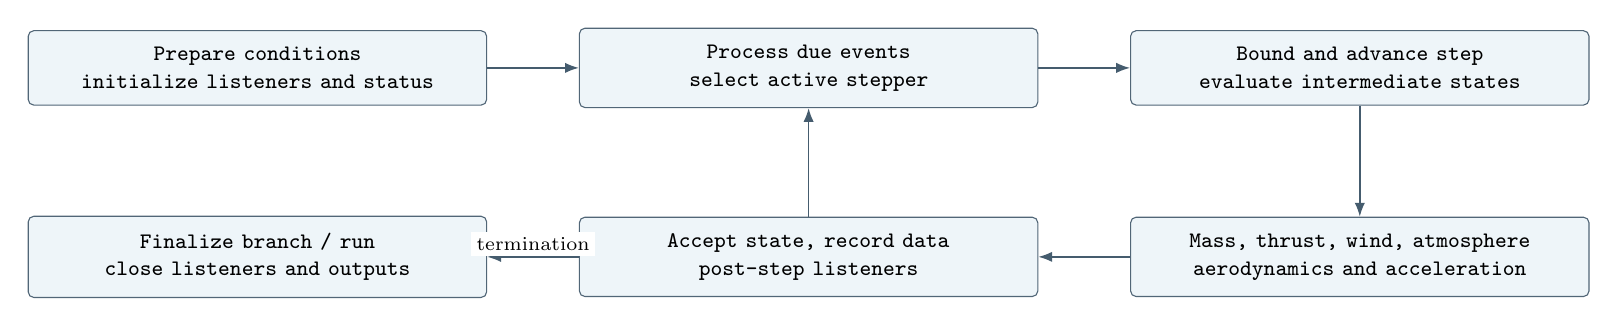
\begin{tikzpicture}
\simple{prepare}{0,0}{Prepare conditions\\initialize listeners and status}{5.4cm}
\simple{events}{7,0}{Process due events\\select active stepper}{5.4cm}
\simple{step}{14,0}{Bound and advance step\\evaluate intermediate states}{5.4cm}
\simple{end}{0,-2.4}{Finalize branch / run\\close listeners and outputs}{5.4cm}
\simple{record}{7,-2.4}{Accept state, record data\\post-step listeners}{5.4cm}
\simple{models}{14,-2.4}{Mass, thrust, wind, atmosphere\\aerodynamics and acceleration}{5.4cm}
\draw[use] (prepare) -- (events);
\draw[use] (events) -- (step);
\draw[use] (step) -- (models);
\draw[use] (models) -- (record);
\draw[use] (record) -- (events);
\draw[use] (record) -- node[flowlabel,above]{termination} (end);
\end{tikzpicture}}

\section{What the flight stepper computes}
\class{RK4SimulationStepper} and \class{RK6SimulationStepper} separately implement their Runge--Kutta schemes. They share \class{AbstractSimulationStepper} services, but RK6 is not a subclass of RK4. Both evaluate multiple provisional states within one accepted time interval. The calculations include:
\begin{enumerate}
\item Query atmospheric and wind conditions and transform relative airflow into the body frame.
\item Calculate aerodynamic coefficients, structure/motor mass, current thrust, and gravity.
\item Convert coefficients to dimensional forces and moments; shift pitch/yaw moments to the current CG.
\item Divide force by mass and the supported moment components by effective inertias; rotate acceleration to the world frame and apply gravity/Coriolis terms.
\item Integrate translation, rotation rate, and quaternion orientation; update world position from local displacement.
\end{enumerate}

Conceptually the translation follows \(\dot{\boldsymbol r}=\boldsymbol v\) and \(\dot{\boldsymbol v}=\boldsymbol a\). The angular implementation uses the calculated pitch/yaw/roll moments and longitudinal/rotational inertia values. It should not be described as a general full-tensor, flexible, or coupled multibody dynamics solution. The source's supported moment and frame conventions are the actual contract.

Before liftoff, the code prevents downward motion through the pad. While the rocket remains on the launch rod, acceleration is projected onto the rod direction and angular acceleration is constrained. The MIT initial-roll-rate option prescribes longitudinal spin, including on a tilted rod; it is not generated by a modeled rail friction or spin-up mechanism.

\section{Timestep selection and fork-specific behavior}
The flight steppers contain limits for configured step size, event distance, angular change, rate change, launch-rod travel, and growth relative to the previous step. However, the non-FC branch retains legacy MIT static timestep controls from \class{MidControlStepLauncher}; it can replace the initially selected step with \code{theTimeStep}. This must be considered when interpreting the ordinary simulation-options timestep field or comparing the fork to vanilla behavior.

With an active FC, the engine/steppers instead honor the FC deadline cap and maximum physics step. The FC path avoids floors or overrides that would skip an imminent virtual deadline. Its default cap is 2.5 ms. The ensemble listener supplies an additional step cap based on the thrust-noise interval. Reducing a step improves temporal resolution but does not repair an incorrect physical submodel or an inconsistent frame transform.

\section{Listener lifecycle and accepted measurements}
\class{SimulationListenerHelper} dispatches lifecycle and calculation hooks. Pre-calculation hooks may supply replacements; post-calculation hooks may inspect or modify values according to their contracts. Step and event callbacks have different semantics from intermediate aerodynamic/acceleration callbacks.

Stateful onboard logic must not execute once for every provisional Runge--Kutta evaluation. The FC listener captures a coherent first-stage acceleration/status acquisition and publishes it only after the interval is accepted. It advances due work at explicit virtual deadlines. This preserves the distinction between a physical derivative evaluation and one firmware loop iteration. The \code{preStep} callback prepares an interval; \code{limitStep} is called by the engine/stepper to enforce its boundary.

\section{Descent, termination, and result publication}
Recovery deployment switches to \class{BasicLandingStepper}; tumbling uses \class{BasicTumbleStepper}; grounded behavior has its own stepper. Landing/tumble derive from \class{AbstractEulerStepper}, which updates translation with its specialized drag model and event-aware limits. Those paths do not integrate a new attitude history, so recorded orientation is held rather than inventing a canopy-hanging or tumbling animation.

The engine records warnings and aborts separately from ordinary samples. Maximum duration, ground impact, explicit aborts, exceptions, and cancellation can end work through different paths. Consumers should inspect the recorded events/warnings and worker outcome rather than infer success merely from the existence of a \class{FlightData} object. Listener shutdown closes per-run resources; the FC removes live execution from auxiliary optimum-coast calculations to avoid advancing its clock a second time.

\sourceline{\source{core/src/main/java/info/openrocket/core/document/Simulation.java}{Simulation.simulateInternal}; \source{core/src/main/java/info/openrocket/core/simulation/ModifiedEventSimulationEngine.java}{ModifiedEventSimulationEngine}; \source{core/src/main/java/info/openrocket/core/simulation/SimulationStatus.java}{SimulationStatus}; \source{core/src/main/java/info/openrocket/core/simulation/RK4SimulationStepper.java}{RK4SimulationStepper}; \source{core/src/main/java/info/openrocket/core/simulation/RK6SimulationStepper.java}{RK6SimulationStepper}; \source{core/src/main/java/info/openrocket/core/simulation/AbstractEulerStepper.java}{AbstractEulerStepper}.}

\section{Ordinary launch, powered flight, and coast}
Run initialization selects active stages and motor installations, builds the initial event queue, establishes pad position and orientation, and initializes listeners. Orientation incorporates launch-rod inclination and bearing; the status also selects an initial roll orientation relative to the flight-condition convention. The initial-spin setting is a separate MIT addition.

The launch event can activate configured motors after their ignition delays. Ignition begins a motor's local clock; burnout ends thrust; ejection follows the selected delay where applicable. Liftoff and rod clearance are physical milestones distinct from ignition. Before liftoff the vehicle cannot translate downward through the pad, and while constrained by the rod the solver projects acceleration onto the guide direction.

\class{SimulationStatus} computes effective guide travel from configured rod length and the aftmost modeled launch-lug position. With no lugs it assumes a full-length tower launcher. The inspected loop specifically checks \class{LaunchLug}; the presence of a \class{RailButton} is not equivalent to that lug-length correction. The rod model constrains motion but does not simulate rail bending, button contact friction, or mechanical release loads.

After burnout, aerodynamic forces, gravity, wind, and changing configuration continue to govern coast. The engine detects apogee and altitude transitions, schedules recovery/staging rules, and records warnings and milestones. If deployment occurs before the natural coast apex, an auxiliary optimum-coast calculation can estimate the altitude and time that would have been reached without that deployment. This supports optimum-delay reporting; it is not a second observed flight history.

\section{What a numerical step means}
A Runge--Kutta step forms provisional positions, velocities, orientations, and rates at prescribed substep times, evaluates the derivatives there, and combines them into the accepted endpoint. The quaternion represents orientation without Euler-angle singularities, but it must remain normalized and used with the correct transform direction. The world angular-rate vector and body aerodynamic rates are related by rotation; they are not interchangeable arrays of three numbers.

The stepper records the force/mass/condition quantities associated with its accepted data point and supplies calculated events to the engine. Event-aware limits prevent stepping blindly beyond a known ignition, ejection, or other scheduled boundary. The retained RK4 and MIT RK6 implementations have different stage formulas and can have different limiting behavior; their names alone do not establish a formal adaptive local-error tolerance. The ordinary maximum timestep and angular-step settings express the actual available controls.

Exceptions separate cancellation, calculation failure, listener termination, and other run failures. System listeners such as ground-hit or recovery-stop listeners can serve special computations with different stopping rules. A headless caller must still interpret warnings/events and close run resources, rather than merely checking that the method returned an object.

\section{Tumble and grounded modes}
The tumble stepper is a translational empirical descent model. It combines symmetric-body projected area with fin planform area and fin-count efficiency factors. The coefficients in \class{BasicTumbleStepper} are 0.56 for the body contribution and 1.42 for the effective fin contribution, normalized to rocket reference area. The fin-count table approximates exposure during tumble. This is not rotational integration of a tumbling rigid body.

Landing and tumble use \class{AbstractEulerStepper}, while \class{GroundStepper} handles grounded continuation. The engine can change the stepper while retaining the branch's identity and event history. A held quaternion after deployment/tumble reflects this numerical model, not measured canopy alignment. These mode changes must be respected by plots, physical sensors, and extensions that continue through descent.

\sourceline{\source{core/src/main/java/info/openrocket/core/simulation/SimulationStatus.java}{initialization and guide length}; \source{core/src/main/java/info/openrocket/core/simulation/BasicEventSimulationEngine.java}{inherited event lifecycle}; \source{core/src/main/java/info/openrocket/core/simulation/BasicTumbleStepper.java}{BasicTumbleStepper}; \source{core/src/main/java/info/openrocket/core/simulation/GroundStepper.java}{GroundStepper}; \source{core/src/main/java/info/openrocket/core/simulation/listeners/system/OptimumCoastListener.java}{OptimumCoastListener}.}


\chapter{Parachutes, recovery systems, and stage separation}\label{ch:recovery}
Recovery spans three layers: a component describes the device; a deployment rule or FC command decides when deployment is requested; the engine changes the actual flight state. A logical firing pulse, queued event, accepted deployment, and changed descent drag are distinct observations.

\section{Device geometry and mass}
\class{RecoveryDevice} is the common abstraction for parachutes and streamers. It supplies projected area, drag coefficient behavior, material-derived mass, and per-flight deployment configuration. \class{Parachute} derives canopy area from diameter and includes line mass from line count, length, and line material. \class{Streamer} derives area from its dimensions. Packed position and dimensions support placement and mass modeling inside the rocket.

The canopy shown during flight playback is a visual indicator of actual deployment. It is not the mesh used to calculate drag. Likewise, a shock cord component contributes modeled properties but does not create a dynamic tether constraint, elasticity, or opening-shock calculation between separated bodies.

\section{Ordinary OpenRocket deployment rules}
\class{DeploymentConfiguration} is indexed by flight configuration. Its event choices include launch, same-stage motor ejection, apogee, a descending altitude crossing, lower-stage separation, and never. A configured delay is added after the activating event. The engine checks active stages and dispatches the resulting \class{FlightEvent.Type.RECOVERY_DEVICE_DEPLOYMENT} through the listener system.

Altitude deployment detects a crossing using the previous/current altitude pair, not a statement that the rocket is simply below a threshold at any time. Ejection matching is stage-aware. Stage-separation-triggered recovery uses the relevant neighboring-stage relationship. These details prevent rules from being interpreted as interchangeable generic timers.

\section{Inherited parachute and streamer force laws}
A parachute's deployed area is $A=\pi d^2/4$ for the configured canopy diameter. Its baseline drag coefficient is 0.8 unless a preset or explicit setting supplies another value. The current component method returns its coefficient without a Mach-dependent canopy model. Structural mass is canopy area times surface density, plus line count times line length times line density. Canopy porosity, spill holes, inflation history, and suspension-line geometry are not separately resolved in this coefficient.

A streamer's area is strip length times width, and its material mass uses surface density. With automatic CD, the implementation estimates
\begin{equation}
C_{D,\rm streamer}=\min\left[0.4,\ 0.034\frac{\sigma+0.025}{0.105}\frac{\ell+1}{\ell}\right],
\end{equation}
using the source's SI-valued strip length $\ell$ and surface density $\sigma$. The numerical constants belong to this empirical relation. A manual coefficient bypasses the automatic estimate through \class{RecoveryDevice}'s coefficient-selection path. Width still changes drag through area even though it does not appear explicitly in this CD formula.

Once deployed, each device contributes $C_D A$ to the landing stepper. Increasing canopy diameter therefore changes both drag area and material mass; entering an explicit mass override can separate those effects. Multiple deployed devices add their effective drag areas. There is no canopy-shadowing or entanglement calculation between a drogue and main.

For intuition only, balancing weight against drag in still air at fixed density gives $V_t\approx\sqrt{2mg/(\rho\sum C_DA)}$. The simulation integrates acceleration instead of instantly assigning this terminal speed, and wind and altitude-dependent density change the trajectory. This estimate is a useful interpretation of the implemented area sum, not an additional algorithm in the code.

\section{Ordinary staging and two-device recovery}
Independent deployment configurations let a drogue activate at apogee and a main activate on a descending-altitude crossing with its own delay. They share the stage's evolving status but retain separate device identity. A never-deploy rule leaves a device as packed mass unless another authorized path deploys it. The configured deployment threshold is evaluated through altitude events, so it should not be confused with geographic MSL altitude or the FC's zeroed barometric height.

Stage separation has its own event selector: launch; current-stage ignition, burnout, or ejection; upper-stage ignition; ascending altitude; apogee; descending altitude; or never. A separate delay applies after activation. A separation trigger does not itself prescribe a parachute opening, and a motor ejection event does not necessarily separate a stage unless the stage rule says so. After a split, active-component filtering determines the motors and recovery devices available to each branch.

\sourceline{\source{core/src/main/java/info/openrocket/core/rocketcomponent/Parachute.java}{Parachute}; \source{core/src/main/java/info/openrocket/core/rocketcomponent/Streamer.java}{Streamer}; \source{core/src/main/java/info/openrocket/core/rocketcomponent/RecoveryDevice.java}{RecoveryDevice coefficient selection}; \source{core/src/main/java/info/openrocket/core/rocketcomponent/StageSeparationConfiguration.java}{StageSeparationConfiguration}.}


\section{Exclusive FC recovery mode}
When FC simulation is enabled, both event engines suppress ordinary automatic deployment scheduling. Only events owned by the FC recovery bridge are accepted as FC-authorized recovery events. Saved ordinary deployment settings remain in the rocket and resume when FC simulation is disabled. There is no automatic fallback for an unassigned parachute.

The simulation's FC configuration maps shared logical channels 0--5 to recovery-device UUIDs and per-device delays. One channel can command several devices; several channels can provide redundant commands for one device. The bridge schedules only the first accepted request for each device, so repeated pulses cannot restart its delay.

\begin{equation}
 t_{\mathrm{deploy}}=t_{\mathrm{accepted\ command,boot}}-t_{\mathrm{warmup}}+\Delta t_{\mathrm{device}}.
\end{equation}
The command timestamp is the completion time of the relevant FC/Java action, retained at microsecond precision. A pyro pulse's duration is not a deployment delay. Warm-up commands before physical time zero are discarded physically, and commands after landing cannot deploy a device. Recovery timing does not wait for PWM or telemetry reception.

\section{Actual deployment and descent}
When handling a deployment event, the engine checks that the stage is active. It retains the existing under-thrust abort behavior, launch-rod warning, and high-speed-deployment warning. Listeners can veto events or deployment. A successful deployment adds the device to the status's deployed set, records the event, acknowledges FC provenance when applicable, and switches to the landing stepper if still airborne.

The landing stepper sums effective drag areas for deployed instances:
\begin{equation}
 C_{D,\mathrm{landing}}=\sum_{j\in\mathrm{deployed}}
 n_j C_{D,j}\frac{A_j}{S_{\mathrm{ref}}}.
\end{equation}
It then uses the descent integration path with atmospheric conditions, mass, gravity, and wind. The sum is the recovery-stepper drag model; it should not be assumed to be a complete addition of every ascent-airframe aerodynamic term. Ensemble drag scaling is explicitly applied to this descent coefficient too.

Drogue deployment does not end the FC. The same per-flight runtime continues while the landing stepper advances time, allowing a later main event. The bridge records actual device name/ID, origin channel, due time, deployment time, and lateness. Those events survive ORK storage and supported log import and drive the 3D canopy display.

\section{Stage separation and branch identity}
An ordinary staged simulation can split into multiple branches. At separation, the engine copies status, creates a booster result branch, clears the appropriate active-stage subsets in booster and continuing configurations, removes unattached pending events, and queues the detached branch for simulation. Each branch uses its remaining hardware and motor/recovery state.

The FC path currently requires exactly one active stage at startup and does not support arbitrary multistage FC ownership or mid-flight checkpoint boot. The general engine's ability to branch should not be mistaken for support for an independent FC on every resulting stage.

\section{Model boundaries and debugging order}
Opening inflation, reefing/cutaway, tether tension, separation impulses, electrical firing energy, and detailed canopy attitude dynamics are outside the current recovery model. Continuity/status bits are logical firmware observations, not evidence of a successful physical canopy deployment.

To investigate a missed deployment, follow the chain in order: logical output present; arming/accepted command; channel mapping; device active; warm-up/landing eligibility; scheduled event; listener acceptance; engine abort conditions; actual deployment record; descent drag. This identifies whether the problem is firmware decision logic, mapping, event authority, or physical integration without conflating those layers.

\sourceline{\source{core/src/main/java/info/openrocket/core/rocketcomponent/RecoveryDevice.java}{RecoveryDevice}; \source{core/src/main/java/info/openrocket/core/rocketcomponent/Parachute.java}{Parachute}; \source{core/src/main/java/info/openrocket/core/rocketcomponent/DeploymentConfiguration.java}{DeploymentConfiguration}; \source{core/src/main/java/info/openrocket/core/simulation/BasicLandingStepper.java}{BasicLandingStepper}; \source{core/src/main/java/info/openrocket/core/simulation/flightcomputer/FlightComputerRecoveryBridge.java}{FlightComputerRecoveryBridge}; \source{core/src/main/java/info/openrocket/core/simulation/ModifiedEventSimulationEngine.java}{ModifiedEventSimulationEngine}.}

\chapter{Flight-computer simulation and control}\label{ch:fc}
This chapter carries forward the complete FC architecture report of 11 October 2026, including its nine native TikZ diagrams and firmware class index. The unchanged original TeX and PDF are preserved under \code{reference/}. Integration clarifications below describe the source snapshot used by this larger guide. Historical verification numbers remain dated evidence from that report; they are not results of a new application test run.

\section{Scope and namespace migration}
The former \code{edu.mit.rocket_team.zephyrus} root has become
\code{edu.mit.rocket_team}. Subpackages such as \code{FC}, \code{instrument},
\code{control} and \code{telemetry} remain. The change updates source paths,
package declarations, imports, module exports, tests and live documentation references.

\begin{lstlisting}[language=Java]
// Previous: edu.mit.rocket_team.zephyrus.FC.RTFC
import edu.mit.rocket_team.FC.RTFC;
\end{lstlisting}

There is no compatibility package at the old namespace. External source that
imports these firmware classes must update its imports, and compiled clients
must be rebuilt. Custom boards using the supported API
\code{info.openrocket.core.simulation.flightcomputer.JavaBoardProgram}
do not require an import change.

Firmware model identifiers, \code{.fc} schema versions, telemetry byte layouts,
existing log prefixes and the extension class \class{ZephyrusFlightComputer}
retain their identities. Saved design and simulation-extension references can
therefore continue to load. Historical benchmark logs retain their meaning as
records of the builds that produced them.

\subsection{Readability and documentation coverage}
The source manifest covers the translated firmware and Java files introduced
for the FC designer, controller blocks, physical actuator and recovery bridges,
sensor models, telemetry replay, ensembles, motor batches, 3D plotting,
update/memory helpers, tests and standalone verification tools.

Methods use consistent four-space formatting with blank-line separation.
Every explicit method and constructor in that manifest has a Javadoc description,
including private helpers and anonymous-class callbacks. Compiler-generated
record accessors and implicit constructors are not explicit source declarations.

Selected pre-existing OpenRocket integration classes are included in the
browsable reference for context. They are outside the newly documented-method
coverage requirement; malformed comments and stale links encountered during
Javadoc generation were repaired. The application runtime did not acquire a
new documentation dependency.

\subsection{Behavior preservation and reading the diagrams}
The parser comparison found identical executable token streams in all 150
original scoped files after ignoring comments/formatting and normalizing the
namespace. This comparison concerns this refactor; previously implemented
controller and recovery features retain their own functional changes.

Class diagrams show selected operations rather than reproducing the entire
API. A hollow triangle points to a superclass or interface; a filled diamond
marks an owning runtime relationship; ordinary arrows denote use or data flow.
Sequence diagrams describe virtual ordering, not desktop wall-clock latency.
The full method reference is generated in \code{doc/improvements/javadoc/}.

\clearpage
\section{Connection to the OpenRocket engine}
In this fork, \class{Simulation.simulate()} constructs \class{ModifiedEventSimulationEngine}; its flight stepper defaults to RK6 through \code{NewControlStepListener.useRK6}. Both \class{BasicEventSimulationEngine}
and \class{ModifiedEventSimulationEngine} use the existing listener lifecycle
and advance a physical stepper. \class{SimulationStatus} carries physical state,
conditions, active components and the result branch. The FC extension freezes
and validates its external design, checks custom Java approval and installs
one \class{FlightControllerSimulatorListener}.

\diagram{fig:engine}{Engine integration. The existing extension and listener connect the renamed runtime to the physical simulation.}{%
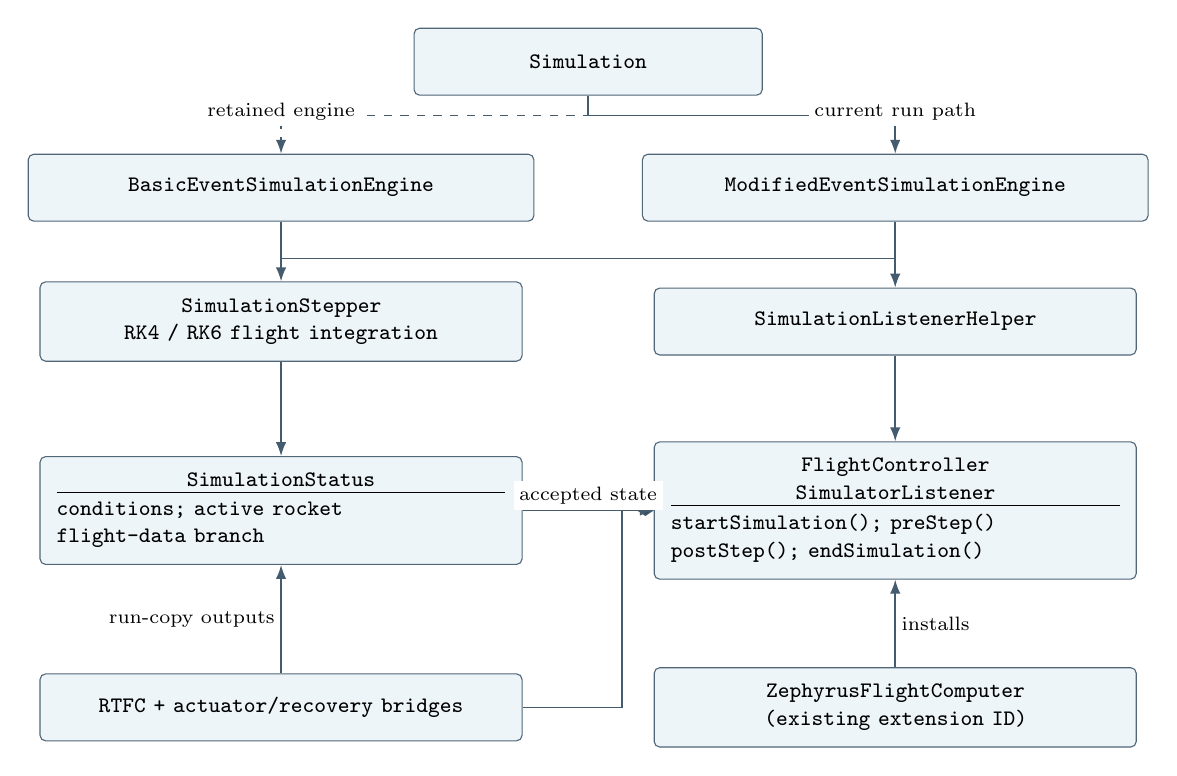
\begin{tikzpicture}
\simple{sim}{7.7,0}{Simulation}{4cm}
\simple{basic}{3.8,-1.6}{BasicEventSimulationEngine}{6cm}
\simple{modified}{11.6,-1.6}{ModifiedEventSimulationEngine}{6cm}
\simple{step}{3.8,-3.3}{SimulationStepper\\RK4 / RK6 flight integration}{5.7cm}
\simple{helper}{11.6,-3.3}{SimulationListenerHelper}{5.7cm}
\uml{status}{3.8,-5.7}{SimulationStatus}{conditions; active rocket\\flight-data branch}{5.7cm}
\uml{listener}{11.6,-5.7}{FlightController\\SimulatorListener}{startSimulation(); preStep()\\postStep(); endSimulation()}{5.7cm}
\simple{ext}{11.6,-8.2}{ZephyrusFlightComputer\\(existing extension ID)}{5.7cm}
\simple{fc}{3.8,-8.2}{RTFC + actuator/recovery bridges}{5.7cm}
\draw[use,dashed] (sim.south) -- ++(0,-0.25) -| node[flowlabel,pos=.65,above]{retained engine} (basic.north);
\draw[use] (sim.south) -- ++(0,-0.25) -| node[flowlabel,pos=.65,above]{current run path} (modified.north);
\draw[use] (basic.south) -- (3.8,-2.5) -- (step.north);
\draw[use] (modified.south) -- (11.6,-2.5) -- (helper.north);
\draw[draw=ink!80,line width=.55pt] (3.8,-2.5) -- (11.6,-2.5);
\draw[use] (step) -- (status);
\draw[use] (helper) -- (listener);
\draw[use] (ext) -- node[flowlabel,right]{installs} (listener);
\draw[own] (listener.west) -- ++(-0.4,0) |- (fc.east);
\draw[use] (status.east) -- node[flowlabel,above]{accepted state} (listener.west);
\draw[use] (fc) -- node[flowlabel,left]{run-copy outputs} (status);
\end{tikzpicture}}

The listener creates a fresh \class{RTFC}, per-run context, telemetry outputs
and physical bindings. Servo and cant changes apply to the simulation's rocket
copy, preserving the user's design. \code{preStep} prepares the interval and applies latched outputs; the engine and steppers call \code{limitStep} to cap the next physical step at a virtual deadline. Coherent accepted acceleration/status samples feed
acquisition; intermediate or future states are not replayed as earlier sensor
measurements. \code{postStep} advances due work and synchronizes FC/physical
result channels. Run shutdown closes outputs and pending recovery work.
The separate \class{AirbrakesControllerListener} is not part of this FC path.

\clearpage
\section{Per-run runtime composition}
\class{RTFC} owns the translated instruments and firmware controllers.
Design-defined state graphs, controller blocks and Java boards extend that
runtime. \class{RTFC.Inputs} carries engineering-unit acquisitions and their
timestamps. \class{RTFC.Output} is the PWM-latched snapshot, including legacy
channels, named servo maps and per-controller outputs.

\diagram{fig:runtime}{Run-local state and the boundaries between acquisitions, task execution and latched outputs.}{%
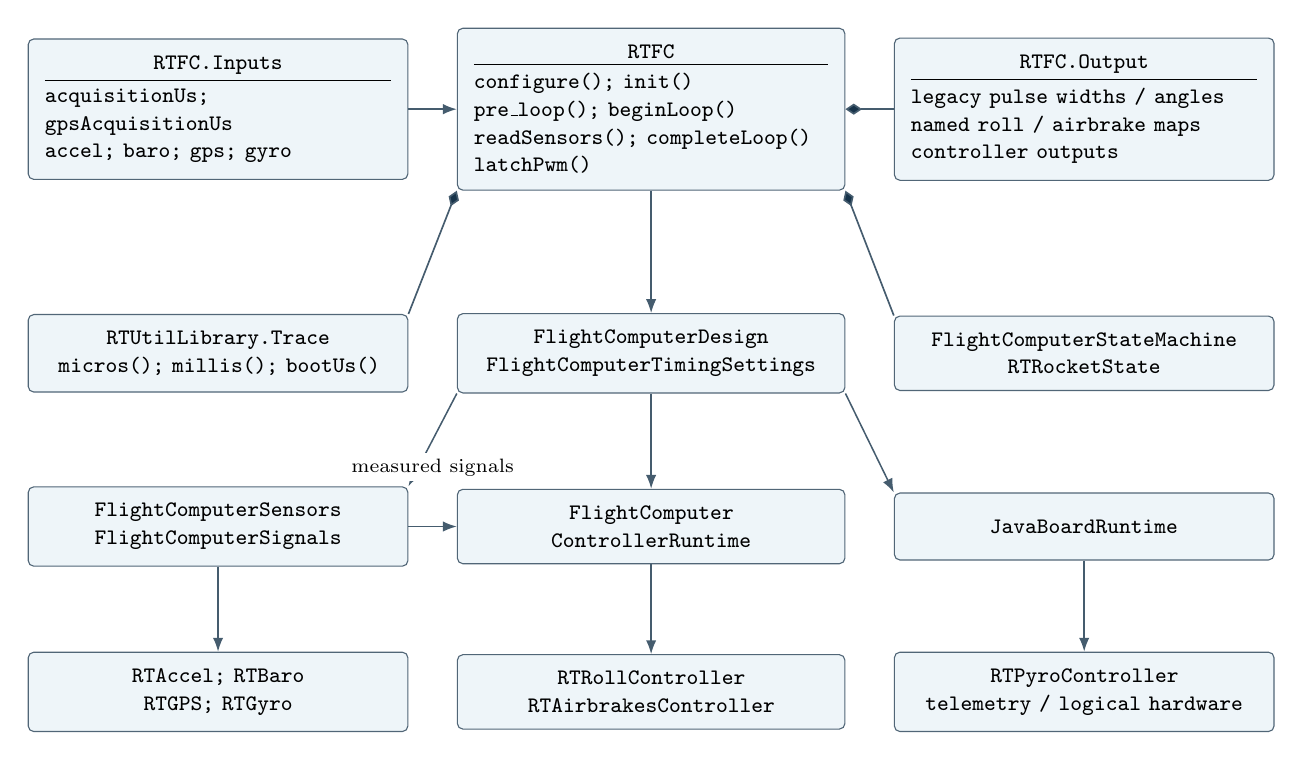
\begin{tikzpicture}
\uml{inputs}{2.5,0}{RTFC.Inputs}{acquisitionUs; gpsAcquisitionUs\\accel; baro; gps; gyro}{4.4cm}
\uml{fc}{8,0}{RTFC}{configure(); init()\\pre\_loop(); beginLoop()\\readSensors(); completeLoop()\\latchPwm()}{4.5cm}
\uml{out}{13.5,0}{RTFC.Output}{legacy pulse widths / angles\\named roll / airbrake maps\\controller outputs}{4.4cm}
\simple{clock}{2.5,-3.1}{RTUtilLibrary.Trace\\micros(); millis(); bootUs()}{4.4cm}
\simple{design}{8,-3.1}{FlightComputerDesign\\FlightComputerTimingSettings}{4.5cm}
\simple{state}{13.5,-3.1}{FlightComputerStateMachine\\RTRocketState}{4.4cm}
\simple{sensors}{2.5,-5.3}{FlightComputerSensors\\FlightComputerSignals}{4.4cm}
\simple{blocks}{8,-5.3}{FlightComputer\\ControllerRuntime}{4.5cm}
\simple{boards}{13.5,-5.3}{JavaBoardRuntime}{4.4cm}
\simple{inst}{2.5,-7.4}{RTAccel; RTBaro\\RTGPS; RTGyro}{4.4cm}
\simple{control}{8,-7.4}{RTRollController\\RTAirbrakesController}{4.5cm}
\simple{services}{13.5,-7.4}{RTPyroController\\telemetry / logical hardware}{4.4cm}
\draw[use] (inputs) -- (fc);
\draw[own] (fc) -- (out);
\draw[own] (fc.south west) -- (clock.north east);
\draw[use] (fc) -- (design);
\draw[own] (fc.south east) -- (state.north west);
\draw[use] (design.south west) -- (sensors.north east);
\draw[use] (design) -- (blocks);
\draw[use] (design.south east) -- (boards.north west);
\draw[use] (sensors) -- (inst);
\draw[use] (blocks) -- (control);
\draw[use] (boards) -- (services);
\draw[use] (sensors.east) -- node[flowlabel,above=16pt]{measured signals} (blocks.west);
\end{tikzpicture}}

The trace is a virtual boot clock and action sink shared by the run's devices.
Sensor histories, task instances, controller state and channel caches belong
to the run. A new simulation receives fresh instances. Physical comparison
curves are recorded separately from the measurements used by controllers.
Logical commands and PWM-latched physical commands are separate states.

\clearpage
\section{Timing contracts}
Boot timestamps are integer microseconds. Physical simulation time zero
follows \(1{,}000{,}000\us\) of virtual warm-up. The preflight command is queued
at \(500{,}000\us\) during warm-up. Firmware \code{micros()} and \code{millis()}
retain unsigned 32-bit wrap; the trace additionally stores unwrapped boot time.
For clocks in the same units, the firmware elapsed-time operation is
\begin{equation}
 \Delta t_{32}=(t_{\mathrm{now}}-t_{\mathrm{then}})\bmod 2^{32}.
\end{equation}

\begin{table}[htbp]\centering\small
\begin{tabularx}{\linewidth}{@{}L{3.1cm}Y@{}}\toprule
Boundary & Implemented contract\\\midrule
FC loop & Nominal 10,000\us\ period, with modeled sensor-read cost, extra work and seeded execution jitter. Loop phases cannot overlap.\\
Held acquisition & Input acquisition and availability times are distinct. A loop uses its held acquisition; GPS retains the original fix timestamp.\\
Independent tasks & Java boards and controller blocks freeze inputs at start, publish at completion and follow independent periods and execution costs.\\
PWM & Commands latch every 20,000\us\ with configurable phase. A task completing exactly on an interrupt boundary misses that latch.\\
State epochs & State changes invalidate work begun in an earlier state; explicit controller-close actions invalidate pending block work.\\
Recovery & Accepted commands retain completion time in microseconds. Physical deployment deadlines do not wait for servo PWM or radio delivery.\\
\bottomrule\end{tabularx}
\caption{Virtual contracts enforced by the existing listener scheduler.}
\end{table}

The firmware's nominal wait is millisecond-quantized. For loop start \(s_n\)
and completion \(c_n\), both in boot microseconds,
\begin{equation}
 s_{n+1}=\max\!\left(c_n,\;1000\left(\left\lfloor\frac{s_n}{1000}\right\rfloor+10\right)\right).
\end{equation}
A custom board or controller block instead uses its own configured period
\(P\):
\begin{equation}
 s_{n+1}=\max(s_n+P,\;c_n).
\end{equation}
An overrun delays the next invocation; it does not create overlapping calls
or a catch-up burst. A faster task does not create fresher measurements.

These are virtual-time contracts. The desktop's elapsed execution time is
not the modeled processor time. Execution costs remain supplied approximations;
board grouping does not simulate shared CPU arbitration or communications
contention between physical boards.

\clearpage
\subsection{Dispatch ordering and the PWM completion tie}
At a coincident boundary, PWM latching precedes FC completion, then controller
and Java-board work. Figure~\ref{fig:scheduler} shows the relevant ordering;
GPS availability and other due services remain part of the same dispatcher.

\diagram{fig:scheduler}{Virtual scheduling: a command completed at the PWM instant is available only after that instant's latch.}{%
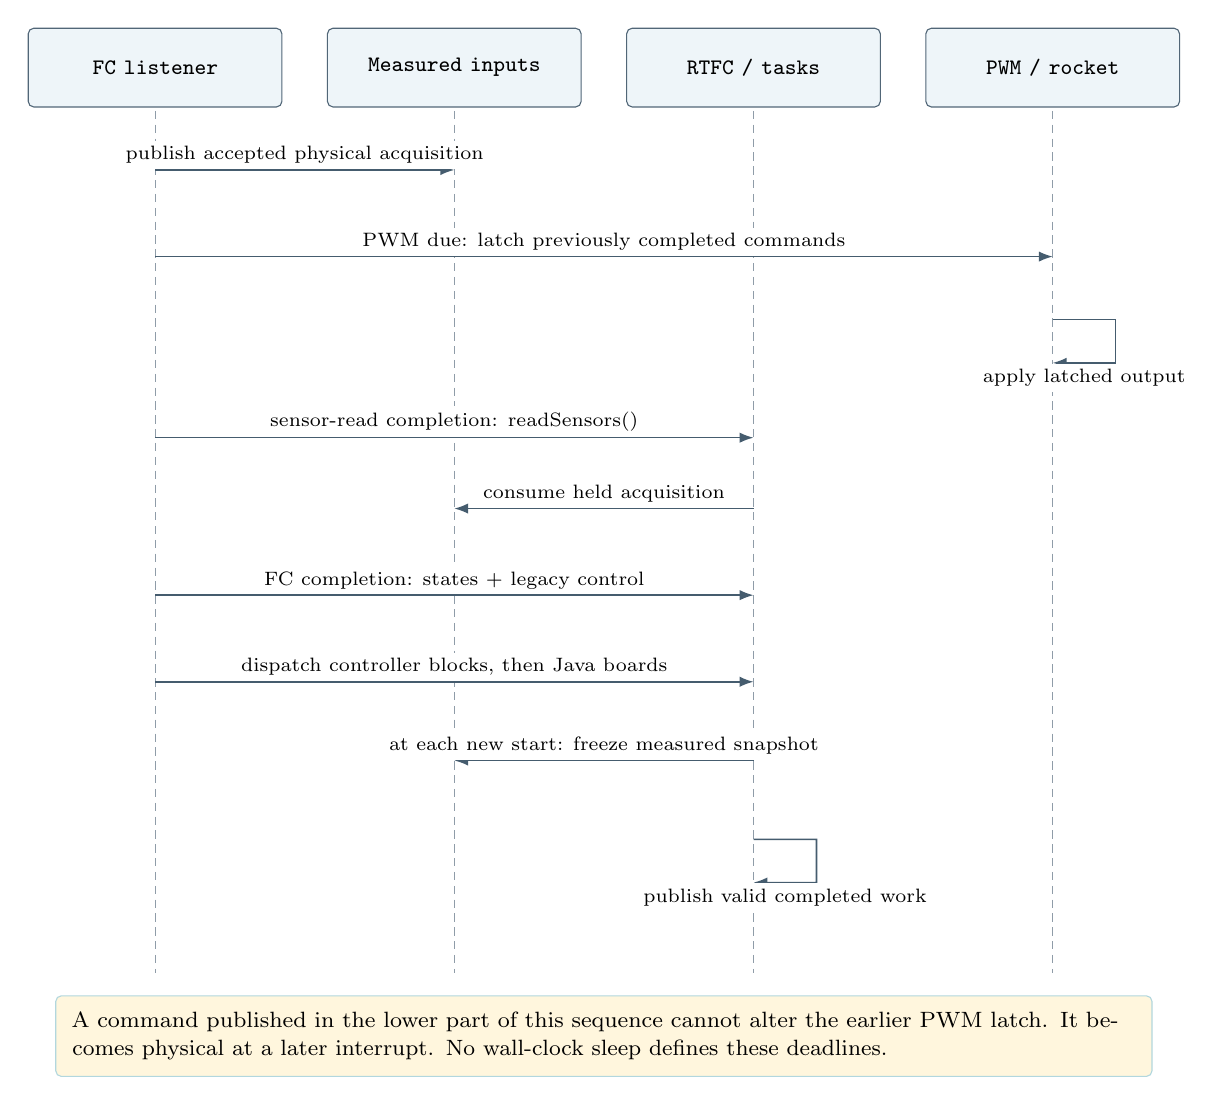
\begin{tikzpicture}
\node[participant,text width=2.8cm] (l) at (1.5,0) {\ttfamily FC listener};
\node[participant,text width=2.8cm] (s) at (5.3,0) {\ttfamily Measured inputs};
\node[participant,text width=2.8cm] (f) at (9.1,0) {\ttfamily RTFC / tasks};
\node[participant,text width=2.8cm] (p) at (12.9,0) {\ttfamily PWM / rocket};
\foreach \x in {1.5,5.3,9.1,12.9} \draw[lifeline] (\x,-0.55) -- (\x,-11.5);
\draw[use] (1.5,-1.3) -- node[flowlabel,above]{publish accepted physical acquisition} (5.3,-1.3);
\draw[use] (1.5,-2.4) -- node[flowlabel,above]{PWM due: latch previously completed commands} (12.9,-2.4);
\draw[use] (12.9,-3.2) -- ++(0.8,0) -- ++(0,-0.55) -- node[flowlabel,below]{apply latched output} (12.9,-3.75);
\draw[use] (1.5,-4.7) -- node[flowlabel,above]{sensor-read completion: readSensors()} (9.1,-4.7);
\draw[use] (9.1,-5.6) -- node[flowlabel,above]{consume held acquisition} (5.3,-5.6);
\draw[use] (1.5,-6.7) -- node[flowlabel,above]{FC completion: states + legacy control} (9.1,-6.7);
\draw[use] (1.5,-7.8) -- node[flowlabel,above]{dispatch controller blocks, then Java boards} (9.1,-7.8);
\draw[use] (9.1,-8.8) -- node[flowlabel,above]{at each new start: freeze measured snapshot} (5.3,-8.8);
\draw[use] (9.1,-9.8) -- ++(0.8,0) -- ++(0,-0.55) -- node[flowlabel,below]{publish valid completed work} (9.1,-10.35);
\node[note,text width=13.5cm] at (7.2,-12.3) {A command published in the lower part of this sequence cannot alter the earlier PWM latch. It becomes physical at a later interrupt. No wall-clock sleep defines these deadlines.};
\end{tikzpicture}}

Controller-block completion must also belong to the current state epoch. Block work invalidated
by a state change cannot publish stale control output. Java boards retain their own start-time state snapshots and independent schedules; they do not share the block epoch-cancellation mechanism. The engine's next
physical step is capped at the next pending virtual deadline so the scheduler
does not recreate missed loop ticks using future physical samples.

\clearpage
\section{Measurements and coordinate conventions}
\class{FlightComputerSensors} applies configured mounting rotation, bias,
acquisition cadence and seeded Gaussian noise to accepted simulator inputs.
\class{FlightComputerSignals} publishes stable source IDs, channel descriptors,
validity and acquisition/availability times. Primary sensors retain firmware
filtering and integration; additional sensors keep independent histories.

\diagram{fig:sensors}{Instrument adapters and injected payloads. Hollow triangles identify the two shared base classes.}{%
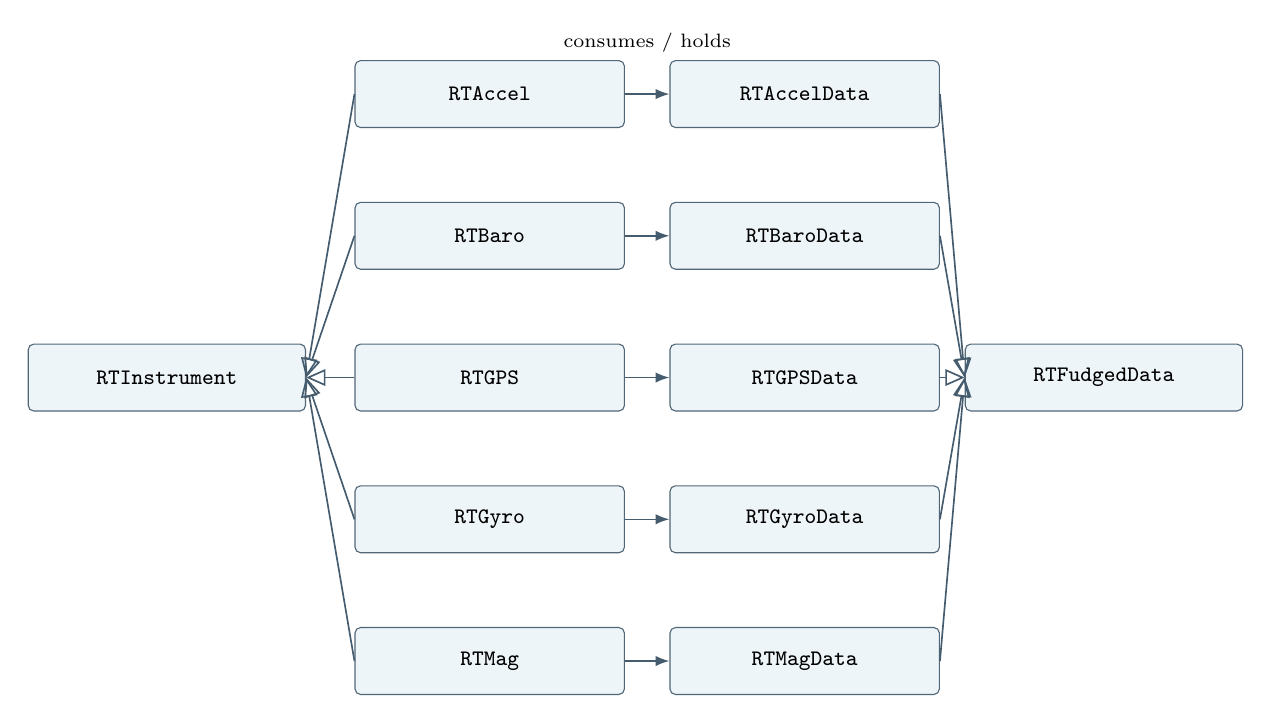
\begin{tikzpicture}
\simple{base}{1.9,-3.6}{RTInstrument}{3.1cm}
\simple{payload}{13.8,-3.6}{RTFudgedData}{3.1cm}
\foreach \name/\data/\yy in {RTAccel/RTAccelData/0,RTBaro/RTBaroData/-1.8,RTGPS/RTGPSData/-3.6,RTGyro/RTGyroData/-5.4,RTMag/RTMagData/-7.2} {
 \simple{\name}{6.0,\yy}{\name}{3cm}
 \simple{\data}{10.0,\yy}{\data}{3cm}
 \draw[inherit] (\name.west) -- (base.east);
 \draw[use] (\name.east) -- (\data.west);
 \draw[inherit] (\data.east) -- (payload.west);
}
\node[flowlabel] at (8,0.65) {consumes / holds};
\end{tikzpicture}}

\begin{table}[htbp]\centering\small
\begin{tabularx}{\linewidth}{@{}L{2.4cm}Y@{}}\toprule
Quantity & Interface convention\\\midrule
Acceleration & Specific force in m/s\(^2\); FC sensor X is OpenRocket body Z. The legacy velocity estimate integrates sensor X minus gravity, rather than ground-speed magnitude or airspeed.\\
Angular rate & Sensor rates in degrees/s. Roll integrates negative sensor X; pitch/yaw use the corresponding held rates.\\
Barometer & Pressure in hPa, temperature in Celsius and height in metres. Pressure altitude passes through the moving average and zero reference.\\
GPS & Input coordinates are decimal degrees and altitude is MSL metres; quantization is \(10^{-7}\) degrees and millimetres. The adapter's \code{getHeight()} and \code{getAltitude()} return zero-relative height.\\
Raw counts & Pressure/temperature ADC counts may be NaN when unavailable. Engineering observations do not imply a modeled electrical sensor bus.\\
\bottomrule\end{tabularx}
\caption{Units at the measured-input boundary.}
\end{table}
Controllers consume measurements; simulator truth is a separate diagnostic
series. Re-reading a held signal does not draw fresh noise. \class{RTMag}
is a legacy adapter outside the active FC measurement loop.

\clearpage
\section{Firmware controllers and physical outputs}
The translated roll controller retains its aerodynamic gain schedule and
elapsed-time PID behavior. The airbrake controller retains the FC-included
coast predictor and state sequence, including integer flight seconds and the
source integral convention. Generic controller-block PID does not replace
these legacy laws.

\diagram{fig:controllers}{Firmware controller hierarchy and the physical bridge. The predictor owns its fit samples; recovery uses a separate event bridge.}{%
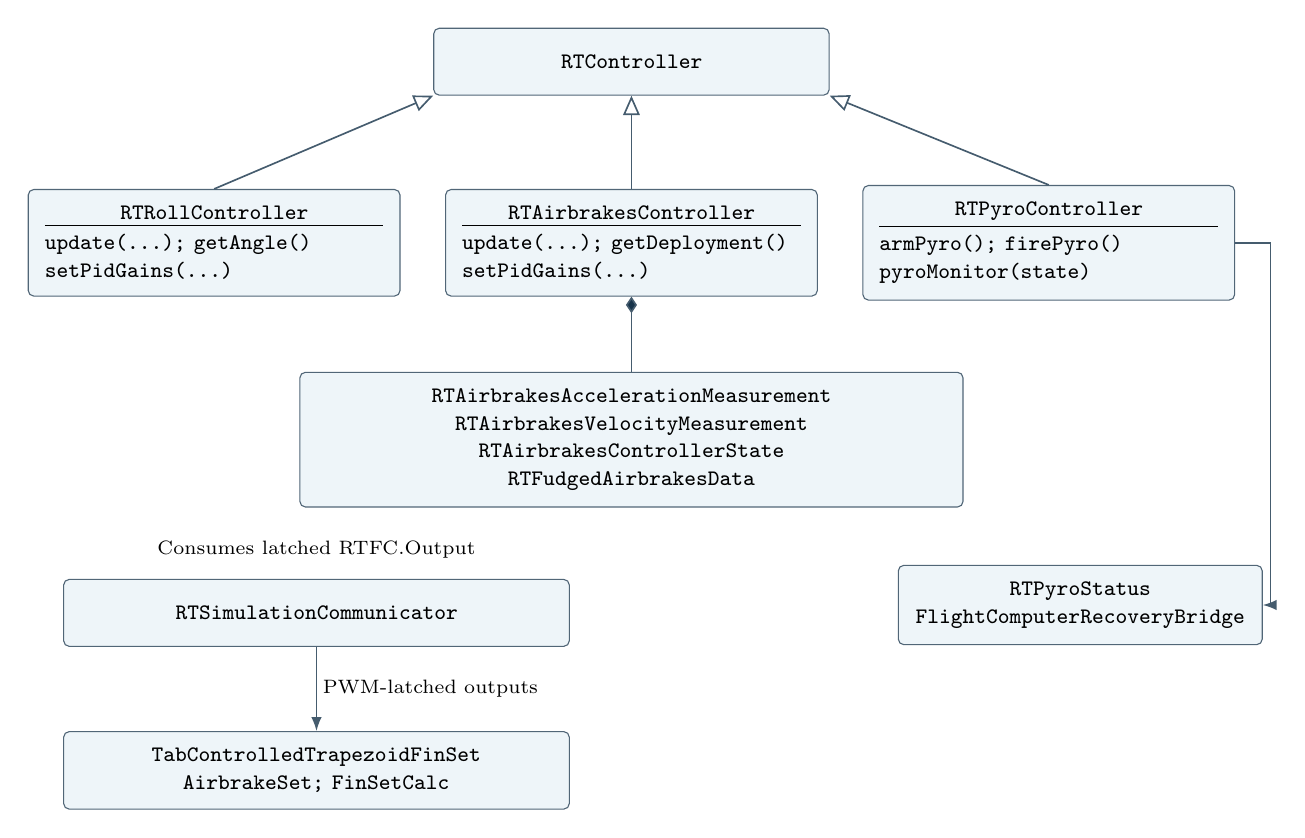
\begin{tikzpicture}
\simple{base}{7.8,0}{RTController}{4.6cm}
\uml{roll}{2.5,-2.3}{RTRollController}{update(...); getAngle()\\setPidGains(...)}{4.3cm}
\uml{brakes}{7.8,-2.3}{RTAirbrakesController}{update(...); getDeployment()\\setPidGains(...)}{4.3cm}
\uml{pyro}{13.1,-2.3}{RTPyroController}{armPyro(); firePyro()\\pyroMonitor(state)}{4.3cm}
\draw[inherit] (roll.north) -- (base.south west);
\draw[inherit] (brakes.north) -- (base.south);
\draw[inherit] (pyro.north) -- (base.south east);
\simple{samples}{7.8,-4.8}{RTAirbrakesAccelerationMeasurement\\RTAirbrakesVelocityMeasurement\\RTAirbrakesControllerState\\RTFudgedAirbrakesData}{8cm}
\draw[own] (brakes) -- (samples);
\simple{status}{13.5,-6.9}{RTPyroStatus\\FlightComputerRecoveryBridge}{4.2cm}
\draw[use] (pyro.east) -- ++(0.45,0) |- (status.east);
\simple{bridge}{3.8,-7}{RTSimulationCommunicator}{6cm}
\simple{fins}{3.8,-9}{TabControlledTrapezoidFinSet\\AirbrakeSet; FinSetCalc}{6cm}
\node[flowlabel] at (3.8,-6.2) {Consumes latched RTFC.Output};

\draw[use] (bridge) -- node[flowlabel,right]{PWM-latched outputs} (fins);
\end{tikzpicture}}

\class{RTSimulationCommunicator} applies latched airbrake fractions and
roll-tab angles to active components in the per-run rocket. FC angles are
degrees; fin geometry uses radians. Named Java writes require exact, unique
rocket component names. Missing FC hardware discards the associated command;
present hardware without a suitable physical binding is diagnosed according
to the binding rules.

Controller blocks use stable component UUIDs for fin tabs, fin cant and
airbrakes. Enabled mapped blocks reserve their outputs even outside their
active states, applying the selected hold/neutral policy. Java broadcasts
skip reserved targets; conflicting explicit named writes are rejected.
State-disjoint blocks may share targets under validated ownership rules.
Actuator movement is ideal at a PWM latch: finite slew, inertia and backlash
are not modeled.

\clearpage
\section{Recovery commands and actual deployment}
\class{RTPyroController} provides six logical channels, arming, firmware status
and pulse timing. An accepted fire command records a sequence, origin and
exact boot time. \class{FlightComputerRecoveryBridge} resolves channel-to-device
UUID assignments and delay, then queues an FC-owned engine event.

\diagram{fig:recovery}{A logical firing command and a physical deployment are distinct events. Engine eligibility checks remain authoritative.}{%
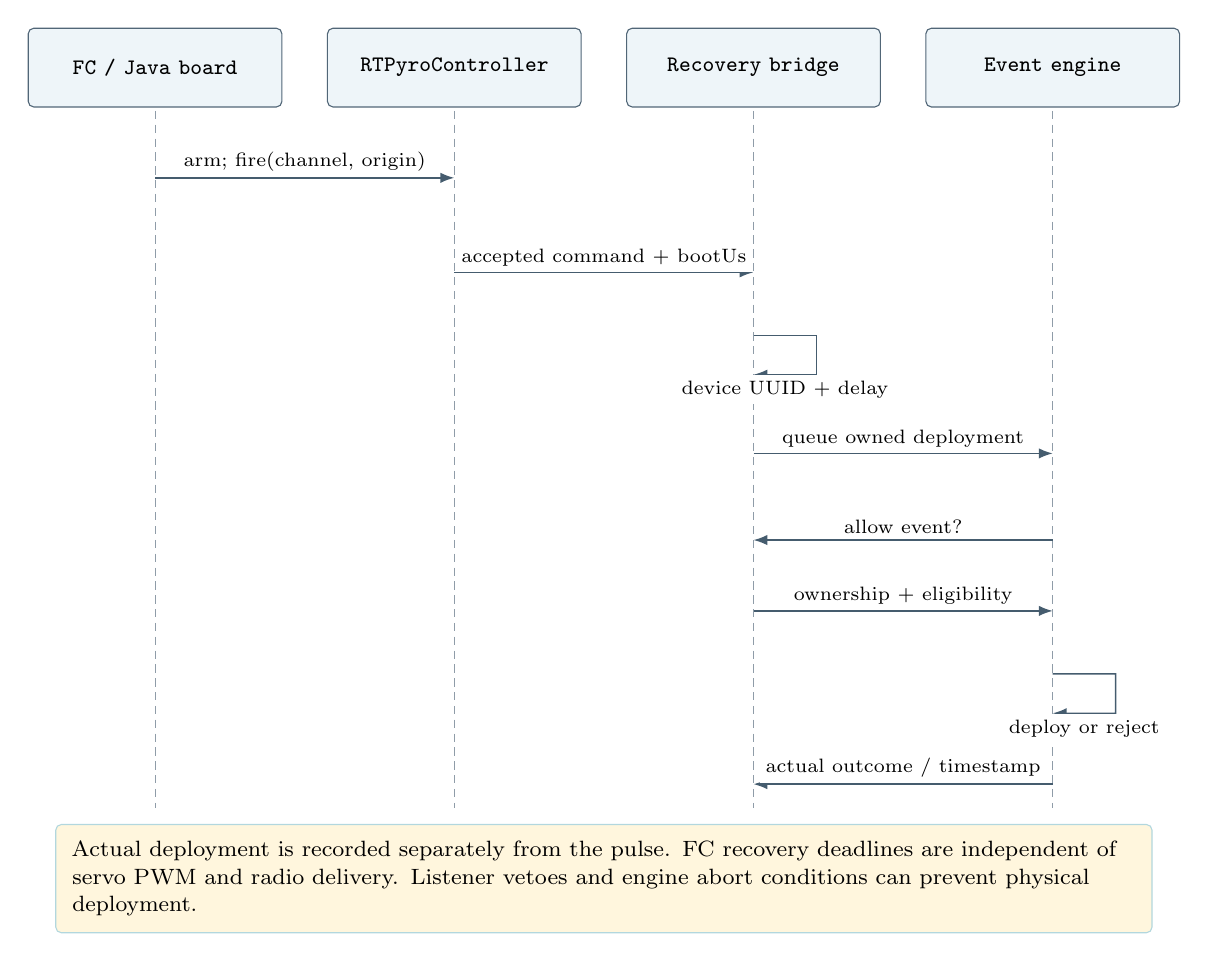
\begin{tikzpicture}
\node[participant,text width=2.8cm] at (1.5,0) {\ttfamily FC / Java board};
\node[participant,text width=2.8cm] at (5.3,0) {\ttfamily RTPyroController};
\node[participant,text width=2.8cm] at (9.1,0) {\ttfamily Recovery bridge};
\node[participant,text width=2.8cm] at (12.9,0) {\ttfamily Event engine};
\foreach \x in {1.5,5.3,9.1,12.9} \draw[lifeline] (\x,-0.55) -- (\x,-9.4);
\draw[use] (1.5,-1.4) -- node[flowlabel,above]{arm; fire(channel, origin)} (5.3,-1.4);
\draw[use] (5.3,-2.6) -- node[flowlabel,above]{accepted command + bootUs} (9.1,-2.6);
\draw[use] (9.1,-3.4) -- ++(0.8,0) -- ++(0,-0.5) -- node[flowlabel,below]{device UUID + delay} (9.1,-3.9);
\draw[use] (9.1,-4.9) -- node[flowlabel,above]{queue owned deployment} (12.9,-4.9);
\draw[use] (12.9,-6.0) -- node[flowlabel,above]{allow event?} (9.1,-6.0);
\draw[use] (9.1,-6.9) -- node[flowlabel,above]{ownership + eligibility} (12.9,-6.9);
\draw[use] (12.9,-7.7) -- ++(0.8,0) -- ++(0,-0.5) -- node[flowlabel,below]{deploy or reject} (12.9,-8.2);
\draw[use] (12.9,-9.1) -- node[flowlabel,above]{actual outcome / timestamp} (9.1,-9.1);
\node[note,text width=13.5cm] at (7.2,-10.3) {Actual deployment is recorded separately from the pulse. FC recovery deadlines are independent of servo PWM and radio delivery. Listener vetoes and engine abort conditions can prevent physical deployment.};
\end{tikzpicture}}

FC-enabled simulation overrides normal OpenRocket deployment rules. Those
saved rules resume when FC simulation is disabled. Physical deployment is
still subject to engine checks, listener vetoes and abort conditions, and is
recorded separately for logs, plots and canopy animation.

The firmware pulse expires using a strict elapsed-millisecond threshold
of more than \(250\ms\). Physical deployment scheduling retains the accepted
command's microsecond timestamp. Continuity affects firmware status reporting;
the \code{firePyro} acceptance gate itself checks arming rather than requiring
simulated continuity.

\clearpage
\section{Telemetry, logging and logical hardware}
\class{RTTelemetryEngine} preserves transmitted packet bytes and decodes them
to ground-station-compatible CSV. Received streams add deterministic packet
loss and delivery delay. \code{OR.log} contains action records and structured
physical/FC plot samples; metadata records paths, settings and completion.

\diagram{fig:telemetry}{Transmitted and received streams, plus the retained logical hardware adapters.}{%
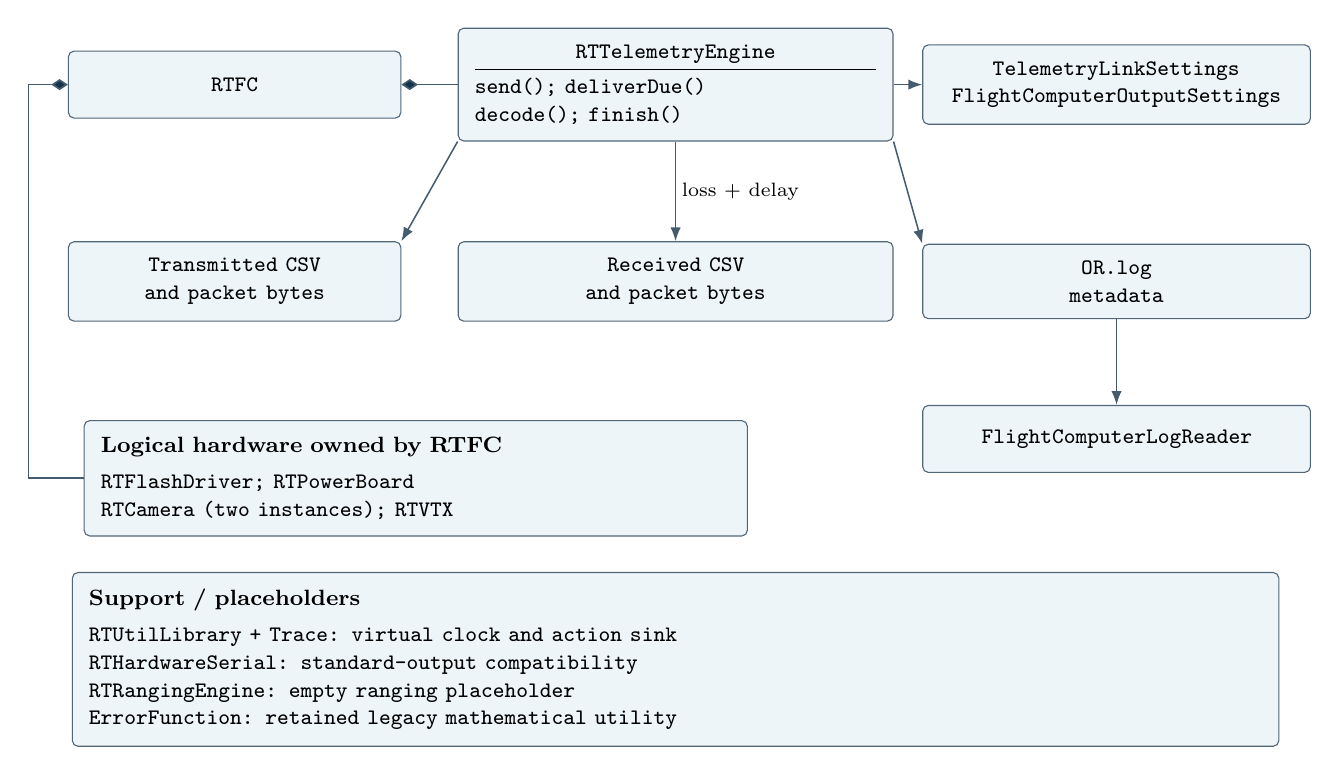
\begin{tikzpicture}
\simple{fc}{2.4,0}{RTFC}{3.8cm}
\uml{telem}{8,0}{RTTelemetryEngine}{send(); deliverDue()\\decode(); finish()}{5.1cm}
\simple{settings}{13.6,0}{TelemetryLinkSettings\\FlightComputerOutputSettings}{4.5cm}
\draw[own] (fc) -- (telem);
\draw[use] (telem) -- (settings);
\simple{tx}{2.4,-2.5}{Transmitted CSV\\and packet bytes}{3.8cm}
\simple{rx}{8,-2.5}{Received CSV\\and packet bytes}{5.1cm}
\simple{log}{13.6,-2.5}{OR.log\\metadata}{4.5cm}
\draw[use] (telem.south west) -- (tx.north east);
\draw[use] (telem) -- node[flowlabel,right]{loss + delay} (rx);
\draw[use] (telem.south east) -- (log.north west);
\simple{replay}{13.6,-4.5}{FlightComputerLogReader}{4.5cm}
\draw[use] (log) -- (replay);
\node[box,text width=8cm] (hardware) at (4.7,-5) {\textbf{Logical hardware owned by RTFC}\\[3pt]
\ttfamily RTFlashDriver; RTPowerBoard\\RTCamera (two instances); RTVTX};
\draw[own] (fc.west) -- ++(-0.5,0) |- (hardware.west);
\node[box,text width=14.9cm] at (8,-7.3) {\textbf{Support / placeholders}\\[3pt]
\ttfamily RTUtilLibrary + Trace: virtual clock and action sink\\
RTHardwareSerial: standard-output compatibility\\
RTRangingEngine: empty ranging placeholder\\
ErrorFunction: retained legacy mathematical utility};
\end{tikzpicture}}

Existing output files are protected against overwrite. Batch and ensemble
members receive distinct output paths. Telemetry is streamed, while result
branches retain plotted samples; short-period traces can still produce large
files. Downlink effects change ground observability, not the closed-loop
physical control calculation.

\class{FlightComputerLogReader} reconstructs available channels and actual
recovery events without executing custom Java from an imported file.
Camera/video, flash and power adapters expose logical operations or nominal
values. They do not model RF propagation, electronics, flash wear or battery
dynamics. The serial wrapper opens no physical serial port.

\clearpage
\section{Designer, persistence and custom programs}
\class{FlightComputerDesign} is the immutable JSON design and validation
boundary. \class{FlightComputerModels} defines hardware capabilities and
defaults. The standard library imports external \code{.fc} files, resolves
references and records behavior fingerprints, excluding presentation-only
names/layout from those fingerprints.

\diagram{fig:designer}{Portable FC definitions, simulation-specific assignments and the graphical editing/runtime connections.}{%
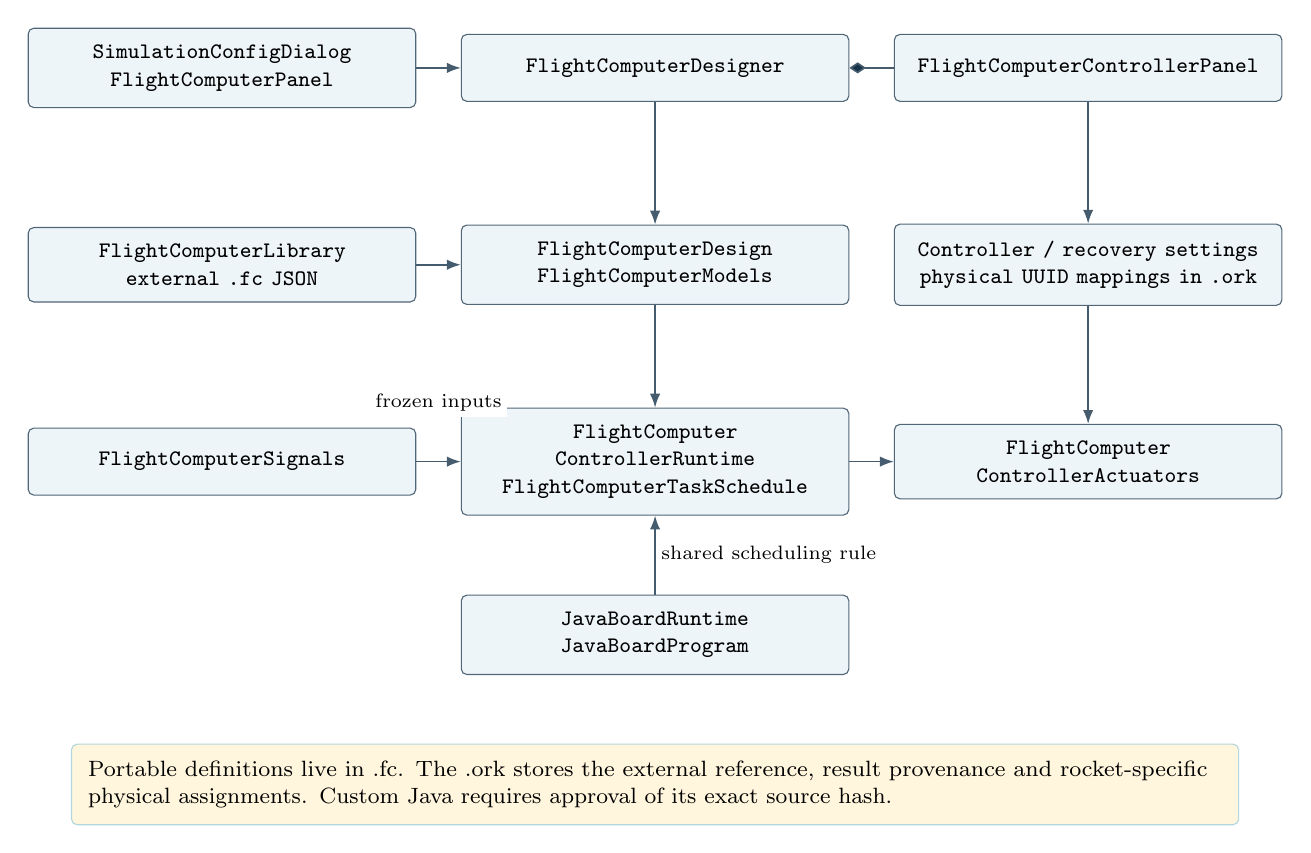
\begin{tikzpicture}
\simple{dialog}{2.5,0}{SimulationConfigDialog\\FlightComputerPanel}{4.5cm}
\simple{designer}{8,0}{FlightComputerDesigner}{4.5cm}
\simple{panel}{13.5,0}{FlightComputerControllerPanel}{4.5cm}
\draw[use] (dialog) -- (designer);
\draw[own] (designer) -- (panel);
\simple{library}{2.5,-2.5}{FlightComputerLibrary\\external .fc JSON}{4.5cm}
\simple{design}{8,-2.5}{FlightComputerDesign\\FlightComputerModels}{4.5cm}
\simple{mapping}{13.5,-2.5}{Controller / recovery settings\\physical UUID mappings in .ork}{4.5cm}
\draw[use] (designer) -- (design);
\draw[use] (library) -- (design);
\draw[use] (panel) -- (mapping);
\simple{signal}{2.5,-5.0}{FlightComputerSignals}{4.5cm}
\simple{runtime}{8,-5.0}{FlightComputer\\ControllerRuntime\\FlightComputerTaskSchedule}{4.5cm}
\simple{actuators}{13.5,-5.0}{FlightComputer\\ControllerActuators}{4.5cm}
\draw[use] (design) -- (runtime);
\draw[use] (signal) -- node[flowlabel,above=16pt]{frozen inputs} (runtime);
\draw[use] (runtime) -- (actuators);
\draw[use] (mapping) -- (actuators);
\simple{java}{8,-7.2}{JavaBoardRuntime\\JavaBoardProgram}{4.5cm}
\draw[use] (java) -- node[flowlabel,right]{shared scheduling rule} (runtime);
\node[note,text width=14.4cm] at (8,-9.1) {Portable definitions live in .fc. The .ork stores the external reference, result provenance and rocket-specific physical assignments. Custom Java requires approval of its exact source hash.};
\end{tikzpicture}}

The simulation's Flight computer tab opens the designer. Hardware, behavior,
Java and controller editors apply snapshot changes with undo/redo. Controller
editing combines algorithm settings, measured-source/quantity selection,
baselines, tuning, timing, states and eligible physical targets.

Custom source derives from \class{JavaBoardProgram}; each run creates fresh
instances. Compilation does not initialize the program class. Execution
requires local approval of the exact source hash and occurs inside the
OpenRocket process, without a sandbox. Independently scheduled boards run
in tandem for algorithm experiments, but do not provide an authoritative
model of inter-board communications.

\clearpage
\section{Results and adjacent simulation improvements}
\class{FlightComputerData} and \class{FlightComputerControllerPlots} record
measured/physical comparisons, servo outputs, controller diagnostics and state.
Digital commands/status use held-value plotting. Structured log metadata
preserves channel identities and units during import.

\diagram{fig:results}{Result paths for FC diagnostics, trajectory animation, ensemble statistics and motor searches.}{%
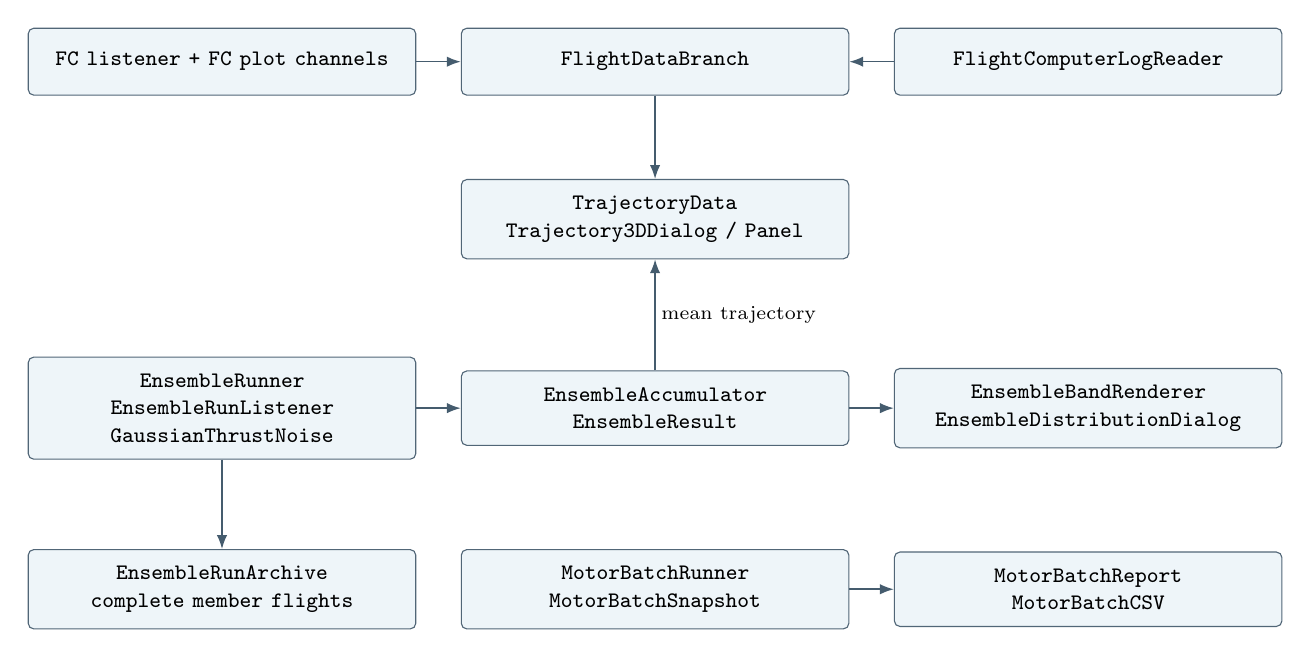
\begin{tikzpicture}
\simple{fc}{2.5,0}{FC listener + FC plot channels}{4.5cm}
\simple{branch}{8,0}{FlightDataBranch}{4.5cm}
\simple{replay}{13.5,0}{FlightComputerLogReader}{4.5cm}
\draw[use] (fc) -- (branch);
\draw[use] (replay) -- (branch);
\simple{trajectory}{8,-2}{TrajectoryData\\Trajectory3DDialog / Panel}{4.5cm}
\draw[use] (branch) -- (trajectory);
\simple{runs}{2.5,-4.4}{EnsembleRunner\\EnsembleRunListener\\GaussianThrustNoise}{4.5cm}
\simple{stats}{8,-4.4}{EnsembleAccumulator\\EnsembleResult}{4.5cm}
\simple{plots}{13.5,-4.4}{EnsembleBandRenderer\\EnsembleDistributionDialog}{4.5cm}
\draw[use] (runs) -- (stats);
\draw[use] (stats) -- (plots);
\draw[use] (stats) -- node[flowlabel,right]{mean trajectory} (trajectory);
\simple{archive}{2.5,-6.7}{EnsembleRunArchive\\complete member flights}{4.5cm}
\draw[use] (runs) -- (archive);
\simple{batch}{8,-6.7}{MotorBatchRunner\\MotorBatchSnapshot}{4.5cm}
\simple{report}{13.5,-6.7}{MotorBatchReport\\MotorBatchCSV}{4.5cm}
\draw[use] (batch) -- (report);
\end{tikzpicture}}

\class{TrajectoryData} reconstructs position, recorded quaternion orientation,
motor burns and recovery events. The cartoon attitude follows that orientation,
not velocity direction. Actual deployment controls the canopy, burn intervals
control exhaust, and FC state labels follow the playhead.

Ensemble engine variation is additive:
\begin{equation}
 T_{\mathrm{member}}(t)=\max\{0,\,T(t)+e(t)\},
 \qquad e(t)\text{ is the configured Gaussian perturbation during burn}.
\end{equation}
Configured atmospheric variation is applied separately. Members are aligned
in physical time to form the mean and sample standard deviation. 2D plots
show mean \(\pm1\sigma\); 3D uses the mean trajectory. Scalar distributions
use each member's extrema/metrics, and the archive retains complete flights.

Motor-batch workers use isolated baseline snapshots, record candidate/delay
outcomes and export CSV. Update and memory helpers are documented maintenance
utilities, rather than FC runtime dependencies.

\clearpage
\section{Complete firmware class index}
All entries below are beneath \code{edu.mit.rocket_team}. The generated
Javadoc gives the complete method-level API, including private members.
The index includes legacy and placeholder classes so their presence is not
mistaken for active physical hardware simulation.

\small
\begin{longtable}{@{}>{\raggedright\arraybackslash}L{5.65cm}>{\raggedright\arraybackslash}L{2.1cm}>{\raggedright\arraybackslash}L{7.4cm}@{}}
\toprule Class & Subpackage & Responsibility\\\midrule
\endfirsthead
\toprule Class & Subpackage & Responsibility (continued)\\\midrule
\endhead
\bottomrule
\endfoot
\class{RTCamera} & \code{AV} & Logical camera setup; two instances are owned by the FC.\\
\class{RTVTX} & \code{AV} & Logical video-transmitter power requests.\\
\class{FlightComputerTimingSettings} & \code{FC} & Read/work/jitter costs, PWM phase and timing seed.\\
\class{RTFC} & \code{FC} & Translated sketch, loop phases, state actions and PWM snapshots.\\
\class{RTPyroController} & \code{control} & Six-channel arm/fire, pulse and status logic.\\
\class{RTRollController} & \code{control} & Firmware roll PID and aerodynamic gain schedule.\\
\class{RTAirbrakesAccelerationMeasurement} & \code{control.}\newline\code{airbrakes} & Acceleration/time sample for the coast fit.\\
\class{RTAirbrakesController} & \code{control.}\newline\code{airbrakes} & Included coast predictor and airbrake control sequence.\\
\class{RTAirbrakesControllerState} & \code{control.}\newline\code{airbrakes} & Predictor preparation and control phase enumeration.\\
\class{RTAirbrakesVelocityMeasurement} & \code{control.}\newline\code{airbrakes} & Velocity/time sample for the coast fit.\\
\class{RTAccel} & \code{instrument} & Fresh-sample consumption and longitudinal velocity integration.\\
\class{RTBaro} & \code{instrument} & Pressure altitude, moving average, zeroing and maximum tracking.\\
\class{RTGPS} & \code{instrument} & Held GPS fix, quantization, relative height and maximum tracking.\\
\class{RTGyro} & \code{instrument} & Angular-rate integration and firmware attitude conventions.\\
\class{RTMag} & \code{instrument} & Legacy magnetometer/roll injection adapter.\\
\class{RTFlashDriver} & \code{internal} & Logical logging allocation and packet append operations.\\
\class{RTPowerBoard} & \code{internal} & Nominal power values, converter enables and protection flags.\\
\class{FlightComputerOutputSettings} & \code{telemetry} & CSV/log paths and distinct multi-run filenames.\\
\class{RTRangingEngine} & \code{telemetry} & Reserved empty ranging placeholder.\\
\class{RTTelemetryEngine} & \code{telemetry} & Byte queues, loss/delay, packet decoding and streamed files.\\
\class{TelemetryLinkSettings} & \code{telemetry} & Reproducible downlink configuration.\\
\pagebreak
\class{ErrorFunction} & \code{util} & Legacy error-function and normal-distribution approximations.\\
\class{RTController} & \code{util} & Common setup, loop and injection interface for controllers.\\
\class{RTInstrument} & \code{util} & Instrument base sharing the run-local clock and trace.\\
\class{RTRocketState} & \code{util} & Firmware phase codes used by commands and telemetry.\\
\class{RTSimulationCommunicator} & \code{util} & Latched commands to per-run airbrakes and tab fins.\\
\class{RTUtilLibrary} & \code{util} & Unsigned clock arithmetic, nested Trace and orientation helpers.\\
\class{RTAccelData} & \code{util.data} & Mutable sensor-axis specific-force payload.\\
\class{RTBaroData} & \code{util.data} & Barometer engineering values and optional raw ADC fields.\\
\class{RTFudgedAirbrakesData} & \code{util.data} & Legacy predictor altitude/velocity/acceleration/apogee inputs.\\
\class{RTFudgedData} & \code{util.data} & Shared marker base for injected payloads.\\
\class{RTGPSData} & \code{util.data} & Coordinates, MSL altitude, fix and dilution-of-precision values.\\
\class{RTGyroData} & \code{util.data} & Mutable angular-rate payload.\\
\class{RTMagData} & \code{util.data} & Legacy magnetometer and supplied roll payload.\\
\class{RTPyroStatus} & \code{util.data} & Two-bit firmware continuity/firing status enumeration.\\
\class{RTHardwareSerial} & \code{util.}\newline\code{hardware} & Standard-output compatibility for firmware serial calls.\\
\end{longtable}
\normalsize

\clearpage
\section{Build, regeneration and verification}
The code scope and context classes are defined by two manifests within the
Gradle project:
\begin{lstlisting}
config/mit-documentation-sources.txt
config/mit-javadoc-connectors.txt
\end{lstlisting}
From \code{clone/openrocket-release-24.12.RC.01}, with JDK 17:
\begin{lstlisting}[language=bash]
./gradlew formatMitJava
./gradlew verifyMitJavadoc rocketTeamJavadoc
./gradlew shadowJar
\end{lstlisting}
Run formatting before compilation or documentation generation, not
concurrently. The formatter is pinned to google-java-format 1.24.0 with
four-space indentation and preservation of import order, unused imports and
string literals. Documentation dependencies are developer-only.

\code{verifyMitJavadoc} uses the JDK parser to audit every explicit method and
constructor in the improvement manifest, including private methods, test
helpers and anonymous callbacks. It fails on a missing description.
\code{rocketTeamJavadoc} includes private members and selected engine types,
and checks comment syntax and links. Missing field descriptions in upstream
classes are excluded from warnings; the separate method audit is not disabled.

\subsection{Maintaining the incorporated chapter}
The chapter is now \code{sections/08-flight-computer.tex}. Compile the complete guide through \code{main.tex}, as described in Chapter~\ref{ch:build}. Its nine figures remain native TikZ. The original standalone source in \code{reference/} retains its original build instructions; it is a historical copy, not an additional input to the guide. The Markdown/UML/Javadoc tasks in the source repository remain separate from this document build.

\subsection{Recorded validation results}
\begin{itemize}
\item \textbf{1,560/1,560 explicit methods and constructors documented} across
150 original improvement files and the new parser/audit utility.
\item \textbf{150/150 original scoped files} retain their executable Java
tokens after comment/spacing removal and namespace normalization.
\item \textbf{148 core tests and 65 Swing/UI tests passed}, with no failures,
errors or skipped tests. Coverage includes firmware replay, microsecond
scheduling, PWM ties, recovery, independent actuators, controller blocks,
ensembles, motor batches, plots, editor lifetime and update routing.
\item \textbf{Root shadow JAR rebuilt successfully}. The startup class and
\code{edu/mit/rocket_team/FC/RTFC.class} are present; no entries remain beneath
the old namespace.
\item \textbf{Javadoc generated successfully} with documentation/link checks.
All 36 top-level firmware classes are represented by this report's figures
and complete class index.
\end{itemize}

Historically verified application artifact: \code{build/libs/OpenRocket-MIT-v6.4.jar}, with its
checksum and installed-app compatibility alias. Restart an already-running
application to load the renamed classes.

\clearpage
\section{Source map and limits of the model}
The main integration entry points, relative to the Gradle project, are:
\begin{lstlisting}
core/src/main/java/edu/mit/rocket_team/
core/src/main/java/info/openrocket/core/simulation/
  listeners/FlightControllerSimulatorListener.java
  extension/impl/ZephyrusFlightComputer.java
  flightcomputer/
swing/src/main/java/info/openrocket/swing/gui/
  flightcomputer/
  simulation/FlightComputerPanel.java
\end{lstlisting}
The connected framework types include \class{Simulation}, the two event
engines, \class{SimulationStatus}, \class{SimulationConditions},
\class{SimulationOptions}, the stepper/listener interfaces and helpers,
\class{FlightDataBranch}, \class{FlightEvent}, \class{FinSetCalc}, controlled
fins, airbrakes and \class{RecoveryDevice}.

\begin{table}[htbp]\centering\small
\begin{tabularx}{\linewidth}{@{}L{3.7cm}Y@{}}\toprule
Area & What the implementation establishes\\\midrule
Virtual scheduling & Deterministic ordering, acquisition age, completion delay and PWM/recovery deadlines for the configured model.\\
Processor and buses & User-supplied execution costs; no authoritative shared-CPU or inter-board communications model.\\
Sensors & Engineering-unit acquisition, noise/bias, rotation and firmware filtering; not complete sensor electronics.\\
Servos and aerodynamics & Commands reach physical fin/airbrake models; no modeled servo dynamics or general qualification of high-deflection aerodynamics.\\
Recovery & Accepted logical commands connect to actual engine deployment events, subject to eligibility and abort rules.\\
Radio and power & Packet loss/delay and logical/nominal hardware behavior; not RF, battery or electrical dynamics.\\
\bottomrule\end{tabularx}
\caption{Implementation contracts and their practical limits.}
\end{table}

\subsection{Companion documents}
Within \code{doc/improvements}, the recovery implementation is described in
\code{11-flight-computer-recovery-implementation.md}; controller behavior,
ownership, tuning and verification are described in
\code{13-flight-computer-controller-implementation.md}. The browsable method
reference begins at \code{javadoc/index.html}.

Repository: \href{https://github.com/MDNich/ActiveControl_MIT_RktTeam}{github.com/MDNich/ActiveControl\_MIT\_RktTeam}.
The report describes the 6.4 implementation verified on 11 October 2026.
Diagrams are curated architecture views and must be updated when source
relationships or scheduling order change.

\chapter{Simulation configurations and batch workflows}\label{ch:workflows}
\section{Three different meanings of configuration}
An OpenRocket design can carry multiple motor and staging arrangements, multiple experiments on those arrangements, and multiple random realizations of an experiment. Keeping these levels separate is essential when extending the application.

\begin{tabularx}{\linewidth}{@{}L{3.5cm}YY@{}}\toprule
Object & What it selects & What it does not own\\\midrule
\class{FlightConfiguration} & A configuration ID, active stages, installed motors, and configuration-dependent component parameters & Weather, integrator settings, or recorded trajectories\\
\class{Simulation} and \class{SimulationOptions} & One selected flight configuration plus launch conditions, models, timing, extensions, and ensemble settings & A separate editable copy of the entire design for every saved simulation\\
\class{SimulationConditions} & Runtime calculators, listeners, configuration, and environment prepared for one execution & The GUI's editable settings model\\
\class{EnsembleRunParameters} & The particular environmental and coefficient draws, motor seed, and wind bearing for one member & A second independent ensemble nested inside the member\\\bottomrule
\end{tabularx}

The saved simulation is the experiment's durable handle. It links the design and settings to its latest result. A run translates editable options into runtime conditions and creates mutable execution state. The numerical engine described in Chapter~\ref{ch:engine} consumes this prepared state; it does not reach into Swing controls to obtain values.

Changing design geometry, flight configuration, relevant options, or extension configuration can make a result stale. The fork also tracks flight-computer design provenance and fingerprints. A historical result remains evidence of the settings that produced it, even when the current editor shows different settings. Imported external data has its own status and must not be mistaken for a newly executed simulation.

\sourceline{\source{core/src/main/java/info/openrocket/core/document/Simulation.java}{Simulation}; \source{core/src/main/java/info/openrocket/core/simulation/SimulationOptions.java}{SimulationOptions}; \source{core/src/main/java/info/openrocket/core/simulation/SimulationConditions.java}{SimulationConditions}.}

\section{Configuring an ordinary flight}
Before any batch or control feature is involved, a simulation specifies a vehicle configuration and a launch experiment. The flight-configuration ID selects the motor installations and configuration-specific ignition, separation, and deployment settings in the component tree. The simulation options then provide the launch site, guide, environment, and numerical controls. Two simulations can select the same motors and differ only in weather; two configurations can install different motors while using otherwise identical launch conditions.

\begin{tabularx}{\linewidth}{@{}L{3.1cm}YY@{}}\toprule
Setting family & What it controls & Consequence in the execution path\\\midrule
Launch site & Latitude, longitude, altitude and geodetic method & Initial world position, gravity, atmospheric altitude, coordinate propagation, and optional Coriolis terms\\
Launch guide & Length, inclination and bearing & Initial attitude and constrained travel before rod clearance\\
Atmosphere & Standard atmosphere or launch temperature/pressure & Density, speed of sound and viscosity evaluated along the flight\\
Wind & Average/turbulent or altitude-dependent wind settings and seed & Air-relative velocity, angle of attack and drift; the wind is not simply added to ground speed after integration\\
Numerics & Maximum timestep, angular-step limits and maximum simulation duration & Resolution, event handling and run termination; a smaller maximum step is not itself a new physical model\\
Extensions & Selected features and their saved settings & Runtime listener initialization and extra data channels\\\bottomrule
\end{tabularx}

Defaults for a newly created simulation come from application preferences. Once a scenario has its own options, those are the inputs to its next run. The status displayed beside a simulation distinguishes an unrun case, usable stored data, stale data, imported data, and execution problems. Reusing a result is therefore a decision about the saved definition and its provenance, not merely whether an array of samples exists.

Motor selection also includes ejection delay and ignition policy. A curve's manufacturer/designation describes the motor record, while the installation associates that record with a mount and flight configuration. A clustered mount can produce several motor instances from one configuration entry. The motor chooser, configuration tables, and simulation options edit these different owners rather than merging them into one global motor selection.

\sourceline{\source{core/src/main/java/info/openrocket/core/simulation/SimulationOptions.java}{ordinary simulation options}; \source{core/src/main/java/info/openrocket/core/rocketcomponent/FlightConfiguration.java}{flight configuration}; \source{core/src/main/java/info/openrocket/core/motor/MotorConfiguration.java}{motor installation}.}

\section{Static component analysis and parameter sweeps}\label{sec:static-analysis}
The inherited component-analysis tools explain why the current design has a particular mass, CP, drag coefficient, or roll contribution. They ask the same mass and aerodynamic calculators used elsewhere for a decomposition by component. This is useful before running a trajectory: a large pressure contribution can be traced to a shape or exposed junction, while an unexpected CG can be traced to a material, motor, instance count, or override.

\class{CAParameters} holds the analysis conditions. \class{CAParameterSweep} copies those conditions, varies Mach number, angle of attack, lateral wind/flow angle, or roll rate, constructs \class{FlightConditions}, and asks the aerodynamic calculator for force analysis at every point. \class{CADataBranch} stores the domain values and per-component channels; \class{CADataType} and \class{CADomainDataType} describe the quantities and units. The Swing analysis dialog supplies component selection, tables, plots, and export.

These are controlled static evaluations. Sweeping Mach at fixed angle of attack does not integrate a trajectory through increasing speed, burn propellant, or fly the vehicle through a wind profile. The sweep constructs flight conditions from the selected rocket configuration and analysis parameters; it does not automatically reproduce every atmospheric setting of an arbitrary saved simulation. A comparison with a flight-history sample must align the relevant conditions explicitly.

CP and normal-force slope are related: the combined CP is weighted by component normal-force contributions. A negligible total weighting makes a CP undefined, rather than establishing a meaningful CP at the origin. Static stability is conventionally the axial separation $x_{\rm CP}-x_{\rm CG}$; dividing by reference diameter expresses it in calibers. Motor loading, reference diameter, flow angle, and Mach can change the result. A positive static margin is not a complete prediction of dynamic stability throughout a flight.

Drag analysis distinguishes pressure, base, and friction terms and the distinction between a component's per-instance value and the installed total. A single tree entry can represent several fins, lugs, or repeated assemblies. The mass-analysis map similarly retains contributions and override information rather than treating every row as an unrelated lump.

\begin{contract}
In this snapshot, \class{CAParameterSweep} forms its channel named \code{TOTAL_ROLL_COEFFICIENT} by adding the forcing and damping values. The flight engine's net roll term subtracts damping from forcing. Therefore that analysis channel must not be identified with the engine's net torque coefficient without checking the sign convention. The separate forcing and damping channels are the unambiguous comparison points.
\end{contract}

\sourceline{\source{core/src/main/java/info/openrocket/core/componentanalysis/CAParameterSweep.java}{CAParameterSweep}; \source{core/src/main/java/info/openrocket/core/componentanalysis/CADataBranch.java}{CADataBranch}; \source{swing/src/main/java/info/openrocket/swing/gui/dialogs/componentanalysis/ComponentAnalysisDialog.java}{component-analysis dialog}; \source{core/src/main/java/info/openrocket/core/masscalc/CMAnalysisEntry.java}{mass-analysis entries}.}


\section{Ensemble execution and ownership}
An ensemble repeats an experiment with controlled variation. \class{EnsembleSettings} contains the count, seed, worker limit, and distributions; \class{EnsembleRunner} coordinates members; \class{EnsembleRunListener} applies the member's runtime perturbations; \class{EnsembleAccumulator} produces aggregate statistics; and \class{EnsembleRunArchive} retains compressed individual flights.

\diagram{fig:ensemble}{An ensemble isolates member execution, consumes members in a deterministic order, and publishes a complete result.}{
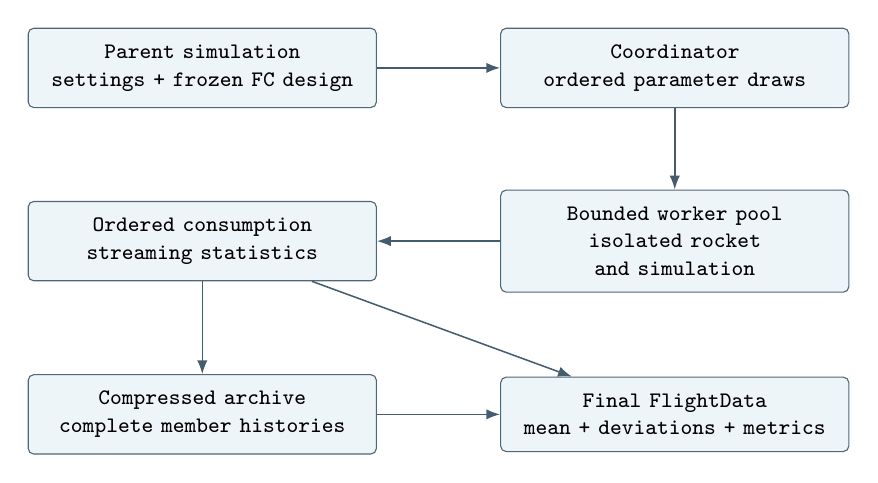
\begin{tikzpicture}
\simple{parent}{0,0}{Parent simulation\\settings + frozen FC design}{4cm}
\simple{draw}{6,0}{Coordinator\\ordered parameter draws}{4cm}
\simple{members}{6,-2.2}{Bounded worker pool\\isolated rocket and simulation}{4cm}
\simple{acc}{0,-2.2}{Ordered consumption\\streaming statistics}{4cm}
\simple{archive}{0,-4.4}{Compressed archive\\complete member histories}{4cm}
\simple{publish}{6,-4.4}{Final FlightData\\mean + deviations + metrics}{4cm}
\draw[use] (parent)--(draw); \draw[use] (draw)--(members);
\draw[use] (members)--(acc); \draw[use] (acc)--(archive);
\draw[use] (acc)--(publish); \draw[use] (archive)--(publish);
\end{tikzpicture}}

Each member receives a copied rocket with component IDs preserved, a separate document and simulation, its chosen flight configuration, its own random seed, and cloned listeners. The child has ensemble execution disabled. Preserving IDs lets recovery and actuator assignments resolve against the copied geometry; preserving IDs does not imply sharing the component instances.

The coordinator makes random draws in member order before handing work to the pool. Wind/atmosphere/motor choices, coefficient perturbations, and wind-bearing perturbations use the intended random streams so adding a new category need not silently scramble unrelated draws. Results are consumed in member order even if workers finish out of order. This makes aggregate arithmetic reproducible across worker counts and bounds the number of live, uncompressed histories by the worker window. Compressed archives still grow with the amount of retained data.

The default worker count is four; validated settings can select another count, capped at 256 and reduced to the number of runs. Parallel execution rejects simulation extensions other than the specifically supported flight-computer extension. This is a concrete compatibility rule: cloning an arbitrary extension is not proof that its static state or external resources are thread safe. The selected external FC design is frozen for the ensemble so a file edit midway through the run cannot change later members.

Cancellation interrupts workers and closes the executor and archive-building work. The parent publishes an ensemble only after the requested members have produced a valid complete result. A failed, aborted, or structurally inconsistent member is not silently omitted from the denominator.

\section{What an ensemble varies}
Member parameters include launch temperature and pressure, east/north wind components, wind bearing, a motor-noise seed, and multiplicative mass, drag, roll-force, and roll-damping factors. A coefficient draw has the form $m=1+\sigma Z$, with $Z$ a standard normal variate. Factors that must be positive are validated; invalid realizations are rejected rather than clipped into an artificial point mass at zero. Disabled variations reduce to the nominal values and unit multipliers.

The mass and aerodynamic perturbations are applied through simulation callbacks. They express uncertainty in the evaluated model; they are not a permanent edit to the user's component tree. A coefficient multiplier is also a different hypothesis from changing a geometric dimension and recomputing all dependent properties. The settings report should preserve which hypothesis was selected.

\class{GaussianThrustNoise} is evaluated from seeded knots indexed by physical time and motor identity. It is not a new random number on every Runge--Kutta derivative call. Adjacent normal samples are interpolated and divided by $\sqrt{(1-f)^2+f^2}$, where $f$ is the interpolation fraction, preserving marginal variance during interpolation. The resulting process is time-correlated, with its behavior set by the knot spacing. During the burn, noisy thrust is clamped to a nonnegative value. During thrusting, the ensemble limiter caps a step at one quarter of the configured noise interval. Internal RK evaluations and worker scheduling do not advance a mutable random stream differently.

\sourceline{\source{core/src/main/java/info/openrocket/core/simulation/ensemble/EnsembleSettings.java}{EnsembleSettings}; \source{core/src/main/java/info/openrocket/core/simulation/ensemble/EnsembleRunner.java}{EnsembleRunner}; \source{core/src/main/java/info/openrocket/core/simulation/ensemble/EnsembleRunListener.java}{EnsembleRunListener}; \source{core/src/main/java/info/openrocket/core/simulation/ensemble/GaussianThrustNoise.java}{GaussianThrustNoise}.}

\section{Statistics, alignment, and interpretation}
Member timesteps need not coincide. The accumulator starts with the first member's time grid and restricts output to the physical-time interval common to all members, including their ground-hit limits. It aligns subsequent channels onto that grid and tracks streaming moments. Continuous scalar channels use their corresponding interpolated values; discrete and special channels require their own treatment. A missing value is not substituted with zero.

Ordinary scalar bands describe the sample standard deviation, with the $n-1$ denominator, around the ensemble mean. Wrapped angles use circular treatment. Quaternion samples are aligned to a common hemisphere to avoid cancellation between $q$ and $-q$; the playback reader normalizes the component mean before using it as an orientation. A mixed FC state is marked mixed, not presented as an intermediate state-machine state. Recovery channels can express the fraction of members deployed at a particular physical time. These summaries answer different questions and should not be plotted as if they all had ordinary continuous semantics.

Only matching events present in all members enter the mean event series, at their average time, and only inside the common output interval. Scalar metrics such as each member's apogee are collected from individual full flights. Thus the average of member apogees is not generally the peak of the mean altitude curve. Individual archived histories remain available beyond the common interval, so a shorter member does not destroy the longer member's descent record.

\begin{contract}
An ensemble is a model-based sensitivity experiment. Its bands reflect the selected distributions and shared model assumptions. They are not automatically calibrated confidence intervals for a real vehicle, and a mean trajectory is not a trajectory flown by a particular member.
\end{contract}
\sourceline{\source{core/src/main/java/info/openrocket/core/simulation/ensemble/EnsembleAccumulator.java}{EnsembleAccumulator}; \source{core/src/main/java/info/openrocket/core/simulation/ensemble/EnsembleResult.java}{EnsembleResult}; \source{core/src/main/java/info/openrocket/core/simulation/ensemble/EnsembleRunArchive.java}{EnsembleRunArchive}.}

\section{Motor comparison batches}
Motor comparison asks how a fixed design behaves with different candidate motors. It is a separate workflow from random variation of one motor. The GUI gathers a baseline simulation, motor mount, candidate filters, constraints, and delay policy into a snapshot. \class{MotorCandidateSelector} filters the motor database; \class{MotorClearance} checks fit and intersections; \class{MotorBatchRunner} executes isolated cases; metric and report classes retain the outcome of each case.

Filters cover dimensions and motor characteristics such as manufacturer, impulse, thrust, burn duration, and certification information. Diameter fit and geometric intersections are distinct checks. An overlength motor can be represented as an advisory case rather than categorically excluded; an intersecting installation requires the workflow's explicit override and retains its warning. This distinction allows intentional motor protrusion without hiding collisions with other components.

The runner uses a bounded pool, copies the baseline for individual cases, applies the chosen motor and delay, and records failures alongside successful results. The listed-delay search evaluates candidate delays and ranks eligible outcomes using deployment metrics. A batch report is not the same object as an ensemble mean: it is a comparison table whose rows keep their motor identities, warnings, constraints, and outcomes. Selected results can become ordinary simulations for further inspection. CSV exports and saved report history support reviewing the comparison after the worker has finished.

\sourceline{\source{core/src/main/java/info/openrocket/core/simulation/motorbatch/MotorBatchSnapshot.java}{MotorBatchSnapshot}; \source{core/src/main/java/info/openrocket/core/simulation/motorbatch/MotorCandidateSelector.java}{MotorCandidateSelector}; \source{core/src/main/java/info/openrocket/core/simulation/motorbatch/MotorClearance.java}{MotorClearance}; \source{core/src/main/java/info/openrocket/core/simulation/motorbatch/MotorBatchRunner.java}{MotorBatchRunner}; \source{swing/src/main/java/info/openrocket/swing/gui/simulation/MotorBatchDialog.java}{MotorBatchDialog}.}

\section{Design optimization}
The inherited optimization framework changes selected design variables to improve an objective. \class{SimulationModifier} implementations define the variables and their ranges. An \class{OptimizableParameter} extracts a quantity from the trial design or simulated result, while an \class{OptimizationGoal} converts it into a minimization objective. Domain constraints penalize unacceptable trial designs. The numerical search layer supplies algorithms independently of the rocket-specific objective adapter.

\class{RocketOptimizationFunction} duplicates the rocket and simulation for an evaluation, applies the trial modifiers, checks the domain, and evaluates the requested quantity. The GUI's optimization worker coordinates progress and plots. A one-variable search and a multidimensional search can use different algorithms without teaching the flight engine how optimization works.

These workflows can share design and result types, but their semantics differ: an ordinary simulation predicts one configured flight; an ensemble summarizes randomized members; a motor batch compares named alternatives; an optimizer searches a variable space. New UI or export code should retain that distinction rather than flattening all four into an undifferentiated list of trajectories.
\sourceline{\source{core/src/main/java/info/openrocket/core/optimization/rocketoptimization/RocketOptimizationFunction.java}{RocketOptimizationFunction}; \source{core/src/main/java/info/openrocket/core/optimization/services/OptimizationServiceHelper.java}{OptimizationServiceHelper}; \source{swing/src/main/java/info/openrocket/swing/gui/dialogs/optimization/GeneralOptimizationDialog.java}{GeneralOptimizationDialog}.}

\section{Optimization variables, goals, and search mechanics}
The optimization services offer a bounded set of meaningful design variables. The default modifier service includes nose and transition dimensions, body-tube dimensions, fin chords/span/sweep/cant where supported, launch-lug dimensions, explicit component mass, parachute diameter and drag coefficient, and streamer dimensions/aspect ratio/drag coefficient. Availability depends on component type, automatic sizing, fill state, and whether a coefficient is automatic. It avoids offering incompatible parameterizations indiscriminately, such as two independent controls for quantities already linked by geometry.

\class{GenericComponentModifier} targets a component by identity and applies a property change through the appropriate model API. Configuration modifiers handle values associated with a flight configuration. The search variables have physical bounds and display units, but the numerical optimizer operates in its own normalized variable space. A variable being offered in the dialog does not mean the search can violate the underlying component's geometry constraints.

Objective services include maximum altitude, speed and acceleration; absolute or relative stability; impact velocity; landing distance; flight time; and deployment velocity. Some quantities can be obtained from static calculations, while trajectory objectives require a simulation. A minimization goal preserves the objective direction, a maximization goal reverses it for the minimizer, and a value-seeking goal rewards proximity to a target. The stability domain can restrict acceptable designs; the identity domain supplies no such additional restriction.

The general optimizer layer contains one-dimensional golden-section search and multidirectional search for several variables, along with points, controllers, caches, and stopping/progress interfaces. Those classes know about functions and evaluations, not nose cones or launch rods. \class{RocketOptimizationFunction} is the adapter that copies the design, applies modifiers, checks the domain, and evaluates the requested physical quantity. The GUI worker presents progress and candidate designs without running the search on Swing's event-dispatch thread.

The returned design is the search result for the selected variables, bounds, goal, and model. It does not imply a global optimum over all possible rocket shapes, especially when the feasible region is constrained or the objective is irregular. Optimization also differs from an uncertainty ensemble: searching for a high apogee does not estimate the spread of apogees under uncertain conditions.

\sourceline{\source{core/src/main/java/info/openrocket/core/optimization/services/DefaultSimulationModifierService.java}{available modifiers}; \source{core/src/main/java/info/openrocket/core/optimization/rocketoptimization/modifiers/GenericComponentModifier.java}{component modifier}; \source{core/src/main/java/info/openrocket/core/optimization/rocketoptimization/domains/StabilityDomain.java}{stability domain}; \source{core/src/main/java/info/openrocket/core/optimization/general/onedim/GoldenSectionSearchOptimizer.java}{golden-section search}; \source{core/src/main/java/info/openrocket/core/optimization/general/multidim/MultidirectionalSearchOptimizer.java}{multidirectional search}.}


\chapter{Desktop GUI and editing workflows}\label{ch:gui}
\section{Windows, panels, and model ownership}
The desktop is a Swing application. A \class{BasicFrame} presents an \class{OpenRocketDocument}; panels and dialogs edit or display that document and its simulations. The core module owns vehicle, configuration, numerical, and persistence concepts. Swing owns widgets, selection, layout, dialogs, rendering, progress, and user interaction. The separation lets a simulation run without a visible editor and keeps unit conversion and display preferences out of physical equations.

\diagram{fig:gui}{The GUI edits durable models and launches workers; it reads results after execution.}{
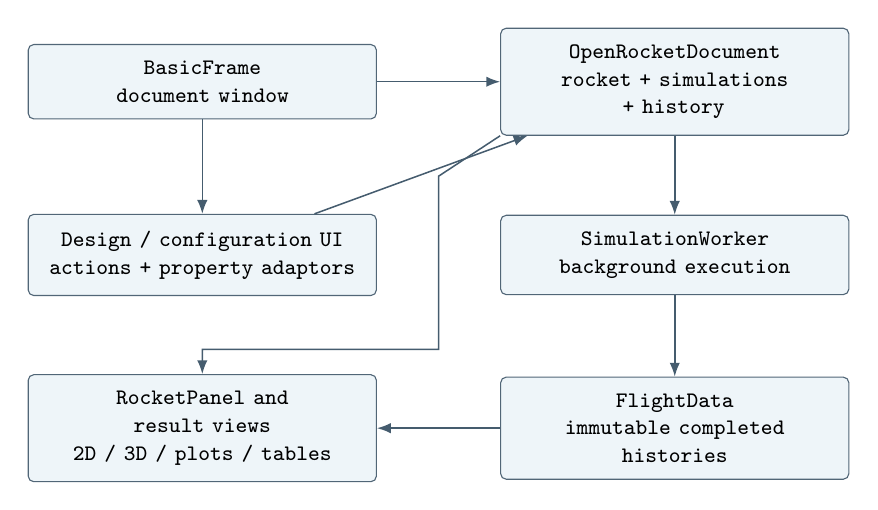
\begin{tikzpicture}
\simple{frame}{0,0}{BasicFrame\\document window}{4cm}
\simple{doc}{6,0}{OpenRocketDocument\\rocket + simulations + history}{4cm}
\simple{edit}{0,-2.2}{Design / configuration UI\\actions + property adaptors}{4cm}
\simple{worker}{6,-2.2}{SimulationWorker\\background execution}{4cm}
\simple{view}{0,-4.4}{RocketPanel and result views\\2D / 3D / plots / tables}{4cm}
\simple{data}{6,-4.4}{FlightData\\immutable completed histories}{4cm}
\draw[use] (frame)--(doc); \draw[use] (frame)--(edit);
\draw[use] (edit)--(doc); \draw[use] (doc)--(worker);
\draw[use] (worker)--(data); \draw[use] (data)--(view);
\draw[use] (doc.south west) -- (3,-1.2) -- (3,-3.4) -| (view.north);
\end{tikzpicture}}

The design area combines a component hierarchy, component actions, configuration controls, and a rendered rocket. Tree selection and figure selection identify the same underlying components. The flight-configuration panel changes the selected motor/stage arrangement. The simulation panel manages named experiments and their statuses; it does not itself integrate the equations of motion.

Component dialogs are specialized because a transition, motor mount, fin set, parachute, and airbrake expose different physical parameters. Common controls reuse adaptors such as \class{DoubleModel} and \class{BooleanModel}. An adaptor connects a property getter/setter to a spinner, slider, checkbox, units, limits, and change notifications. The setter remains responsible for model invariants and change events. A widget displaying millimeters must ultimately set the corresponding SI-valued model property.

\sourceline{\source{swing/src/main/java/info/openrocket/swing/gui/main/BasicFrame.java}{BasicFrame}; \source{swing/src/main/java/info/openrocket/swing/gui/main/SimulationPanel.java}{SimulationPanel}; \source{swing/src/main/java/info/openrocket/swing/gui/scalefigure/RocketPanel.java}{RocketPanel}; \source{swing/src/main/java/info/openrocket/swing/gui/adaptors/DoubleModel.java}{DoubleModel}.}

\section{Changes, undo, and listener lifetimes}
A typical edit flows from a UI action through a model setter, a component-change event, document bookkeeping, recalculation, and a repaint or status update. Different changes invalidate different derived data: renaming a component does not have the same aerodynamic consequences as moving a fin. Cache keys and modification IDs in the core cooperate with this event flow.

Undo belongs to the document workflow. Multi-field edits should have a coherent undo boundary and should not leave half of a component operation recorded as a separate user action. Simulation freshness is another consequence of model changes: a result can remain displayed while the application correctly marks it as out of date.

Property adaptors and dialogs register listeners on long-lived models. When a dialog is disposed, its bindings must be invalidated or detached. A hidden dialog is not necessarily a dead listener. This matters for repeated configuration editing, where duplicate listeners can cause extra callbacks, stale controls, memory retention, or surprising writes to an old object.

The simulation configuration dialog uses temporary or backed-up configuration state so cancel can restore settings. The existing result is not a reason to deep-copy every trajectory array during a small settings edit. The fork's configuration-dialog work addresses this boundary together with listener cleanup. When adding a new option, check both Apply/OK behavior and Cancel behavior, including whether existing result references and extension settings remain consistent.

\section{Configuring and running a simulation}
The simulation configuration dialog groups launch/environment settings, numerical options, FC configuration, warnings, plotting, and export around one simulation. Values should be validated before launching a worker, but runtime checks still protect the engine against invalid programmatic input or files from other versions.

\class{SimulationWorker} executes the run off the event-dispatch thread. It supplies progress/cancellation listeners, reports completion or failure back to the GUI, and keeps the Swing event loop responsive. Cancellation is observed through simulation callbacks and an exception path; it is not implemented by allowing Swing to mutate a live \class{SimulationStatus}. Ensemble and motor-batch coordinators add their own worker management below the GUI boundary.

Completed data feeds the simulation table, warnings, plots, export, and playback. Failures carry diagnostic context rather than a fabricated successful result. A GUI action that starts a run, an engine event that changes physical state, and an FC state transition are three separate event systems. Their names can be similar, but their ownership, threads, and timing are different.

\sourceline{\source{swing/src/main/java/info/openrocket/swing/gui/simulation/SimulationConfigDialog.java}{SimulationConfigDialog}; \source{swing/src/main/java/info/openrocket/swing/gui/simulation/SimulationWorker.java}{SimulationWorker}; \source{swing/src/main/java/info/openrocket/swing/gui/main/FlightConfigurationPanel.java}{FlightConfigurationPanel}.}

\section{Design rendering: geometry for the user}
The two-dimensional rocket figure uses component-specific shape providers to draw side or back views, selection outlines, dimensions, and related visual information. The three-dimensional design view uses JOGL and component renderers to construct visible geometry, apply appearances, and handle camera interaction. These are visual consumers of the component model; neither is the aerodynamic calculator.

The MIT changes include triangular fin-edge representation and more faithful rendering of fin tabs. The fin profile helpers and tab-visibility logic distinguish the fin outline, exposed control-tab geometry, internal or mounting geometry, cross sections, and actual depth. Side-view handedness and the geometry frame matter: a visually plausible extrusion can still have the wrong face visibility or rotation sign if it uses the simulation body's axes directly.

The source snapshot includes drawing fixes beyond the published v6.4 tag. These correct the displayed geometry and interaction with views. They should not be described as a new validated aerodynamic model: the corresponding force model still lives in the component calculators described in Chapter~\ref{ch:aero}. If a new component is added, it may require both a physical calculator and one or more independent renderers.

\section{The inherited design editor in detail}
The component tree is the main structural editor. Its model presents parent/child relationships, stage groupings, names, selection, and permitted placement. Component actions add compatible parts, copy/cut/paste selections, delete parts, move them in the hierarchy, and invoke specialized configuration dialogs. The operation must preserve the model's parenting rules and create appropriate document undo boundaries; moving a row is a physical design change when its parent or axial reference changes.

The figure supplies a second route to selection and inspection. Two-dimensional component shape classes derive side/back-view outlines from core geometry. The scale-figure layer handles coordinate conversion, zoom, rulers and interactive overlays. Extra figure elements display derived information such as CG and CP markers. The three-dimensional design view constructs surfaces and materials for viewing the same tree. None of these drawing coordinates should be used directly as flight-state coordinates without the defined transform.

\begin{tabularx}{\linewidth}{@{}L{3.2cm}Y@{}}\toprule
Editor family & Functional responsibilities\\\midrule
Body and nose dialogs & Shape family and parameter, dimensions, automatic radii, thickness/fill, shoulders, finish and material\\
Fin dialogs & Planform dimensions or freeform points, count, cant, position, cross section, thickness, tabs and fillets\\
Internal parts and mass & Tube/ring dimensions, fitting relationships, motor-mount settings, material or explicit mass, placement\\
Recovery dialogs & Canopy/streamer/cord dimensions and materials, drag behavior, configuration-dependent deployment\\
Placement and instances & Axial/radial/angular placement, repeated copies, clusters and assembly positions\\
Appearance editor & Color, shine and decal placement/scale/rotation for rendering\\
Override controls & Explicit mass, CG or drag choices, including the relevant subtree scope\\\bottomrule
\end{tabularx}

Freeform fins store points in the core; the editor manipulates those points and validates the contour. Conversion from a parameterized fin to freeform creates a representation of its outline while preserving applicable component properties. It does not retain a hidden live dependency on the old trapezoid dimensions. The freeform editor can import an image outline through \class{CustomFinImporter} and export its point table as CSV. Imported points still become the same planar freeform-fin model and need appropriate sizing. Scaling a design uses component-specific scalers, including choices about offsets and explicit mass values. Dimensions and mass overrides have different scaling rules, so scaling is more than multiplying every numeric field by the same factor.

\sourceline{\source{swing/src/main/java/info/openrocket/swing/gui/main/RocketActions.java}{RocketActions}; \source{swing/src/main/java/info/openrocket/swing/gui/configdialog/FinSetConfig.java}{shared fin editor}; \source{swing/src/main/java/info/openrocket/swing/gui/dialogs/ScaleDialog.java}{component-aware scaling}; \source{swing/src/main/java/info/openrocket/swing/gui/configdialog/AppearancePanel.java}{appearance editor}.}

\section{Motor, ignition, separation, and recovery tables}
The flight-configuration panel is organized around configuration IDs. Motor tables associate mounts with chosen motor records and delays. Ignition, stage separation, and recovery tables edit the corresponding per-configuration parameter sets. The selection dialogs expose event choices and delays described in Chapters~\ref{ch:models} and~\ref{ch:recovery}. A value inherited from a default parameter set and a value explicitly overridden for one configuration can look similar while having different behavior when the defaults are later changed.

The motor chooser searches and filters available curves, presents motor metadata and dimensions, and offers thrust-curve comparison. Several records can share a familiar motor designation while differing in data source or measured curve. Choosing a motor therefore identifies actual data as well as a label. Importing another curve adds a candidate to the database; it does not automatically replace the motor selected in every existing configuration.

\section{Photo Studio and appearance assets}
Photo Studio is an inherited presentation renderer for a posed design. Its settings control rocket orientation and position, camera direction/distance/field of view, light direction and color, ambient light, sky/background, opacity, and visual exhaust effects. Sky implementations include different textured backgrounds; flame, smoke, sparks and motion blur are scene effects. Photo Studio settings can be stored through their persistence adapter, and rendered images can be saved.

This is distinct from flight playback: a posed rocket with exhaust in Photo Studio does not require a simulated motor ignition or a trajectory. Conversely, playback uses recorded position, attitude and events. Both can use the same component geometry and appearances while serving different purposes.

An \class{Appearance} describes visible color, shine and decal information. Default appearance services choose conventional appearances; a decal refers to an attachment that can be packaged with a document. Texture edits, missing-image dialogs and file watchers support the desktop asset workflow. Surface finish used in skin friction is a physical property with its own role; changing a paint texture does not infer a new numerical roughness.

\sourceline{\source{swing/src/main/java/info/openrocket/swing/gui/figure3d/photo/PhotoSettings.java}{PhotoSettings}; \source{swing/src/main/java/info/openrocket/swing/gui/figure3d/photo/PhotoPanel.java}{PhotoPanel}; \source{core/src/main/java/info/openrocket/core/appearance/Appearance.java}{Appearance}; \source{swing/src/main/java/info/openrocket/swing/file/photo/PhotoStudioSetter.java}{photo settings persistence adapter}.}

\section{Preferences, help, and reusable UI infrastructure}
Preference dialogs cover units, default design and launch settings, simulation behavior, materials, appearance/display options, graphics, and other application settings. Themes and icon resources provide consistent visual styling. Help-tour classes load and display guided explanatory content; they are separate from the model and engine. Application exceptions and logs are presented through dedicated dialogs so diagnostic text does not have to be embedded in every editor.

Shared GUI components provide unit selectors, spinners, tables, buttons, searchable controls and compass-style selectors. Adaptors translate domain values and change events into Swing models. Utility classes handle icons, window behavior, platform integration and common validation. These packages contain substantial application behavior even though they do not calculate flight forces. Their role is to make the same model edit consistently across many dialogs.

Long-lived views need to release listeners and graphical resources when disposed. JOGL rendering has graphics-context requirements, workers have completion/cancellation requirements, and document bindings have model-lifetime requirements. A reusable widget should follow those contracts instead of assuming that closing its enclosing window ends all of its activity.


\section{Flight-computer editing}
The FC UI adds board selection, design-library management, sensor and timing settings, controller blocks, Java code editing, actuator mappings, recovery-channel mappings, logging, and diagnostics. The editor builds a configuration that the core FC runtime can resolve at simulation start. Component UUIDs, board/code identity, and semantic fingerprints connect the UI to the copied simulation rocket and recorded provenance.

Java source editing has distinct operations: changing text, checking or compiling it, applying or saving it to a design, and approving the exact source hash for local execution. Completion and syntax feedback are conveniences for the author; they are not substitutes for the execution-time contract. External edits can change the code being inspected and must update the relevant status. Chapter~\ref{ch:fc} describes the program API and per-run class loading.

Mapping controls should show unavailable, conflicting, or missing targets clearly. A named controller can reserve an actuator even when inactive in the current FC state, and an FC-enabled recovery device has no automatic fallback merely because a channel was left unassigned. Those are core runtime rules that the GUI needs to communicate, not silently repair by inventing another control path.

\chapter{Results, telemetry, plots, and reports}\label{ch:results}
\section{The result data model}
\class{FlightData} is the result container for one simulation. Its branches hold time histories, events, and branch-specific information; the enclosing object provides summary quantities, warnings, and MIT metadata such as ensemble results and FC provenance. A \class{FlightDataBranch} extends the generic typed-data infrastructure: samples are organized by \class{FlightDataType}, with one value per recorded point for each available channel.

A data type carries a stable identity or symbol and unit-group information as well as a human-readable name. This lets the same SI-valued channel be displayed in different units, serialized, selected in a plot, or used by a custom expression. A translated display label is not a reliable persistence key. Unavailable values use missing-data semantics rather than pretending that a sensor, orientation, or force was zero.

Branches are not merely alternate plot colors. They can represent physically separated stages with different active components and event histories. They must preserve enough identity for consumers to associate samples and events with the correct vehicle. During execution, the engine appends and updates the current sample. After completion, immutability guards prevent ordinary result consumers from rewriting the history. Display code should derive its own view rather than altering recorded data to suit a chart.

\sourceline{\source{core/src/main/java/info/openrocket/core/simulation/FlightData.java}{FlightData}; \source{core/src/main/java/info/openrocket/core/simulation/FlightDataBranch.java}{FlightDataBranch}; \source{core/src/main/java/info/openrocket/core/simulation/FlightDataType.java}{FlightDataType}.}

\section{Events, warnings, and custom expressions}
Flight events preserve discontinuities and milestones: ignition, launch, burnout, separation, apogee, deployment, ground hit, and abort. They are recorded observations of the engine's decisions. The event queue used to schedule future work is a separate runtime structure. A plotting cursor moving past a recorded deployment does not schedule another deployment.

Warnings carry information that cannot be inferred safely from a smooth curve, such as a deployment under inappropriate conditions, invalid model assumptions, or a failed simulation. The UI and exports should retain this context when comparing runs. A numerical endpoint without the reason the run stopped can be misleading.

Custom expressions add derived data types to the document. Their listener evaluates formulas after a step and writes the computed value into the current branch. Expressions depend on the types and symbols available in the run; they are not a new force-model interface. A formula that uses an FC-only channel remains dependent on that channel even when another expression refers to its result. The vanilla exporter follows these dependencies transitively when removing unsupported expressions.

\sourceline{\source{core/src/main/java/info/openrocket/core/simulation/FlightEvent.java}{FlightEvent}; \source{core/src/main/java/info/openrocket/core/simulation/customexpression/CustomExpression.java}{CustomExpression}; \source{core/src/main/java/info/openrocket/core/simulation/customexpression/CustomExpressionSimulationListener.java}{CustomExpressionSimulationListener}.}

\section{Physical truth, measured data, and telemetry}
The fork records several different observations of the same flight. Physical channels describe the numerical model's accepted state. FC sensor channels describe sampled, transformed, quantized, and optionally noisy measurements. Controller channels describe internal decisions and command state. Telemetry channels describe encoded packets and their delivery. These must remain distinguishable when debugging a controller or interpreting a log.

The FC's telemetry encoder produces the ground-station-compatible packet representation. CSV fields derived from packets are decoded from the transmitted bytes so scaling and quantization agree with the wire format. A received-telemetry view additionally reflects simulated loss and delay. Dropping a radio packet does not erase the physical flight sample and does not inherently change the onboard control input. Similarly, a sensor acquisition, a controller completion, a PWM latch, and a plot sample need not share the same timestamp.

The FC chapter details the 128-byte packet, checksum, 43-column CSV schema, structured diagnostics, and boot-time convention. In particular, the telemetry \code{flight_time} is boot-relative milliseconds, while ordinary trajectory time is simulation time. Aligning datasets requires accounting for the virtual warmup and any transport delay instead of simply overlaying equal numeric timestamps.

\class{FlightComputerLogReader} imports supported saved logs into the result model. Imported data is observational: opening a log does not execute embedded Java source or recreate a controller run. Older or reduced logs may lack full position or attitude channels. Readers and visualizers must preserve that limitation rather than manufacture a complete trajectory from a partial record.

\sourceline{\source{core/src/main/java/info/openrocket/core/simulation/flightcomputer/FlightComputerLogReader.java}{FlightComputerLogReader}; \source{core/src/main/java/info/openrocket/core/simulation/flightcomputer/FlightComputerData.java}{FlightComputerData}.}

\section{Plots and numerical export}
Plot configurations select data types, axes, units, and events. The plot layer reads the chosen branch and presents it through chart objects; it does not run the simulation again merely to redraw an axis. Continuous quantities, held digital states, and discrete events need appropriate interpolation and labeling. Smoothing an FC state or a recovery command as if it were altitude creates values with no meaning in the state machine.

An ensemble adds mean curves, deviation bands, and selectable individual members. The aggregate result's common time interval and per-member scalar metrics have different meanings, as explained in Chapter~\ref{ch:workflows}. The GUI should preserve the settings that produced a stored ensemble rather than assuming that newly edited options describe an old band.

CSV export is useful for independent analysis, but the selected channels, units, delimiter, time basis, and event metadata determine what can be reconstructed later. A numeric table without provenance is not enough to distinguish two binaries both labeled 6.4. FC outputs, ordinary simulation exports, and motor-comparison reports are related but distinct formats; their columns should not be treated as interchangeable merely because all can be opened in a spreadsheet.

\sourceline{\source{swing/src/main/java/info/openrocket/swing/gui/plot/SimulationPlot.java}{SimulationPlot}; \source{swing/src/main/java/info/openrocket/swing/gui/plot/SimulationPlotConfiguration.java}{SimulationPlotConfiguration}; \source{core/src/main/java/info/openrocket/core/simulation/motorbatch/MotorBatchCSV.java}{MotorBatchCSV}.}

\section{Three-dimensional flight playback}
Flight playback is separate from the 3D design editor. \class{TrajectoryData} adapts recorded branches and events into playback samples. \class{Trajectory3DPanel} displays these through a JOGL view with a playback clock and camera. Advancing this clock interpolates existing data; it does not advance the numerical engine or virtual FC.

Positions come from recorded trajectory coordinates. Orientation comes from recorded quaternions when available, using shortest-arc spherical interpolation between usable samples. A vehicle's pointing direction is not generally its velocity direction, so a velocity-derived orientation would conceal angle of attack and roll. Missing or undersampled orientation is handled explicitly. The view also recognizes the held-attitude descent behavior of the underlying stepper instead of presenting it as a newly simulated canopy rotation.

Burn and deployment events drive visual cues such as exhaust and recovery state. These cues represent recorded model events; they are not a fluid or fabric simulation. Equal spatial scaling matters for judging trajectory geometry, and playback speed is independent of physical flight time. An ensemble mean attitude is a display summary, while an individual archived member provides a concrete simulated history.

\sourceline{\source{swing/src/main/java/info/openrocket/swing/gui/plot/TrajectoryData.java}{TrajectoryData}; \source{swing/src/main/java/info/openrocket/swing/gui/plot/Trajectory3DPanel.java}{Trajectory3DPanel}.}

\section{Printable design and engineering reports}
The inherited printing subsystem produces design-oriented output such as component templates, fin layouts, centering rings, and reports. A print controller and component-specific strategies convert design geometry into printable shapes and paginate them. Physical scale is part of the output contract: a template used for fabrication must not silently inherit arbitrary screen zoom.

Printing a design, exporting numeric trajectories, exporting a motor-comparison table, and saving an ORK file serve different consumers. Keep their responsibilities separate. A print report can summarize a design without being a reloadable design file, and a reloadable design file may omit ordinary simulation samples depending on storage options.
\sourceline{\source{swing/src/main/java/info/openrocket/swing/gui/print/PrintController.java}{PrintController}; \source{swing/src/main/java/info/openrocket/swing/gui/print/visitor/FinSetPrintStrategy.java}{FinSetPrintStrategy}.}

\section{Inherited flight channels and derived expressions}
The ordinary result schema covers time and position; altitude and distance; velocity and acceleration; Mach number and Reynolds number; orientation, angle of attack and angular rates; mass, CG and inertias; aerodynamic coefficients and CP; thrust and drag; atmospheric pressure, temperature and density; wind and gravity; and stability and event-related quantities. Not every branch, stepper or imported dataset supplies every channel. Channel availability is a property of the data and producer, not a promise made by a plot menu.

Summaries such as maximum altitude, maximum speed, deployment velocity and flight time are extracted from the recorded flight and its event context. Their definitions matter when a run aborts, a branch separates, or a time limit ends the run before impact. The GUI's simulation table is a compact view of these values; its table export is distinct from exporting all time-series samples.

The expression subsystem uses the bundled \code{de.congrace.exp4j} parser and OpenRocket's own function extensions. It resolves flight-channel symbols and supports subexpressions that select a value at a time or a range of samples. The range syntax enables functions such as mean, minimum, maximum, variance, standard deviation, RMS, trapezoidal integration, and nearest-value time. Ordinary arithmetic, powers and trigonometric functions are also available. The expression editor provides names, symbols, unit labels, validation and a function list.

For example, a derived expression can combine recorded velocity components or summarize a chosen time interval. This operates on the data exposed to the expression evaluator; it does not define a new equation of motion. Unit labels for custom expressions do not constitute a full symbolic dimensional-analysis system. The author must keep the input symbols, internal units and chosen output unit consistent. A formula referring to a missing channel cannot create the missing measurement.

Range operations deserve special care because the integrator's accepted time intervals can vary. The expression subrange machinery supplies its sampled array and associated interval metadata to functions such as \code{trapz}; it is that representation that is integrated. For precision-sensitive independent analysis, export the actual time column together with the needed channels and state the interpolation/integration procedure.

\sourceline{\source{core/src/main/java/info/openrocket/core/simulation/customexpression/CustomExpression.java}{expression parsing and evaluation}; \source{core/src/main/java/info/openrocket/core/simulation/customexpression/Functions.java}{extra functions}; \source{swing/src/main/java/info/openrocket/swing/file/SimulationTableCSVExport.java}{simulation summary export}.}

\section{CSV controls and component-analysis output}
\class{CSVExport} writes selected flight-branch data or component-analysis sweep data. Export settings include the chosen quantities and units, separator, precision, exponential notation, comments and header/event information. Unit conversions occur at export; the recorded branch remains in its internal representation. For a reproducible table, retain the time or sweep-domain column, quantity names, units and enough context to identify the branch and configuration.

The component-analysis overload exports quantities associated with both a component and a sweep coordinate. Its independent variable might be Mach or angle of attack rather than time. A series of CP values in this export is therefore a controlled parameter sweep, not automatically the CP history of the simulated flight. Likewise, per-instance and installed-total drag should be labeled explicitly when comparing components with different repetition counts.

\sourceline{\source{core/src/main/java/info/openrocket/core/file/CSVExport.java}{CSVExport}; \source{core/src/main/java/info/openrocket/core/componentanalysis/CADataType.java}{component-analysis output types}.}

\section{Fabrication templates and design reports}
The print-selection model exposes seven inherited output families: design report, parts detail, nose-cone templates, transition templates, centering-ring templates, fin templates, and fin-marking guides. Some choices are stage-specific. \class{PrintController} dispatches to printable shapes and visitor strategies, with paper size, orientation, margins and layout handled by the printing layer.

Fin templates turn the modeled outline into a physical-scale pattern; centering-ring templates include the relevant ring and tube geometry; transition and nose outputs derive patterns or profiles appropriate to those component implementations. The fin-marking guide helps lay out angular fin positions on the body. These outputs are construction aids derived from the supported component geometry, not a general CAD machining or unfolded-composite manufacturing system.

The design report combines illustrations and design information with applicable simulation information. Its simulation worker is a separate part of report preparation, so generating a report can require computations beyond drawing the current screen. Printed values must be interpreted with their configuration and units, and fabrication templates must retain their intended scale through the PDF viewer/printer settings. The geometry generator's true-size output can still be rescaled by an external print dialog.

\sourceline{\source{swing/src/main/java/info/openrocket/swing/gui/print/OpenRocketPrintable.java}{printable families}; \source{swing/src/main/java/info/openrocket/swing/gui/print/DesignReport.java}{DesignReport}; \source{swing/src/main/java/info/openrocket/swing/gui/print/FinMarkingGuide.java}{FinMarkingGuide}; \source{swing/src/main/java/info/openrocket/swing/gui/print/PrintSimulationWorker.java}{report simulation worker}.}


\chapter{Persistence, libraries, and interoperability}\label{ch:persistence}
\section{Loading a document}
\class{GeneralRocketLoader} is the format-dispatch boundary. It inspects the stream and selects handling for supported OpenRocket, RockSim, or RASAero content, including compressed/container forms. The format-specific loader builds the component tree, configurations, simulations, appearance references, and optional results. Helpers provide motor lookup, attachment resolution, and warnings.

Loading is a reconstruction operation, not a sequence of simulated user clicks. Loaders control event emission while assembling the object graph, restore IDs and references, validate what they can, and leave a coherent document for the editor. Unsupported data or missing motors should produce meaningful diagnostics. A document can be structurally loadable while containing unresolved external FC references or results that are stale for its current settings.

The inherited import packages have their own mappings from other tools' concepts to OpenRocket types. Similar names in two formats do not guarantee identical geometry conventions, motor records, or simulation capabilities. Import warnings and converted fields are part of the result, not cosmetic messages to discard.

\sourceline{\source{core/src/main/java/info/openrocket/core/file/GeneralRocketLoader.java}{GeneralRocketLoader}; \source{core/src/main/java/info/openrocket/core/file/openrocket/importt/OpenRocketLoader.java}{OpenRocketLoader}; \source{core/src/main/java/info/openrocket/core/file/rocksim/importt/RockSimLoader.java}{RockSimLoader}; \source{core/src/main/java/info/openrocket/core/file/rasaero/importt/RASAeroLoader.java}{RASAeroLoader}.}

\section{The native ORK save path}
\class{GeneralRocketSaver} owns the outer save operation and attachment handling. Native ORK output uses a ZIP container with the XML design entry \code{rocket.ork} and any referenced appearance assets. \class{OpenRocketSaver} writes document structure and delegates component-specific details to component savers. The matching import handlers reconstruct those details on load.

The document includes the rocket hierarchy and identities; flight configurations and motor assignments; simulation options and extension configurations; custom expressions; and, when retained, flight data. MIT additions extend this with controlled-component fields, FC references and provenance, ensemble settings and individual-run archives, and motor-batch history. Motor-batch report content is serialized through its report/IO model rather than reconstructed from the visible table cells.

\class{StorageOptions} governs ordinary simulation-data retention. Imported external histories have a different role from recomputable ordinary simulation output and are preserved accordingly. Large ensemble archives also deserve explicit attention when estimating file size: streaming aggregation limits live memory but does not make retained member histories free to store.

\diagram{fig:persistence}{Persistence separates native document structure, appearance attachments, and external libraries.}{
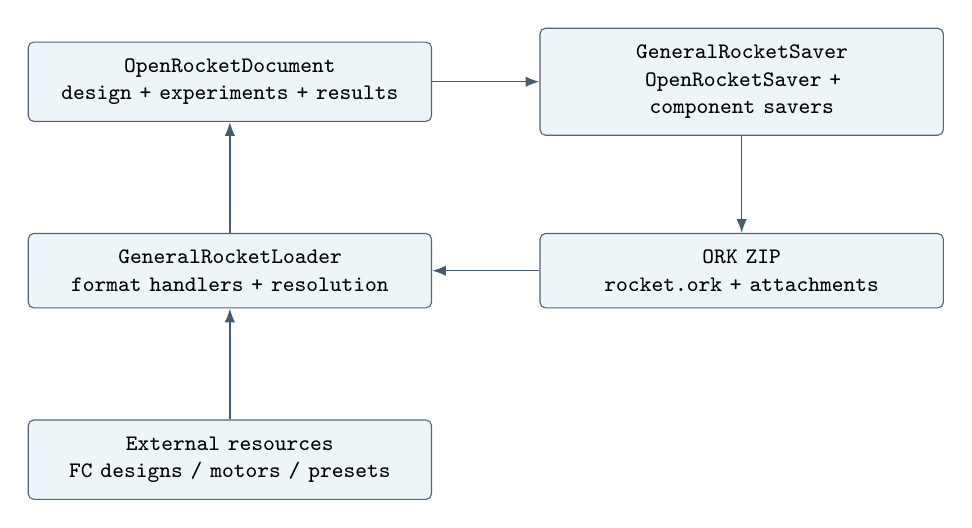
\begin{tikzpicture}
\simple{doc}{0,0}{OpenRocketDocument\\design + experiments + results}{4.7cm}
\simple{save}{6.5,0}{GeneralRocketSaver\\OpenRocketSaver + component savers}{4.7cm}
\simple{ork}{6.5,-2.4}{ORK ZIP\\rocket.ork + attachments}{4.7cm}
\simple{load}{0,-2.4}{GeneralRocketLoader\\format handlers + resolution}{4.7cm}
\simple{libs}{0,-4.8}{External resources\\FC designs / motors / presets}{4.7cm}
\draw[use] (doc)--(save); \draw[use] (save)--(ork);
\draw[use] (ork)--(load); \draw[use] (load)--(doc);
\draw[use] (libs)--(load);
\end{tikzpicture}}

For a new property, a successful UI edit and simulation run are only part of implementation. The saver must write it, the loader must restore it with an appropriate old-file default, copies must preserve it where intended, and freshness/provenance logic must recognize its effect. Round-trip coverage is especially useful for fields whose default value could hide an omitted serializer.

\sourceline{\source{core/src/main/java/info/openrocket/core/file/GeneralRocketSaver.java}{GeneralRocketSaver}; \source{core/src/main/java/info/openrocket/core/file/openrocket/OpenRocketSaver.java}{OpenRocketSaver}; \source{core/src/main/java/info/openrocket/core/document/StorageOptions.java}{StorageOptions}; \source{core/src/main/java/info/openrocket/core/simulation/motorbatch/MotorBatchIO.java}{MotorBatchIO}.}

\section{External FC designs and provenance}
An FC design is an external JSON library artifact, with board definitions, controller structure, source text, settings, and design metadata. Importing a design into the library creates a managed copy. The simulation's ORK state records the selected reference, component assignments, and provenance; it should not be mistaken for a self-contained reconstruction of every external design revision.

At run start, the selected design is resolved and frozen. Exact source/file hashes identify the content that was seen; semantic fingerprints distinguish behavior-changing edits from changes such as layout or naming that do not affect execution. A library file that later changes can make a result stale without changing the rocket geometry. Conversely, a result's recorded fingerprint is evidence of the run and should not be silently rewritten to match the current library.

Trust approval is local execution state, separate from the mere presence of a Java source string in an imported design. A shareable design cannot authorize arbitrary source execution simply by claiming it was approved on another machine. Chapter~\ref{ch:fc} gives the current schema, program compilation, and ownership details.

\section{Motor data, presets, materials, and appearances}
Motor loaders normalize supported thrust-curve formats into motor records. The installed motor configuration identifies which record, mount, ignition rule, and delay are in use. A database record is shared input data; propellant depletion and ignition time belong to a motor's runtime state. When resolving a saved design, motor identity and the available database both matter.

Component presets supply reusable catalog dimensions and material choices. Applying a preset populates component properties, but subsequent edits can make the object a custom design. Material density and surface properties feed the calculators; material names and user-defined material preferences help organize that data. Appearance textures and colors feed renderers and save attachments. A missing texture should not be confused with missing physical geometry.

\sourceline{\source{core/src/main/java/info/openrocket/core/file/motor/GeneralMotorLoader.java}{GeneralMotorLoader}; \source{core/src/main/java/info/openrocket/core/file/motor/RASPMotorLoader.java}{RASPMotorLoader}; \source{core/src/main/java/info/openrocket/core/file/motor/RockSimMotorLoader.java}{RockSimMotorLoader}.}

\section{How format handlers reconstruct objects}
Native and legacy XML handling is organized into small element handlers, attribute setters and component-specific adapters. \class{SimpleSAX} delegates parser events to the active \class{ElementHandler}; this abstraction assumes an element contains text or child elements rather than arbitrary mixed content. It pools a bounded number of readers and clears handlers before returning a reader. The structure lets nested motor, component, configuration and result elements be interpreted by the classes that understand their semantics.

The native savers mirror the component vocabulary with type-specific property output. Matching import handlers interpret stored units and enumerations, select defaults for absent fields, reconstruct configuration IDs and references, and accumulate warnings. XML tag names and persisted identifiers are part of the format contract. A class rename or a new enum value can therefore require explicit compatibility handling even when the Java compiler accepts the change.

Storage also includes document preferences, custom materials and appearances. Attachments are resolved through an attachment factory and can originate from a local file or a ZIP entry. Keeping image bytes in an ORK archive makes a design's decal portable; a filename string alone would depend on another machine's directory layout. External FC definitions have the separately documented library/provenance contract and must not be assumed to behave like embedded decal files.

\sourceline{\source{core/src/main/java/info/openrocket/core/file/simplesax/SimpleSAX.java}{SimpleSAX}; \source{core/src/main/java/info/openrocket/core/file/simplesax/ElementHandler.java}{ElementHandler}; \source{core/src/main/java/info/openrocket/core/file/openrocket/importt/DocumentPreferencesHandler.java}{document preferences import}.}

\section{RockSim and RASAero interoperability}
RockSim import and export use an explicit mapping between RockSim entities and OpenRocket components. The import handlers interpret dimensions, materials, placement and other supported attributes. The export path builds JAXB data-transfer objects from a copied rocket, including the format's named stage structure, unit conversions and component-specific fields. That copy permits conversion adjustments without rewriting the open design. The presence of both directions does not guarantee a lossless round trip for all OpenRocket features.

RASAero import/export has a separate mapping for design geometry, launch conditions, recovery and supported simulation data. Its exporter also uses JAXB DTOs and collects warnings/errors when the source design does not fit the target representation. A target format's component types, allowed stage structures and aerodynamic assumptions constrain what can be expressed. The conversion layer, rather than the core component superclass, owns these compatibility rules.

Use the native ORK format to retain OpenRocket-specific design and simulation semantics. RockSim and RASAero files are interoperability products whose warnings and converted values need to travel with the result. In particular, a foreign application's simulation settings are not automatically an executable equivalent of MIT FC tasks, ensembles or active control surfaces.

\sourceline{\source{core/src/main/java/info/openrocket/core/file/rocksim/export/RockSimSaver.java}{RockSimSaver}; \source{core/src/main/java/info/openrocket/core/file/rasaero/export/RASAeroSaver.java}{RASAeroSaver}.}

\section{OBJ mesh export and geometry-only products}
The Wavefront OBJ subsystem creates mesh geometry from supported components and active instance transforms. \class{OBJExporterFactory} dispatches to body-tube, transition/nose, fin, tube-fin, lug, ring, mass-object, rail-button and motor exporters. Assemblies provide placement and selection structure; they are skipped as independent solid meshes while their selected children can be exported. Low-level cylinder, disk, tube and polygon builders create vertices, faces, normals and texture coordinates.

Options control selected components and children, repeated instances, motors, level of detail, coordinate transformation, scale, origin offset, triangulation, appearance, and separate component files. Material export writes an accompanying MTL representation. Mesh utilities manage groups, material assignments, vertex bounds and triangulation. Changing tessellation resolution changes the exported polygonal approximation, not the parametric source design or aerodynamic strip discretization.

OBJ is useful for external rendering and geometry workflows. It contains a snapshot of surfaces, not the OpenRocket tree's editable relationships, flight configurations, motor event rules or simulator. The fin editor also exports SVG outlines through \class{SVGBuilder}. It constructs a continuous fin-and-tab path and emits a separate tab path when a tab extends beyond the fin, with chosen stroke color and width. This is a fabrication/vector-drawing export, not an arbitrary-SVG-to-rocket modeling pipeline.

\sourceline{\source{core/src/main/java/info/openrocket/core/file/wavefrontobj/export/OBJExporterFactory.java}{OBJExporterFactory}; \source{core/src/main/java/info/openrocket/core/file/wavefrontobj/export/OBJExportOptions.java}{OBJExportOptions}; \source{core/src/main/java/info/openrocket/core/file/wavefrontobj/DefaultObj.java}{mesh representation}; \source{core/src/main/java/info/openrocket/core/file/svg/export/SVGBuilder.java}{SVGBuilder}.}

\section{Motor and component catalog ingestion}
RASP \code{.eng} and RockSim \code{.rse} motor readers turn curve samples and metadata into \class{ThrustCurveMotor} records. General/ZIP loaders dispatch among supported input forms. The motor database groups and indexes records for lookup and selection; curve identity, manufacturer aliases and digest information help distinguish records that have similar labels. The \code{thrustcurve} package handles online request/response parsing and downloads, while the GUI presents search and selection. These are data acquisition and resolution paths, not an alternative thrust integrator.

Component presets use typed keys and property maps, XML transfer objects, material definitions and catalog loaders. The many CSV loaders in \code{preset.loader} normalize differing catalog columns and units into the same preset model. Presets cover supported component families such as tubes, transitions, noses, fins, rings, launch hardware and recovery parts. Material databases distinguish bulk, surface and line densities before a component calculates mass.

Bundled data can be serialized or preprocessed by developer utilities to reduce startup work. Runtime loaders also support user-supplied data. A successful catalog import only makes a part or curve available; a document still needs to select or instantiate it. Once a preset is applied, editing the component can clear its catalog association while preserving the resulting dimensions.

\sourceline{\source{core/src/main/java/info/openrocket/core/database/motor/ThrustCurveMotorSet.java}{grouped motor records}; \source{core/src/main/java/info/openrocket/core/preset/ComponentPreset.java}{typed preset}; \source{core/src/main/java/info/openrocket/core/database/ComponentPresetDatabaseLoader.java}{preset loading}.}


\section{Exporting to vanilla OpenRocket}
The current source adds a separate, deliberately lossy export targeting official OpenRocket 24.12. \class{VanillaOpenRocketExporter} writes a different file, prevents overwriting the source through equivalent paths or file identities, and first writes a complete temporary ZIP beside the destination. It streams the design without changing the open MIT document or copying all of its result histories.

\begin{tabularx}{\linewidth}{@{}L{4.2cm}Y@{}}\toprule
MIT feature & Vanilla representation or omission\\\midrule
Controlled trapezoidal fins & Ordinary fixed trapezoidal fins; control tabs removed\\
Triangular fin cross section & Rounded cross section; outline, thickness, and fillets retained\\
Large fin cant & Limited to the vanilla $\pm15^\circ$ range\\
Airbrake assembly & Ballast preserving mass and axial CG; deployment, drag, and detailed inertia lost\\
FC and other simulation extensions & Removed; ordinary saved recovery settings remain and need review\\
Results and telemetry & Omitted; simulations become unrun baselines\\
Ensembles, initial roll rate, motor-batch history & Ensemble/history data omitted and initial roll reset to zero\\
Custom expressions & Retained only if they and their transitive dependencies use supported channels\\\bottomrule
\end{tabularx}

The exporter reports the conversions. A vanilla rerun of this output is a different experiment, particularly when the MIT simulation used FC-only recovery or active aerodynamics. Matching mass and axial CG cannot preserve airbrake forces or detailed inertia. This path supports interoperability and baseline comparison, not equivalence of predicted flight behavior.

\sourceline{\source{core/src/main/java/info/openrocket/core/file/openrocket/VanillaOpenRocketExporter.java}{VanillaOpenRocketExporter}; \source{core/src/main/java/info/openrocket/core/file/openrocket/VanillaComponentSaver.java}{VanillaComponentSaver}.}

\chapter{Extension points and cross-cutting contracts}\label{ch:extensions}
\section{Plugins and dependency injection}
Application startup creates shared services through Guice modules. The plugin mechanism discovers types marked with \code{@Plugin}, identifies plugin interfaces, and binds matching implementations into injectable sets. Consumers request the relevant service set rather than hard-coding every implementation in the window that uses it. This supports families such as extension providers and optimization services.

Discovery and execution are different stages. Discovering an extension provider allows the UI to offer a capability. An individual simulation still owns its selected extension and configuration. A plugin JAR is application code with access to the process; it is not isolated merely because it was discovered dynamically.

\sourceline{\source{core/src/main/java/info/openrocket/core/plugin/Plugin.java}{Plugin}; \source{core/src/main/java/info/openrocket/core/plugin/PluginModule.java}{PluginModule}; \source{core/src/main/java/info/openrocket/core/plugin/AnnotationFinderImpl.java}{AnnotationFinderImpl}.}

\section{Simulation extensions versus listeners}
A \class{SimulationExtension} is the persistent, configurable feature attached to a simulation. It supplies identity and metadata, stores configuration, can declare result types, participates in document loading, and initializes runtime behavior. A \class{SimulationListener} is the callback object that actually observes or modifies an execution. One extension can create several collaborating runtime objects.

\class{AbstractSimulationExtension} copies its \class{Config} on cloning and on configuration access. This protects the configuration map from accidental sharing. It does not automatically deep-copy arbitrary subclass fields, open files, static variables, or external library state. An extension intended for repeated or parallel execution must explicitly define what is shared, what is immutable, and what is freshly created.

The FC extension follows this pattern: saved settings describe the computer, while initialization creates a listener that owns the per-flight runtime, sensor adapter, control bridges, and logs. The run's copied rocket prevents actuator outputs from rewriting the editor's design. Extension configuration, the FC library artifact, and transient firmware state are three different lifetimes.

\sourceline{\source{core/src/main/java/info/openrocket/core/simulation/extension/SimulationExtension.java}{SimulationExtension}; \source{core/src/main/java/info/openrocket/core/simulation/extension/AbstractSimulationExtension.java}{AbstractSimulationExtension}; \source{core/src/main/java/info/openrocket/core/simulation/extension/impl/ZephyrusFlightComputer.java}{ZephyrusFlightComputer}.}

\section{Callback families and numerical consequences}
\begin{tabularx}{\linewidth}{@{}L{4cm}YY@{}}\toprule
Interface & Typical role & Important boundary\\\midrule
\class{SimulationListener} & Run start/end and before/after-step behavior & A completed step differs from an internal derivative evaluation\\
\class{SimulationEventListener} & Event notifications and permitted event decisions & A listener may influence whether a queued event is accepted\\
\class{SimulationComputationListener} & Observe or replace atmospheric, mass, aerodynamic, thrust, or acceleration calculations & Calculations may occur several times within one RK step\\
\class{AbstractSimulationListener} & Default implementations across the callback families & Defaults and return sentinels are part of the API\\\bottomrule
\end{tabularx}

The listener helper invokes callbacks and interprets their return values. Depending on the callback, a boolean controls continuation or acceptance, a non-null object replaces a computed value, or a non-NaN scalar supplies an override. A new listener should follow the exact method contract rather than assuming all callbacks have the same convention.

Ordering matters when two listeners modify the same quantity. A random perturbation listener, an actuator listener, and a logging listener can otherwise observe different stages of the computation. Time-varying inputs should be functions of physical time and stable run identity where possible. Drawing a fresh random value every time the RK solver asks for acceleration makes the answer depend on the solver's internal evaluation count.

The FC's acquisition contract is more restrictive than a generic acceleration callback: it captures the appropriate first derivative state, associates it with the start of an accepted interval, and publishes coherent measurements after acceptance. Its virtual scheduler and deadline limiter then coordinate task completion with the engine. A generic \code{postStep} callback by itself does not reproduce that timing model.

\sourceline{\source{core/src/main/java/info/openrocket/core/simulation/listeners/SimulationListener.java}{SimulationListener}; \source{core/src/main/java/info/openrocket/core/simulation/listeners/SimulationEventListener.java}{SimulationEventListener}; \source{core/src/main/java/info/openrocket/core/simulation/listeners/SimulationComputationListener.java}{SimulationComputationListener}; \source{core/src/main/java/info/openrocket/core/simulation/listeners/SimulationListenerHelper.java}{SimulationListenerHelper}.}

\section{Scripts, Java boards, and legacy controllers}
The inherited scripting extension evaluates a configured script through an available script engine and exposes listener callbacks. On document load it disables enabled scripts that are not locally trusted. The language must be supported by the runtime and provide the required invocable interface. A script is therefore both a persistence concern and a runtime dependency.

MIT Java-board programs use the FC's own API, compilation, source-hash approval, measurement context, and task scheduler. They are not interchangeable with arbitrary OpenRocket simulation listeners. A board sees the FC context and submits commands through controlled bridges; a general simulation listener operates at the engine callback boundary. Both run in-process, but their intended APIs and scheduling contracts differ.

The source also retains older controller/listener paths, including \class{NewControlStepListener} and \class{AirbrakesControllerListener}. Their names and presence do not mean every FC run uses them as its controller implementation. Follow the actual registration and execution path from \class{Simulation} and the selected extensions. The current default RK6 selection and legacy timestep settings are especially easy to overlook when reading upstream classes alone.

\sourceline{\source{core/src/main/java/info/openrocket/core/simulation/extension/impl/ScriptingExtension.java}{ScriptingExtension}; \source{core/src/main/java/info/openrocket/core/simulation/listeners/NewControlStepListener.java}{NewControlStepListener}; \source{core/src/main/java/info/openrocket/core/simulation/listeners/AirbrakesControllerListener.java}{AirbrakesControllerListener}.}

\section{Units, numeric primitives, and coordinate utilities}
The utility layer supplies the shared mathematics used by geometry, physics, plots and export. \class{Coordinate} stores Cartesian values and an optional weight; that weight can represent mass in one calculation and normal-force weighting in another. \class{WorldCoordinate} represents geographic location. \class{Quaternion} and \class{Transformation} encode orientation and rigid transforms, while inertia and bounding-box helpers support physical aggregation and geometry. These types do not remove the need to know the frame and units expected by the caller.

Interpolation, polynomial fitting, numerical statistics, array operations, noise generation and mathematical tolerance helpers are centralized in \code{util}. A linear interpolator over a thrust curve, a polynomial interpolation across aerodynamic regimes, and a pink-noise wind process solve different problems even though all are numerical helpers. Their boundary behavior, extrapolation rules and random-state ownership are part of the calling subsystem's contract.

The units package also does more than multiply by a display scale. Temperature conversions can include an offset. Caliber units depend on a rocket reference diameter, and percentage-of-length units depend on a relevant length. Fractional inch formatting and axis tick generation are presentation concerns. \class{FixedUnitGroup} gives custom quantities a fixed unit representation; it does not supply automatic physical dimension checking for arbitrary expressions. Values and comparators keep unit-aware display/sorting separate from internal SI calculations.

\sourceline{\source{core/src/main/java/info/openrocket/core/util/Coordinate.java}{Coordinate}; \source{core/src/main/java/info/openrocket/core/util/Quaternion.java}{Quaternion}; \source{core/src/main/java/info/openrocket/core/util/Transformation.java}{Transformation}; \source{core/src/main/java/info/openrocket/core/unit/UnitGroup.java}{UnitGroup}; \source{core/src/main/java/info/openrocket/core/unit/CaliberUnit.java}{caliber conversion}.}

\section{Change tracking, traversal, formatting, and object lifetimes}
Modification IDs identify changes that invalidate cached geometry or results. Listener lists and change-source helpers distribute notifications; invalidation helpers make disposed UI bindings stop acting on old models. Mutability guards distinguish objects still being assembled from completed data that should be read. Safety checks can detect inappropriate access, but they do not make a mutable document or engine safe for arbitrary concurrent writes.

Rocket visitors provide reusable traversals, including component and motor-mount listing and breadth/depth traversal strategies. They let consumers such as reports or selectors visit the component tree without embedding every traversal in a dialog. Active physical instance traversal remains a separate question from visiting each design node once.

The formatting package creates readable rocket/configuration descriptions and substitutes motor/configuration information into names. It is separate from expression evaluation and unit conversion. Configuration naming can depend on selected motors, while a persistent configuration ID remains the stable reference. Localization wraps translators, contextual keys and resource bundles so these labels can change with language without redefining stored identities.

File, JAR, reflection, platform, build-property and configuration helpers support startup and persistence. Their small size should not obscure their effect: resource lookup and class loading can determine whether a packaged application behaves like a development launch. The jar-in-jar bootstrap classes and platform helpers belong to this deployment boundary.

\section{Warnings, application logs, and network services}
Simulation warnings/errors are structured model output with types and associated context. They can survive in results and appear in reports. Application logging is a different channel: Swing logging classes integrate log buffers, filtering, levels and diagnostic displays with the logging backend. A debug message about a repaint is not a flight warning; a flight warning should not disappear merely because a console logging threshold changes.

Communication services retrieve welcome/release information and update metadata, and support bug-report workflows. Connection abstractions separate network access from response interpretation. MIT-specific update selection and replacement are described in Chapter~\ref{ch:build}; inherited update classes also remain in the tree. The existence of a network helper does not mean every simulation uses the network. Normal physics calculations operate on the already resolved design, motor and environment inputs.

ThrustCurve communication has its own request/response and curve decoding classes. A motor download must become a validated local motor record before it can participate in a configuration. Network metadata, local catalog entries and a runtime motor's ignition clock have separate lifetimes and failure modes.

\sourceline{\source{core/src/main/java/info/openrocket/core/logging/WarningSet.java}{structured warnings}; \source{core/src/main/java/info/openrocket/core/communication/ConnectionSource.java}{connection abstraction}; \source{core/src/main/java/info/openrocket/core/communication/WelcomeInfoRetriever.java}{welcome information}; \source{core/src/main/java/info/openrocket/core/formatting/RocketDescriptorImpl.java}{rocket description formatting}.}

\section{Inherited extension examples and developer utilities}
The extension example packages illustrate air starts, CSV saving, damping-moment changes, simulation printing, roll control and stopping conditions. Providers expose examples to discovery; runtime listeners implement their behavior. These examples are useful API references, but merely finding a class in the tree does not establish that a particular simulation has enabled it. The same distinction applies to Swing extension configurators: a panel edits configuration, while the core extension installs execution behavior.

The scripting support includes script-engine discovery and a GraalJS factory in addition to the simulation extension itself. Language availability and the packaged runtime therefore affect script execution. The separately bundled expression parser is for arithmetic/array expressions and does not replace the script-engine API or the MIT Java-board runtime.

Developer utility packages contain localization generators/reports, motor-correlation tools, optimizer exercises, preset conversion/editing/serialization utilities, and small desktop support tools. They are not all normal startup services. Build scripts, resources, tests and documentation complete the codebase around the runtime Java packages; Appendix~\ref{app:packages} provides an explicit coverage inventory so these less visible areas are not omitted from the architecture map.


\section{A maintenance checklist by boundary}
When changing a component, check geometry and instance placement, mass and inertia, aerodynamic behavior, renderer geometry, copy/identity semantics, serialization, and editor units. When changing an engine path, check event ordering, accepted-step semantics, stage branches, recovery-stepper transitions, cancellation, and result timestamps. When changing an FC task, check input acquisition, completion visibility, state-transition behavior, actuator ownership, recovery deduplication, and logging.

When adding a simulation option or channel, check old-file defaults, freshness signatures, ensemble behavior, CSV and ORK persistence, imported-data behavior, and plots. A new channel may need circular, held-state, or event semantics rather than ordinary scalar averaging. When adding concurrency, inspect mutable static state and external outputs in addition to object clones.

These checks follow the application's ownership boundaries. They are more useful than assuming that a successful GUI demonstration proves persistence, parallel execution, or the timing of a numerical callback.

\section{Practical investigation routes}
For a surprising trajectory, inspect configuration and launch options, then events, warnings, active stages, mass, aerodynamic coefficients and the selected stepper. For FC behavior, compare physical truth, measurements, task completion, command publication and actuator latching separately.

For differing runs, compare source/artifact identity, rocket/FC fingerprints, seeds, environment, configuration and extensions. For a save/reload mismatch, trace the relevant saver and loader fields before investigating a repaint.

For a visual mismatch, identify whether the disputed value belongs to design geometry, a renderer or recorded playback data. A changed drawing does not automatically change aerodynamic forces or an already recorded flight.

\chapter{Builds, releases, verification, and documentation}\label{ch:build}
\section{Repository and build structure}
The parent repository contains the application checkout, documentation, firmware-related material, and platform packaging recipes. The convenient \code{clone/openrocket} path resolves to \code{clone/openrocket-release-24.12.RC.01} in this workspace. Run application Gradle commands from that source root. The root Gradle project assembles \code{core} and \code{swing}; its main entry point is \class{info.openrocket.swing.startup.OpenRocket}.

The build targets Java 17. \code{build.properties} distinguishes the upstream version from the MIT edition and version. The inspected source says upstream \code{24.12.RC.01} and MIT \code{6.4}. The executable artifact is a shadow JAR containing application classes and dependencies. The root thin JAR has a separate \code{plain} classifier so it cannot accidentally replace the executable launcher target.

\begin{lstlisting}[language=bash]
# From clone/openrocket, with JDK 17 selected:
./gradlew shadowJar

# Application verification, when changing application code:
./gradlew :core:test :swing:test

# MIT method documentation, API reference, and curated UML:
./gradlew verifyMitJavadoc rocketTeamJavadoc rocketTeamUml
\end{lstlisting}

These are build entry points, not a claim that the application tests were rerun while authoring this guide. Offline builds require the relevant dependencies and packaging downloads to be cached already. Platform graphics tests may require the appropriate native libraries and a display environment.

For edition 6.4, \code{shadowJar} produces \code{OpenRocket-MIT-v6.4.jar}. Finalizer tasks publish the compatibility alias \code{OpenRocket-24.12.RC.01.jar} atomically and generate the versioned JAR's \code{.sha256} companion. This keeps older desktop launchers working while allowing MIT-specific release naming. A filename alone is not proof of the commit that produced the bytes.

\sourceline{\source{settings.gradle}{settings.gradle}; \source{build.gradle}{build.gradle}; \source{core/src/main/resources/build.properties}{build.properties}; \source{gradle/mit-documentation.gradle}{mit-documentation.gradle}.}

\section{How the application is distributed}
The reviewed GitHub releases publish binary assets directly on the parent repository's release pages. The v6.4 release contains a universal macOS DMG and ZIP, a Windows x64 installer and checksum, the standalone/update JAR and checksum, and a combined checksum manifest. The full packages bundle Java; the standalone JAR requires a suitable local Java runtime.

The macOS recipe builds one application with a universal native launcher, one application JAR, and separate arm64 and x86\_64 Java runtimes. The launcher chooses the matching runtime instead of combining architecture-specific JVM files. The recipe produces an app bundle, DMG, and ZIP. The documented bundle uses ad-hoc signing rather than Developer ID signing and notarization.

Windows preparation builds the JAR and stages pinned runtime/tool inputs with checksums and provenance. Packaging runs on Windows through \code{jpackage} and WiX to produce a per-user x64 installer. The MIT installation has its own identity and includes the launcher compatibility needed by updates. The documented installer is unsigned. The packaging READMEs contain some version-specific historical examples; current version selection comes from the build properties and scripts.

The repository root does not contain a GitHub Actions publishing workflow for this process. An inherited workflow inside the nested OpenRocket source belongs to the upstream source layout and targets its own build/release assumptions. Its presence is not evidence that the parent repository automatically builds and publishes MIT installers. The concrete publication evidence is the release assets and the local packaging recipes.

\sourceline{\reposource{packaging/macos/package-macos.py}{package-macos.py}; \reposource{packaging/macos/launcher.c}{macOS launcher.c}; \reposource{packaging/windows/prepare-windows.py}{prepare-windows.py}; \reposource{packaging/windows/package-windows.ps1}{package-windows.ps1}; \href{https://github.com/MDNich/ActiveControl_MIT_RktTeam/releases/tag/v6.4}{published v6.4 release}.}

\section{Release evolution and the documented snapshot}
\begin{tabularx}{\linewidth}{@{}L{2.8cm}L{2.7cm}Y@{}}\toprule
Release & Published & Main milestone in the release notes\\\midrule
\code{v0.0.1} & 31 Aug 2025 & Controlled trapezoidal fins and native persistence\\
\code{functional_tab_ctrl} & 14 Sep 2025 & Functional customizable tab control\\
\code{v5} & 18 Nov 2025 & Airbrake component support; simulation work still announced as forthcoming\\
\code{v6} & 23 Jun 2026 & Triangular leading-edge support\\
\code{v6.1} & 4 Jul 2026 & MIT updates and reversible tab conversion preserving fin settings\\
\code{v6.2} & 21 Sep 2026 & Integrated FC simulation, 3D flight plots, Windows installer\\
\code{v6.3} & 26 Sep 2026 & Fin/tab previews, Windows update reliability, MIT release routing\\
\code{v6.4} & 13 Oct 2026 & Parallel motor comparisons, ensembles, and broader FC/control functionality\\\bottomrule
\end{tabularx}

The v6.4 tag resolves to \code{9f71a94196a6284ae2b574639aafbb2bf1bc175a}. This guide describes \code{7f0b67ee1c755ec89f154b0f0d2f4e23c843aa87}, three commits later. Subsequent changes include vanilla export, ensemble coefficient and wind-direction variation, parallel ensemble work, and fin-display corrections. Both snapshots carry the 6.4 edition label. Release-note claims describe the corresponding release and should not be projected backward onto every earlier package.

GitHub marks the reviewed v6.4 entry as a normal release, while the notes can still describe individual FC capabilities as beta. Repository release status and subsystem maturity are separate facts. For reproducible comparisons record the source commit, built JAR checksum, selected design/FC fingerprints, simulation options, seed, and runtime/platform context.

\sourceline{\href{https://github.com/MDNich/ActiveControl_MIT_RktTeam/releases}{MIT release history}; \href{https://github.com/MDNich/ActiveControl_MIT_RktTeam/compare/v6.4...7f0b67ee1c755ec89f154b0f0d2f4e23c843aa87}{source changes after v6.4}.}

\section{Automatic updates}
The MIT update retriever uses the MIT release feed and compares normalized numeric versions. It accepts an update only when the release version is greater than the running edition. It locates the versioned JAR and its digest, supplied by release metadata or a checksum asset. Consequently, a later commit with the same 6.4 label is not automatically distinguishable as an upgrade.

The installer downloads and verifies the JAR before replacement. Platform-specific handoff code waits for the running application to close, preserves a backup, replaces the target, and restarts the application. Windows has a dedicated helper for the packaged layout and writable per-user installations. Unsaved document handling belongs to the GUI path before installation proceeds.

This is a JAR update mechanism. It does not replace the bundled Java runtimes, native launcher, or installer metadata. Changes to those parts require a full package. A successful checksum check establishes integrity against the chosen release digest; it does not identify an unrecorded local source modification or make two same-version builds identical.

\sourceline{\source{core/src/main/java/info/openrocket/core/communication/MitUpdateInfoRetriever.java}{MitUpdateInfoRetriever}; \source{swing/src/main/java/info/openrocket/swing/gui/util/MitUpdateInstaller.java}{MitUpdateInstaller}; \source{swing/src/main/java/info/openrocket/swing/gui/util/WindowsUpdateHelper.java}{WindowsUpdateHelper}.}

\section{Verification layers}
Core tests can check component formulas, transforms, event timing, persistence round trips, ensemble determinism, controller state, and telemetry encoding without a full installer. FC replay and timing tests check scheduling and byte-level behavior against their fixtures. Swing tests check model adapters, configuration workflows, drawing helpers, and result interpretation. Packaged-runtime probes exercise the actual launcher, bundled JVM, native graphics libraries, and installer/update layout.

These layers answer different questions. A passing unit test does not demonstrate an Intel-native launch if the package was tested under Rosetta. A Windows x64 build tested under ARM64 emulation is useful evidence with a stated scope. Historical packaging reports and the incorporated FC chapter record their own test dates and counts. They are retained as historical evidence, not relabeled as verification of this documentation's later source snapshot.

This guide's creation checks the LaTeX build, cross-references, source-path references, unchanged reference copies, and rendered layout. It does not modify or requalify the application. Future code changes should choose tests according to the affected boundary, with special care for solver timing, GUI cancellation, persistence, and parallel execution.

\section{Maintaining this document}
\code{doc/main/main.tex} is the entry point. \code{preamble.tex} owns shared layout and diagram styles. Each numbered file in \code{sections/} owns one chapter. The FC chapter incorporates the full substantive body of the earlier report, adapting its scope and build notes and clarifying current engine/deadline behavior. The exact original TeX and PDF are retained in \code{reference/} for comparison.

From \code{doc/main}, run \code{./build.sh} to compile into \code{.build/} and copy the final PDF to \code{main.pdf}. The folder can also be opened as a LaTeX project with \code{main.tex} selected as its main file. The document uses standard TeX packages and vector TikZ diagrams; it has no external image-download or shell-escape requirement.

When changing the source edition, update the title page, commit-pinned link macros, release comparison, and any affected behavioral descriptions. Keep observations about current implementation separate from proposed designs in older reports. Update diagrams when ownership or order changes, and rebuild the table of contents, labels, and PDF bookmarks before reviewing the rendered pages.

\appendix
\titleformat{\chapter}[display]{\sffamily\bfseries\color{ink}\raggedright\hyphenpenalty=10000\exhyphenpenalty=10000}{\large APPENDIX \thechapter}{8pt}{\Huge}
\chapter{Source navigation and document provenance}\label{app:source}
\section{Where to begin by question}
Paths below are relative to \code{clone/openrocket}. Class names in the chapter source-entry lines link to the inspected commit. The table is a navigation index rather than an exhaustive inventory of every class.

\begin{longtable}{@{}L{3.4cm}L{7.0cm}L{5.4cm}@{}}
\toprule Question or subsystem & Start with & Then follow\\\midrule\endfirsthead
\toprule Question or subsystem & Start with & Then follow\\\midrule\endhead
Application startup & \code{swing/.../startup/OpenRocket.java}, \code{SwingStartup.java} & Application services, Guice modules, preferences, plugin discovery\\
Open design ownership & \code{core/.../document/OpenRocketDocument.java} & Rocket tree, simulations, expressions, undo, attachments\\
Component geometry & \code{core/.../rocketcomponent/RocketComponent.java} & Component subclasses, positioning, instances, change events\\
Motor/stage selection & \code{core/.../rocketcomponent/FlightConfiguration.java} & Configuration IDs, motor mounts, deployment and separation parameters\\
Mass and inertia & \code{core/.../masscalc/MassCalculator.java} & \code{MassCalculation}, \code{RigidBody}, component and motor mass\\
Aerodynamic coefficients & \code{core/.../aerodynamics/BarrowmanCalculator.java} & \code{barrowman/*Calc.java}, \code{FlightConditions}, \code{AerodynamicForces}\\
Motor curves and state & \code{core/.../motor/ThrustCurveMotor.java} & \code{MotorConfiguration}, \code{MotorClusterState}\\
Environment & \code{core/.../models/} & Atmosphere, gravity, wind; simulation geodetic computation\\
Saved experiment & \code{core/.../document/Simulation.java} & \code{SimulationOptions}, \code{SimulationConditions}, extension initialization\\
Event loop & \code{core/.../simulation/ModifiedEventSimulationEngine.java} & \code{BasicEventSimulationEngine}, event dispatch, branch changes\\
Ascent integration & \code{core/.../simulation/RK6SimulationStepper.java} & \code{RK4SimulationStepper}, \code{AbstractSimulationStepper}, listener helpers\\
Recovery descent & \code{core/.../simulation/BasicLandingStepper.java} & \code{AbstractEulerStepper}, \code{BasicTumbleStepper}, recovery events\\
FC host integration & \code{core/.../simulation/flightcomputer/} & Listener, sensor adapter, controllers, Java runtime, recovery and actuator bridges\\
Translated firmware & \code{core/src/main/java/edu/mit/rocket_team/} & Per-run RTFC, drivers, state machine, timing, telemetry; Chapter~\ref{ch:fc} class index\\
Repeated random trials & \code{core/.../simulation/ensemble/} & Runner, settings, perturbation listener, accumulator, archive\\
Motor comparisons & \code{core/.../simulation/motorbatch/} & Candidate/clearance rules, runner, metrics, reports, CSV and IO\\
Design optimization & \code{core/.../optimization/} & Rocket objective adapter, modifiers, constraints, search services\\
Desktop document UI & \code{swing/.../gui/main/} & \code{BasicFrame}, design/simulation/configuration panels\\
Component editing & \code{swing/.../gui/configdialog/} & Property adaptors, units, model setters, dialog disposal\\
Design figures & \code{swing/.../gui/rocketfigure/}, \code{figure3d/} & Shape helpers, renderers, selected-component overlays\\
Simulation dialogs & \code{swing/.../gui/simulation/}, \code{flightcomputer/} & Configuration, worker, motor-batch and FC editors\\
Plots and flight playback & \code{swing/.../gui/plot/} & Plot configuration, \code{TrajectoryData}, \code{Trajectory3DPanel}\\
Native persistence & \code{core/.../file/openrocket/} & Saver classes, \code{importt/} handlers, general loader/saver\\
Vanilla conversion & \code{VanillaOpenRocketExporter.java} in that package & \code{VanillaComponentSaver}, supported-expression filtering\\
Printing & \code{swing/.../gui/print/} & Print controller, printable components, visitor strategies\\
Updates & \code{core/.../communication/MitUpdateInfoRetriever.java} & Swing MIT update dialog, installer, Windows helper\\
Packaging & Parent-repository \code{packaging/macos/} and \code{packaging/windows/} & Runtime inputs, launchers, staging, checksums, verification reports\\
API documentation & \code{gradle/mit-documentation.gradle} & Source manifests, method audit tool, Javadoc and PlantUML tasks\\\bottomrule
\end{longtable}

In this table, \code{core/.../} abbreviates \code{core/src/main/java/info/openrocket/core/}; \code{swing/.../} abbreviates \code{swing/src/main/java/info/openrocket/swing/}. The firmware namespace is written in full because it does not use the OpenRocket package prefix.

\section{Reference hierarchy}
The primary authority for behavior in this guide is the inspected source commit. Current API comments, tests, and the FC architecture report supply contracts and examples. Release notes describe published artifacts at their tags. Older design proposals and implementation reports supply history, but some describe states that predate current recovery coupling, actuator coupling, namespaces, or parallel workflows.

The preserved FC inputs are:
\begin{itemize}
\item \code{reference/14-flight-computer-api-and-architecture.tex}: unchanged source copy of the original report.
\item \code{reference/14-flight-computer-api-and-architecture.pdf}: unchanged rendered copy supplied with that report.
\item \code{sections/08-flight-computer.tex}: integrated chapter, with current-source clarifications and shared document formatting.
\end{itemize}

The original report remains independently attributable to its source snapshot and verification statements. The integrated chapter's clarifications include the modified-engine/RK6 default, the actual FC step-limiting hook, and the distinction between controller-block epoch invalidation and Java-board task behavior. This guide does not treat instructions embedded in older reports as authorization to change or publish application code.

\chapter{Whole-codebase package atlas}\label{app:packages}

This appendix accounts for every Java source under the application's two \code{src/main/java} trees at the documented snapshot. It groups related packages by function and links them to the explanatory chapters. Counts are source files, not public classes, methods, lines of code, or a measure of subsystem importance. Nested types remain within their source file. The two module descriptors are counted separately from named packages.

The inventory contains \textbf{1,282 main Java files}: 826 in core and 456 in Swing, spanning 139 named packages plus the two module descriptors. The bundled expression parser and translated MIT firmware are included. \code{source-inventory.tsv}, beside the main document, lists every file, its package, subsystem, chapter label and source-relative path. It can be filtered to locate a package not printed in full below.

\code{tools/build_source_inventory.py} regenerates both this table and the per-file inventory from the local source tree. It requires every file to match an explicit documented subsystem and rejects uncovered paths. This is a coverage/navigation check, not a claim that every method has been individually explained or numerically validated. The prose describes subsystem behavior and the important interactions, with deeper treatment of geometry, forces and flight/control timing.


\section{Core module}

Package paths below are relative to \code{core/src/main/java/}. Except where written in full, the prefix is \code{info/openrocket/core/}. Each row includes its descendant packages unless a more specific row is listed.

\begin{longtable}{@{}L{4.6cm}L{0.8cm}L{10.2cm}@{}}\toprule Package family & Files & Function and guide location\\\midrule\endfirsthead

\toprule Package family & Files & Function and guide location\\\midrule\endhead

\code{module-info.java} & 1 & \textbf{Module declaration}. Exports and dependency requirements for the core module. Chapter~\ref{ch:runtime}.\\

\code{de/congrace/exp4j} & 22 & \textbf{Expression parser}. Bundled arithmetic parser, tokens, functions, variables and expression evaluation. Chapter~\ref{ch:results}.\\

\code{edu/mit/rocket_team} & 47 & \textbf{Translated flight computer}. AV/FC state, control and airbrake algorithms, instruments, per-run internals, telemetry, data and hardware abstractions. Chapter~\ref{ch:fc}.\\

\code{aerodynamics} & 14 & \textbf{Aerodynamics}. Calculator contracts, conditions and coefficients; Barrowman assembly and specialized body, fin, tube, rail-button and airbrake calculators. Chapter~\ref{ch:aero}.\\

\code{appearance} & 6 & \textbf{Appearance}. Colors, decals and default visual appearances, independent of physical surface finish. Chapter~\ref{ch:gui}.\\

\code{arch} & 1 & \textbf{Platform information}. Operating-system/platform identification for application behavior and resource selection. Chapter~\ref{ch:runtime}.\\

\code{communication} & 13 & \textbf{Application communication}. Connection abstraction, welcome/release retrieval, bug reports, upstream and MIT update metadata. Chapter~\ref{ch:build}.\\

\code{componentanalysis} & 6 & \textbf{Static analysis}. Analysis parameters, sweep domains, per-component coefficient data and static parameter sweeps. Chapter~\ref{ch:workflows}.\\

\code{database} & 11 & \textbf{Databases}. Async resource loading, catalog databases, motor lookup and grouped thrust-curve records. Chapter~\ref{ch:persistence}.\\

\code{document} & 12 & \textbf{Documents}. Design/simulation ownership, storage options, undo, document events and attachment references. Chapter~\ref{ch:runtime}.\\

\code{file/openrocket} & 87 & \textbf{Native ORK and vanilla export}. Document XML, component savers, import handlers, result/extension persistence and MIT-to-vanilla conversion. Chapter~\ref{ch:persistence}.\\

\code{file/rocksim} & 50 & \textbf{RockSim conversion}. Format constants and mappings, XML import handlers, export DTOs and saver. Chapter~\ref{ch:persistence}.\\

\code{file/rasaero} & 37 & \textbf{RASAero conversion}. Design, launch, recovery and simulation conversion through import handlers and export DTOs. Chapter~\ref{ch:persistence}.\\

\code{file/wavefrontobj} & 31 & \textbf{OBJ mesh export}. Mesh tuples/faces/groups/materials, triangulation, component exporters and cylinder/tube/disk/polygon builders. Chapter~\ref{ch:persistence}.\\

\code{file/svg} & 1 & \textbf{SVG utility}. Vector document/path construction used by fin-and-tab SVG export. Chapter~\ref{ch:persistence}.\\

\code{file/simplesax} & 6 & \textbf{XML parser delegation}. Element handlers, reader pooling and warning-aware SAX delegation. Chapter~\ref{ch:persistence}.\\

\code{file/motor} & 6 & \textbf{Motor-file loading}. RASP, RockSim and ZIP/general dispatch into thrust-curve records. Chapter~\ref{ch:persistence}.\\

\code{file/iterator} & 3 & \textbf{File iteration}. Directory/JAR resource iteration used by loaders. Chapter~\ref{ch:persistence}.\\

\code{file} & 17 & \textbf{General file services}. Format dispatch, load/save context, attachment handling, CSV export and shared file contracts. Chapter~\ref{ch:persistence}.\\

\code{formatting} & 4 & \textbf{Descriptions}. Rocket/configuration descriptions and motor-configuration name substitutions. Chapter~\ref{ch:extensions}.\\

\code{gui/util} & 1 & \textbf{Shared file filter}. File-filter adapter used by desktop and file-selection code. Chapter~\ref{ch:extensions}.\\

\code{l10n} & 7 & \textbf{Localization}. Translator interfaces, contextual/debug/resource translators and locale helpers. Chapter~\ref{ch:runtime}.\\

\code{logging} & 9 & \textbf{Structured diagnostics}. Warnings, errors, messages, priorities, abort information and message sets. Chapter~\ref{ch:extensions}.\\

\code{masscalc} & 4 & \textbf{Mass and inertia}. Component/motor aggregation, rigid-body properties and per-component mass-analysis entries. Chapter~\ref{ch:models}.\\

\code{material} & 3 & \textbf{Materials}. Bulk, sheet and line-density materials, groups and storage. Chapter~\ref{ch:models}.\\

\code{models/atmosphere} & 4 & \textbf{Atmosphere}. Atmospheric conditions, extended ISA and interpolation/model interfaces. Chapter~\ref{ch:models}.\\

\code{models/gravity} & 2 & \textbf{Gravity}. Gravity interface and WGS-based latitude/altitude model. Chapter~\ref{ch:models}.\\

\code{models/wind} & 4 & \textbf{Wind}. Wind interfaces, average/pink-noise and multilevel wind models. Chapter~\ref{ch:models}.\\

\code{motor} & 10 & \textbf{Propulsion}. Motor records, manufacturers/digests, installed configuration, ignition rules and runtime cluster state. Chapter~\ref{ch:models}.\\

\code{optimization/general} & 13 & \textbf{Numerical search}. Function/point contracts, caches/controllers, golden-section and multidirectional search. Chapter~\ref{ch:workflows}.\\

\code{optimization/rocketoptimization} & 24 & \textbf{Rocket optimization}. Physical objectives, goals, domains, modifiers and function adapter for trial designs. Chapter~\ref{ch:workflows}.\\

\code{optimization/services} & 5 & \textbf{Optimization discovery}. Services exposing available objectives and modifiable design/configuration variables. Chapter~\ref{ch:workflows}.\\

\code{plugin} & 6 & \textbf{Plugin discovery}. Annotations, class discovery and dependency-injection bindings. Chapter~\ref{ch:extensions}.\\

\code{preferences} & 3 & \textbf{Preferences}. Core-facing application/document preference models and defaults. Chapter~\ref{ch:runtime}.\\

\code{preset} & 53 & \textbf{Component catalogs}. Typed preset properties, material matching, CSV ingestion and XML DTOs/loaders. Chapter~\ref{ch:persistence}.\\

\code{rocketcomponent} & 76 & \textbf{Vehicle model}. All native parts and assemblies, placement strategies, instances, configuration parameters and change propagation. Chapter~\ref{ch:components}.\\

\code{rocketvisitors} & 4 & \textbf{Tree traversal}. Breadth/depth visitors and component/motor-mount listing. Chapter~\ref{ch:extensions}.\\

\code{scripting} & 3 & \textbf{Script engines}. Engine discovery and GraalJS integration for scripting support. Chapter~\ref{ch:extensions}.\\

\code{simulation/customexpression} & 5 & \textbf{Derived channels}. Expression definitions, ranges/functions and a result-writing listener. Chapter~\ref{ch:results}.\\

\code{simulation/ensemble} & 9 & \textbf{Ensembles}. Settings, random draws, isolated execution, perturbations, aggregate statistics and member archives. Chapter~\ref{ch:workflows}.\\

\code{simulation/exception} & 4 & \textbf{Run exceptions}. Calculation, listener/termination and other simulation exception contracts. Chapter~\ref{ch:engine}.\\

\code{simulation/extension} & 27 & \textbf{Simulation features}. Persistent extension/provider contracts, implementations and inherited examples. Chapter~\ref{ch:extensions}.\\

\code{simulation/flightcomputer} & 19 & \textbf{FC host integration}. Runtime listener, sensors, scheduler/control bridges, Java programs, design library, recovery and logs. Chapter~\ref{ch:fc}.\\

\code{simulation/listeners} & 20 & \textbf{Simulation callbacks}. Computation/event/step interfaces, dispatch helpers, controllers, examples and system stopping/coast listeners. Chapter~\ref{ch:extensions}.\\

\code{simulation/motorbatch} & 10 & \textbf{Motor comparisons}. Candidate selection, fit/clearance, isolated cases, metrics, report history, CSV and persistence. Chapter~\ref{ch:workflows}.\\

\code{simulation} & 27 & \textbf{Flight execution and data}. Options/conditions/status, event engines, RK/Euler/mode steppers, events and typed flight histories. Chapter~\ref{ch:engine}.\\

\code{startup} & 2 & \textbf{Core application services}. Shared application service access and exception handling. Chapter~\ref{ch:runtime}.\\

\code{thrustcurve} & 12 & \textbf{Online motor data}. API request/response objects, XML parsing, curve decoding/downloads and serialization helpers. Chapter~\ref{ch:persistence}.\\

\code{unit} & 16 & \textbf{Units}. Conversion, unit groups, values, comparison, fractional formatting and axis ticks. Chapter~\ref{ch:extensions}.\\

\code{util} & 64 & \textbf{Shared utilities}. Coordinates/transforms, numerics, interpolation, noise, statistics, identity, listeners, mutability and resource helpers. Chapter~\ref{ch:extensions}.\\

\code{utils} & 5 & \textbf{Developer utilities}. Localization generation/reporting, motor comparison and optimizer exercise programs. Chapter~\ref{ch:extensions}.\\

\bottomrule\end{longtable}

\section{Swing module}

Package paths below are relative to \code{swing/src/main/java/}. Except where written in full, the prefix is \code{info/openrocket/swing/}. Each row includes its descendant packages unless a more specific row is listed.

\begin{longtable}{@{}L{4.6cm}L{0.8cm}L{10.2cm}@{}}\toprule Package family & Files & Function and guide location\\\midrule\endfirsthead

\toprule Package family & Files & Function and guide location\\\midrule\endhead

\code{module-info.java} & 1 & \textbf{Module declaration}. Exports and dependencies for the desktop module. Chapter~\ref{ch:runtime}.\\

\code{communication} & 1 & \textbf{Desktop communication}. Maps release assets to operating platforms and selects installer download links. Chapter~\ref{ch:build}.\\

\code{file} & 5 & \textbf{Desktop file adapters}. Simulation-table CSV, motor-loading helper, Photo Studio settings adapters and OBJ option chooser. Chapter~\ref{ch:persistence}.\\

\code{gui/adaptors} & 17 & \textbf{Property bindings}. Boolean/numeric/enum and related Swing models connected to core properties and units. Chapter~\ref{ch:gui}.\\

\code{gui/components} & 29 & \textbf{Shared controls}. Reusable buttons, fields, selectors, tables and compass controls. Chapter~\ref{ch:gui}.\\

\code{gui/configdialog} & 37 & \textbf{Component editors}. Specialized part dialogs plus appearance, placement, instances, material and override controls. Chapter~\ref{ch:gui}.\\

\code{gui/customexpression} & 7 & \textbf{Expression editor}. Expression names, symbols, units, functions, editing and validation UI. Chapter~\ref{ch:results}.\\

\code{gui/dialogs/componentanalysis} & 10 & \textbf{Analysis UI}. Component coefficients, selections, sweep configuration, plotting and export. Chapter~\ref{ch:workflows}.\\

\code{gui/dialogs/flightconfiguration} & 6 & \textbf{Configuration dialogs}. Motor-mount, ignition, separation, deployment and naming controls. Chapter~\ref{ch:gui}.\\

\code{gui/dialogs/motor} & 15 & \textbf{Motor selection}. Motor information/filtering and thrust-curve selection, comparison, plotting and download UI. Chapter~\ref{ch:gui}.\\

\code{gui/dialogs/optimization} & 6 & \textbf{Optimization UI}. Variable/goal selection, background search, progress and plotted history. Chapter~\ref{ch:workflows}.\\

\code{gui/dialogs/preferences} & 12 & \textbf{Preferences UI}. Application defaults, units, materials, launch, simulation, display and graphics choices. Chapter~\ref{ch:runtime}.\\

\code{gui/dialogs/preset} & 5 & \textbf{Preset dialogs}. Catalog selection, editing and associated model/dialog helpers. Chapter~\ref{ch:persistence}.\\

\code{gui/dialogs} & 18 & \textbf{Application dialogs}. Shared desktop dialogs including scaling, print setup, warnings and application interactions. Chapter~\ref{ch:gui}.\\

\code{gui/figure3d/photo} & 16 & \textbf{Photo Studio}. Posed rocket scene, camera/light settings, exhaust rendering and sky/background implementations. Chapter~\ref{ch:gui}.\\

\code{gui/figure3d} & 12 & \textbf{3D design renderer}. JOGL view/render orchestration and component geometry/material rendering. Chapter~\ref{ch:gui}.\\

\code{gui/figureelements} & 5 & \textbf{Figure overlays}. Additional figure annotations and derived-property markers. Chapter~\ref{ch:gui}.\\

\code{gui/flightcomputer} & 6 & \textbf{FC design editor}. Board/program/controller design, assignments, settings and diagnostics. Chapter~\ref{ch:fc}.\\

\code{gui/help/tours} & 9 & \textbf{Guided help}. Tour data loading, panels and guided-help presentation. Chapter~\ref{ch:gui}.\\

\code{gui/main} & 35 & \textbf{Document windows}. Main panels/actions, component tree, selection/drag operations and flight-configuration tables. Chapter~\ref{ch:gui}.\\

\code{gui/plot} & 18 & \textbf{Results and playback}. Plot definitions/axes/events, simulation charts, trajectory adaptation and 3D playback. Chapter~\ref{ch:results}.\\

\code{gui/preset} & 6 & \textbf{Preset widgets}. Catalog tables, sorting/filtering and preset result interactions. Chapter~\ref{ch:persistence}.\\

\code{gui/print} & 36 & \textbf{Printing}. Reports/templates, paper/layout controls, selection tree and component visitor strategies. Chapter~\ref{ch:results}.\\

\code{gui/rocketfigure} & 24 & \textbf{2D component shapes}. Side/back-view shape providers for supported components and fin-profile drawing. Chapter~\ref{ch:gui}.\\

\code{gui/scalefigure} & 7 & \textbf{Scaled design view}. Zoomable figures, coordinate mapping, rulers and rocket-view integration. Chapter~\ref{ch:gui}.\\

\code{gui/simulation} & 17 & \textbf{Simulation UI}. Run/configuration dialogs, workers, launch/wind settings and motor-batch workflows. Chapter~\ref{ch:workflows}.\\

\code{gui/theme} & 2 & \textbf{Themes}. Application theme definitions and selection behavior. Chapter~\ref{ch:gui}.\\

\code{gui/util} & 29 & \textbf{Desktop utilities}. Icons, platform/window/model helpers, validation, update installation and related shared operations. Chapter~\ref{ch:gui}.\\

\code{gui/watcher} & 6 & \textbf{External-file watching}. Watch services, events and reactions for desktop files/assets. Chapter~\ref{ch:gui}.\\

\code{gui/widgets} & 11 & \textbf{Additional widgets}. Reusable text/table/selection and presentation widgets. Chapter~\ref{ch:gui}.\\

\code{gui} & 3 & \textbf{GUI service boundary}. Top-level desktop service/GUI support classes. Chapter~\ref{ch:gui}.\\

\code{logging} & 13 & \textbf{Desktop logs}. Logging backend integration, buffers, filters and diagnostic display support. Chapter~\ref{ch:extensions}.\\

\code{simulation/extension} & 7 & \textbf{Extension configuration UI}. Configurator contracts, examples and editors for core simulation extensions. Chapter~\ref{ch:extensions}.\\

\code{startup} & 15 & \textbf{Desktop bootstrap}. Entry/startup classes, jar-in-jar loading and injected service providers. Chapter~\ref{ch:runtime}.\\

\code{utils} & 10 & \textbf{Desktop/developer utilities}. Standalone application setup, preset tools/converters, scripting and small formatting/input helpers. Chapter~\ref{ch:extensions}.\\

\bottomrule\end{longtable}

\section{Resources, tests, and non-runtime source}
The main resource trees contain 107 core files and 301 Swing files in this snapshot. Core resources include build metadata, translations and data catalogs, serialized thrust curves, catalog CSV inputs, and example ORK designs. Swing resources include service registrations, icons, fonts, themes, textures, sky/exhaust assets, a graphics shader, help content and the Windows update helper. These files can affect runtime behavior or presentation despite not appearing in the Java count.

The test trees contain 169 core Java files and 34 Swing Java files, with 30 and 3 test-resource files respectively. They contain test cases and shared fixtures/helpers, not 203 independently counted test methods. The tests cover selected contracts across models, files, simulations and UI support; the mere existence of a test tree does not establish coverage of every formula or platform. Historical test results are identified separately in the FC and build chapters.

The source-root build files, Gradle wrapper/configuration, module builds and documentation tasks select dependencies, compilation, testing and packaging. \code{tools/documentation} contains source-inventory/documentation tooling. \code{fileformat.txt}, \code{docs/}, \code{doc/}, example/test-writing designs, developer instructions and release material explain interfaces and workflows outside executable classes. The inherited \code{install4j/}, \code{snap/} and workflow files reflect upstream distribution arrangements; the parent repository's \code{packaging/} recipes implement the MIT packages described in Chapter~\ref{ch:build}.

The parent repository also contains firmware-related work and development documentation outside the OpenRocket application checkout. Those are context and integration inputs; this guide's exhaustive Java inventory is specifically the OpenRocket core/Swing codebase plus the firmware translation embedded within core. Generated binaries, IDE metadata and crash logs are not additional application subsystems.

\end{document}
